\documentclass[twoside]{book}

% Packages required by doxygen
\usepackage{fixltx2e}
\usepackage{calc}
\usepackage{doxygen}
\usepackage[export]{adjustbox} % also loads graphicx
\usepackage{graphicx}
\usepackage[utf8]{inputenc}
\usepackage{makeidx}
\usepackage{multicol}
\usepackage{multirow}
\PassOptionsToPackage{warn}{textcomp}
\usepackage{textcomp}
\usepackage[nointegrals]{wasysym}
\usepackage[table]{xcolor}

% Font selection
\usepackage[T1]{fontenc}
\usepackage[scaled=.90]{helvet}
\usepackage{courier}
\usepackage{amssymb}
\usepackage{sectsty}
\renewcommand{\familydefault}{\sfdefault}
\allsectionsfont{%
  \fontseries{bc}\selectfont%
  \color{darkgray}%
}
\renewcommand{\DoxyLabelFont}{%
  \fontseries{bc}\selectfont%
  \color{darkgray}%
}
\newcommand{\+}{\discretionary{\mbox{\scriptsize$\hookleftarrow$}}{}{}}

% Page & text layout
\usepackage{geometry}
\geometry{%
  a4paper,%
  top=2.5cm,%
  bottom=2.5cm,%
  left=2.5cm,%
  right=2.5cm%
}
\tolerance=750
\hfuzz=15pt
\hbadness=750
\setlength{\emergencystretch}{15pt}
\setlength{\parindent}{0cm}
\setlength{\parskip}{3ex plus 2ex minus 2ex}
\makeatletter
\renewcommand{\paragraph}{%
  \@startsection{paragraph}{4}{0ex}{-1.0ex}{1.0ex}{%
    \normalfont\normalsize\bfseries\SS@parafont%
  }%
}
\renewcommand{\subparagraph}{%
  \@startsection{subparagraph}{5}{0ex}{-1.0ex}{1.0ex}{%
    \normalfont\normalsize\bfseries\SS@subparafont%
  }%
}
\makeatother

% Headers & footers
\usepackage{fancyhdr}
\pagestyle{fancyplain}
\fancyhead[LE]{\fancyplain{}{\bfseries\thepage}}
\fancyhead[CE]{\fancyplain{}{}}
\fancyhead[RE]{\fancyplain{}{\bfseries\leftmark}}
\fancyhead[LO]{\fancyplain{}{\bfseries\rightmark}}
\fancyhead[CO]{\fancyplain{}{}}
\fancyhead[RO]{\fancyplain{}{\bfseries\thepage}}
\fancyfoot[LE]{\fancyplain{}{}}
\fancyfoot[CE]{\fancyplain{}{}}
\fancyfoot[RE]{\fancyplain{}{\bfseries\scriptsize Generated by Doxygen }}
\fancyfoot[LO]{\fancyplain{}{\bfseries\scriptsize Generated by Doxygen }}
\fancyfoot[CO]{\fancyplain{}{}}
\fancyfoot[RO]{\fancyplain{}{}}
\renewcommand{\footrulewidth}{0.4pt}
\renewcommand{\chaptermark}[1]{%
  \markboth{#1}{}%
}
\renewcommand{\sectionmark}[1]{%
  \markright{\thesection\ #1}%
}

% Indices & bibliography
\usepackage{natbib}
\usepackage[titles]{tocloft}
\setcounter{tocdepth}{3}
\setcounter{secnumdepth}{5}
\makeindex

% Hyperlinks (required, but should be loaded last)
\usepackage{ifpdf}
\ifpdf
  \usepackage[pdftex,pagebackref=true]{hyperref}
\else
  \usepackage[ps2pdf,pagebackref=true]{hyperref}
\fi
\hypersetup{%
  colorlinks=true,%
  linkcolor=blue,%
  citecolor=blue,%
  unicode%
}

% Custom commands
\newcommand{\clearemptydoublepage}{%
  \newpage{\pagestyle{empty}\cleardoublepage}%
}

\usepackage{caption}
\captionsetup{labelsep=space,justification=centering,font={bf},singlelinecheck=off,skip=4pt,position=top}

%===== C O N T E N T S =====

\begin{document}

% Titlepage & ToC
\hypersetup{pageanchor=false,
             bookmarksnumbered=true,
             pdfencoding=unicode
            }
\pagenumbering{alph}
\begin{titlepage}
\vspace*{7cm}
\begin{center}%
{\Large Automatic Curtain \\[1ex]\large M\+VP }\\
\vspace*{1cm}
{\large Generated by Doxygen 1.8.13}\\
\end{center}
\end{titlepage}
\clearemptydoublepage
\pagenumbering{roman}
\tableofcontents
\clearemptydoublepage
\pagenumbering{arabic}
\hypersetup{pageanchor=true}

%--- Begin generated contents ---
\chapter{Namespace Index}
\section{Namespace List}
Here is a list of all namespaces with brief descriptions\+:\begin{DoxyCompactList}
\item\contentsline{section}{\hyperlink{namespaceCONFIG__SET}{C\+O\+N\+F\+I\+G\+\_\+\+S\+ET} \\*Namespace to be used for constants/enums }{\pageref{namespaceCONFIG__SET}}{}
\end{DoxyCompactList}

\chapter{Class Index}
\section{Class List}
Here are the classes, structs, unions and interfaces with brief descriptions\+:\begin{DoxyCompactList}
\item\contentsline{section}{\hyperlink{classAlexaInteraction}{Alexa\+Interaction} }{\pageref{classAlexaInteraction}}{}
\item\contentsline{section}{\hyperlink{classConnectivity}{Connectivity} }{\pageref{classConnectivity}}{}
\item\contentsline{section}{\hyperlink{classController}{Controller} }{\pageref{classController}}{}
\item\contentsline{section}{\hyperlink{classIndicator}{Indicator} }{\pageref{classIndicator}}{}
\item\contentsline{section}{\hyperlink{classLogging}{Logging} }{\pageref{classLogging}}{}
\item\contentsline{section}{\hyperlink{classManualInteraction}{Manual\+Interaction} }{\pageref{classManualInteraction}}{}
\item\contentsline{section}{\hyperlink{classMotorDriver}{Motor\+Driver} }{\pageref{classMotorDriver}}{}
\item\contentsline{section}{\hyperlink{classStorage}{Storage} }{\pageref{classStorage}}{}
\end{DoxyCompactList}

\chapter{File Index}
\section{File List}
Here is a list of all files with brief descriptions\+:\begin{DoxyCompactList}
\item\contentsline{section}{mvp/\hyperlink{mvp_8ino}{mvp.\+ino} }{\pageref{mvp_8ino}}{}
\item\contentsline{section}{mvp/src/alexa\+\_\+interaction/\hyperlink{alexa__interaction_8cpp}{alexa\+\_\+interaction.\+cpp} \\*Contains algorithms for handling alexa requests and make appropriate call at every request }{\pageref{alexa__interaction_8cpp}}{}
\item\contentsline{section}{mvp/src/alexa\+\_\+interaction/\hyperlink{alexa__interaction_8h}{alexa\+\_\+interaction.\+h} \\*Defines structure for class which will be interacting with alexa A\+PI }{\pageref{alexa__interaction_8h}}{}
\item\contentsline{section}{mvp/src/config/\hyperlink{config_8h}{config.\+h} \\*This header file contains all the constants and enum that will be used throughout the repository like specific pins, mapping from state to led color etc }{\pageref{config_8h}}{}
\item\contentsline{section}{mvp/src/connectivity/\hyperlink{connectivity_8cpp}{connectivity.\+cpp} \\*Contains algorithms related to connecting to Wi\+Fi, O\+TA updates and webpage display }{\pageref{connectivity_8cpp}}{}
\item\contentsline{section}{mvp/src/connectivity/\hyperlink{connectivity_8h}{connectivity.\+h} \\*Define overall structure for class containing Wi\+Fi, O\+TA and webpage functionality }{\pageref{connectivity_8h}}{}
\item\contentsline{section}{mvp/src/connectivity/\hyperlink{webpage_8h}{webpage.\+h} \\*Contains resources related to webpage for eg. html code }{\pageref{webpage_8h}}{}
\item\contentsline{section}{mvp/src/controller/\hyperlink{controller_8cpp}{controller.\+cpp} \\*Contains algorithms which controls the whole device from initialization to giving commands to every subsystem }{\pageref{controller_8cpp}}{}
\item\contentsline{section}{mvp/src/controller/\hyperlink{controller_8h}{controller.\+h} \\*Defines the structure of the main controller of the device }{\pageref{controller_8h}}{}
\item\contentsline{section}{mvp/src/indicator/\hyperlink{indicator_8cpp}{indicator.\+cpp} \\*Contains algorithms for R\+GB L\+ED }{\pageref{indicator_8cpp}}{}
\item\contentsline{section}{mvp/src/indicator/\hyperlink{indicator_8h}{indicator.\+h} \\*Contains structure for R\+GB L\+ED (C\+OM 11821), uses F\+A\+S\+T\+Led library for controlling the L\+ED }{\pageref{indicator_8h}}{}
\item\contentsline{section}{mvp/src/logging/\hyperlink{logging_8cpp}{logging.\+cpp} \\*Contains all algorithms for maintaing device logs }{\pageref{logging_8cpp}}{}
\item\contentsline{section}{mvp/src/logging/\hyperlink{logging_8h}{logging.\+h} \\*Defines code structure for logging of device }{\pageref{logging_8h}}{}
\item\contentsline{section}{mvp/src/manual\+\_\+interaction/\hyperlink{manual__interaction_8cpp}{manual\+\_\+interaction.\+cpp} \\*Contains algorithms to detect a users manual interaction with the device, specifically push buttons }{\pageref{manual__interaction_8cpp}}{}
\item\contentsline{section}{mvp/src/manual\+\_\+interaction/\hyperlink{manual__interaction_8h}{manual\+\_\+interaction.\+h} \\*Defines structure for manual interaction with device }{\pageref{manual__interaction_8h}}{}
\item\contentsline{section}{mvp/src/motor\+\_\+driver/\hyperlink{motor__driver_8cpp}{motor\+\_\+driver.\+cpp} \\*Contains algorithms for controlling stepper motor }{\pageref{motor__driver_8cpp}}{}
\item\contentsline{section}{mvp/src/motor\+\_\+driver/\hyperlink{motor__driver_8h}{motor\+\_\+driver.\+h} \\*Defines structure for controller of stepper motor, uses library T\+M\+C2209 for this usecase }{\pageref{motor__driver_8h}}{}
\item\contentsline{section}{mvp/src/storage/\hyperlink{storage_8cpp}{storage.\+cpp} \\*Contains algorithms to read and write appropriate device data to Flash }{\pageref{storage_8cpp}}{}
\item\contentsline{section}{mvp/src/storage/\hyperlink{storage_8h}{storage.\+h} \\*Defines structure for Flash storage for E\+S\+P32 }{\pageref{storage_8h}}{}
\end{DoxyCompactList}

\chapter{Namespace Documentation}
\hypertarget{namespaceCONFIG__SET}{}\section{C\+O\+N\+F\+I\+G\+\_\+\+S\+ET Namespace Reference}
\label{namespaceCONFIG__SET}\index{C\+O\+N\+F\+I\+G\+\_\+\+S\+ET@{C\+O\+N\+F\+I\+G\+\_\+\+S\+ET}}


Namespace to be used for constants/enums.  


\subsection*{Classes}
\begin{DoxyCompactItemize}
\item 
struct \hyperlink{structCONFIG__SET_1_1CALIB__PARAMS}{C\+A\+L\+I\+B\+\_\+\+P\+A\+R\+A\+MS}
\item 
struct \hyperlink{structCONFIG__SET_1_1DEVICE__CRED}{D\+E\+V\+I\+C\+E\+\_\+\+C\+R\+ED}
\item 
struct \hyperlink{structCONFIG__SET_1_1MOTION__REQUEST}{M\+O\+T\+I\+O\+N\+\_\+\+R\+E\+Q\+U\+E\+ST}
\end{DoxyCompactItemize}
\subsection*{Typedefs}
\begin{DoxyCompactItemize}
\item 
using \hyperlink{namespaceCONFIG__SET_a8816a22e7885d027a52bfa0d24fa9008}{time\+\_\+var} = std\+::chrono\+::time\+\_\+point$<$ std\+::chrono\+::system\+\_\+clock $>$
\item 
using \hyperlink{namespaceCONFIG__SET_a7a1c6f926aead4885c03f1fbeee693ce}{current\+\_\+time} = std\+::chrono\+::system\+\_\+clock
\end{DoxyCompactItemize}
\subsection*{Enumerations}
\begin{DoxyCompactItemize}
\item 
enum \hyperlink{namespaceCONFIG__SET_ac5c2592b79bead7e6497c37cddc401e6}{O\+P\+E\+R\+A\+T\+I\+O\+N\+\_\+\+M\+O\+DE} \{ \hyperlink{namespaceCONFIG__SET_ac5c2592b79bead7e6497c37cddc401e6ab5859d8721cfdc0312b2838b9c985bc1}{O\+P\+E\+R\+A\+T\+I\+O\+N\+\_\+\+M\+O\+D\+E\+::\+R\+E\+S\+ET}, 
\hyperlink{namespaceCONFIG__SET_ac5c2592b79bead7e6497c37cddc401e6aa49182544bf417d2e02cae1f35c9c8b8}{O\+P\+E\+R\+A\+T\+I\+O\+N\+\_\+\+M\+O\+D\+E\+::\+M\+A\+I\+N\+T\+E\+N\+A\+N\+CE}, 
\hyperlink{namespaceCONFIG__SET_ac5c2592b79bead7e6497c37cddc401e6a2e40ad879e955201df4dedbf8d479a12}{O\+P\+E\+R\+A\+T\+I\+O\+N\+\_\+\+M\+O\+D\+E\+::\+U\+S\+ER}, 
\hyperlink{namespaceCONFIG__SET_ac5c2592b79bead7e6497c37cddc401e6ad4cd0dabcf4caa22ad92fab40844c786}{O\+P\+E\+R\+A\+T\+I\+O\+N\+\_\+\+M\+O\+D\+E\+::\+NA}
 \}
\item 
enum \hyperlink{namespaceCONFIG__SET_aaf9764960ee214f0eaabd2461e30e932}{L\+O\+G\+\_\+\+T\+Y\+PE} \{ \hyperlink{namespaceCONFIG__SET_aaf9764960ee214f0eaabd2461e30e932a551b723eafd6a31d444fcb2f5920fbd3}{L\+O\+G\+\_\+\+T\+Y\+P\+E\+::\+I\+N\+FO}, 
\hyperlink{namespaceCONFIG__SET_aaf9764960ee214f0eaabd2461e30e932abb1ca97ec761fc37101737ba0aa2e7c5}{L\+O\+G\+\_\+\+T\+Y\+P\+E\+::\+E\+R\+R\+OR}, 
\hyperlink{namespaceCONFIG__SET_aaf9764960ee214f0eaabd2461e30e932a32bd8a1db2275458673903bdb84cb277}{L\+O\+G\+\_\+\+T\+Y\+P\+E\+::\+W\+A\+RN}
 \}
\item 
enum \hyperlink{namespaceCONFIG__SET_a3c4daebec2ea4e9f6affb5b3abbeb863}{L\+O\+G\+\_\+\+C\+L\+A\+SS} \{ \newline
\hyperlink{namespaceCONFIG__SET_a3c4daebec2ea4e9f6affb5b3abbeb863a42e074e8564dad9034ef033c6a6cf8b6}{L\+O\+G\+\_\+\+C\+L\+A\+S\+S\+::\+C\+O\+N\+T\+R\+O\+L\+L\+ER}, 
\hyperlink{namespaceCONFIG__SET_a3c4daebec2ea4e9f6affb5b3abbeb863afe45874d234b693c3648a37d604b0865}{L\+O\+G\+\_\+\+C\+L\+A\+S\+S\+::\+C\+O\+N\+N\+E\+C\+T\+I\+V\+I\+TY}, 
\hyperlink{namespaceCONFIG__SET_a3c4daebec2ea4e9f6affb5b3abbeb863a2b254b1e77ef0d4fe30639ee576bf05d}{L\+O\+G\+\_\+\+C\+L\+A\+S\+S\+::\+I\+N\+D\+I\+C\+A\+T\+OR}, 
\hyperlink{namespaceCONFIG__SET_a3c4daebec2ea4e9f6affb5b3abbeb863a042bca9f4ffd4cb8530fa2a9035e00c3}{L\+O\+G\+\_\+\+C\+L\+A\+S\+S\+::\+L\+O\+G\+G\+I\+NG}, 
\newline
\hyperlink{namespaceCONFIG__SET_a3c4daebec2ea4e9f6affb5b3abbeb863a0b83d32b63ae6ca0805d471c407c39a8}{L\+O\+G\+\_\+\+C\+L\+A\+S\+S\+::\+M\+A\+N\+U\+A\+L\+\_\+\+I\+N\+T\+E\+R\+A\+C\+T\+I\+ON}, 
\hyperlink{namespaceCONFIG__SET_a3c4daebec2ea4e9f6affb5b3abbeb863aef2f278882c5090b495fea73f0f14150}{L\+O\+G\+\_\+\+C\+L\+A\+S\+S\+::\+M\+O\+T\+O\+R\+\_\+\+D\+R\+I\+V\+ER}, 
\hyperlink{namespaceCONFIG__SET_a3c4daebec2ea4e9f6affb5b3abbeb863a754a5d433173b5ddc7debc2110ac575f}{L\+O\+G\+\_\+\+C\+L\+A\+S\+S\+::\+S\+T\+O\+R\+A\+GE}, 
\hyperlink{namespaceCONFIG__SET_a3c4daebec2ea4e9f6affb5b3abbeb863ad42bdb2009ad11a7ac3dd12ca97e81da}{L\+O\+G\+\_\+\+C\+L\+A\+S\+S\+::\+A\+L\+E\+X\+A\+\_\+\+I\+N\+T\+E\+R\+A\+C\+T\+I\+ON}
 \}
\item 
enum \hyperlink{namespaceCONFIG__SET_a627706be626fd4e58c539ed120c27748}{M\+A\+N\+U\+A\+L\+\_\+\+P\+U\+SH} \{ \newline
\hyperlink{namespaceCONFIG__SET_a627706be626fd4e58c539ed120c27748a201be4da83bb4099ea70c0fa017f69d5}{M\+A\+N\+U\+A\+L\+\_\+\+P\+U\+S\+H\+::\+N\+O\+\_\+\+P\+U\+SH}, 
\hyperlink{namespaceCONFIG__SET_a627706be626fd4e58c539ed120c27748a452fd0059d3faa302e1e7b98eb0b1e81}{M\+A\+N\+U\+A\+L\+\_\+\+P\+U\+S\+H\+::\+L\+O\+N\+G\+\_\+\+P\+R\+E\+S\+S\+\_\+\+UP}, 
\hyperlink{namespaceCONFIG__SET_a627706be626fd4e58c539ed120c27748aab27af1260dbe253aac03e395b9b23ff}{M\+A\+N\+U\+A\+L\+\_\+\+P\+U\+S\+H\+::\+L\+O\+N\+G\+\_\+\+P\+R\+E\+S\+S\+\_\+\+D\+O\+WN}, 
\hyperlink{namespaceCONFIG__SET_a627706be626fd4e58c539ed120c27748a88803b906ab3fb49d793794cccc85713}{M\+A\+N\+U\+A\+L\+\_\+\+P\+U\+S\+H\+::\+L\+O\+N\+G\+\_\+\+P\+R\+E\+S\+S\+\_\+\+B\+O\+TH}, 
\newline
\hyperlink{namespaceCONFIG__SET_a627706be626fd4e58c539ed120c27748ab985c91c3413dee3833c52f7587927d4}{M\+A\+N\+U\+A\+L\+\_\+\+P\+U\+S\+H\+::\+D\+O\+U\+B\+L\+E\+\_\+\+T\+A\+P\+\_\+\+UP}, 
\hyperlink{namespaceCONFIG__SET_a627706be626fd4e58c539ed120c27748a344b76ee59e91ead4475cd148aba681f}{M\+A\+N\+U\+A\+L\+\_\+\+P\+U\+S\+H\+::\+D\+O\+U\+B\+L\+E\+\_\+\+T\+A\+P\+\_\+\+D\+O\+WN}, 
\hyperlink{namespaceCONFIG__SET_a627706be626fd4e58c539ed120c27748ab6e371bad37f26516750c7661c68f491}{M\+A\+N\+U\+A\+L\+\_\+\+P\+U\+S\+H\+::\+D\+O\+U\+B\+L\+E\+\_\+\+T\+A\+P\+\_\+\+B\+O\+TH}
 \}
\item 
enum \hyperlink{namespaceCONFIG__SET_a94751f576b4a29d791e7871295c48b72}{B\+U\+T\+T\+O\+N\+\_\+\+P\+R\+E\+SS} \{ \hyperlink{namespaceCONFIG__SET_a94751f576b4a29d791e7871295c48b72a201be4da83bb4099ea70c0fa017f69d5}{B\+U\+T\+T\+O\+N\+\_\+\+P\+R\+E\+S\+S\+::\+N\+O\+\_\+\+P\+U\+SH}, 
\hyperlink{namespaceCONFIG__SET_a94751f576b4a29d791e7871295c48b72a6cfd612b64bbe4bd62ea3eacec312f2a}{B\+U\+T\+T\+O\+N\+\_\+\+P\+R\+E\+S\+S\+::\+L\+O\+N\+G\+\_\+\+P\+R\+E\+SS}, 
\hyperlink{namespaceCONFIG__SET_a94751f576b4a29d791e7871295c48b72a69262b7d2d5f239bbdeff40c30d17662}{B\+U\+T\+T\+O\+N\+\_\+\+P\+R\+E\+S\+S\+::\+D\+O\+U\+B\+L\+E\+\_\+\+T\+AP}
 \}
\item 
enum \hyperlink{namespaceCONFIG__SET_a8379cbe9f81ee38829b156f47261081a}{D\+E\+V\+I\+C\+E\+\_\+\+S\+T\+A\+T\+US} \{ \hyperlink{namespaceCONFIG__SET_a8379cbe9f81ee38829b156f47261081aa893b3aaf1661e3717b18e8335ff93a72}{D\+E\+V\+I\+C\+E\+\_\+\+S\+T\+A\+T\+U\+S\+::\+F\+A\+U\+LT}, 
\hyperlink{namespaceCONFIG__SET_a8379cbe9f81ee38829b156f47261081aa3fe019c6817599387124ce924e33c70b}{D\+E\+V\+I\+C\+E\+\_\+\+S\+T\+A\+T\+U\+S\+::\+O\+P\+E\+R\+A\+T\+I\+O\+N\+\_\+\+M\+O\+DE}, 
\hyperlink{namespaceCONFIG__SET_a8379cbe9f81ee38829b156f47261081aaba12d2493fc3be7067212035e03a7c04}{D\+E\+V\+I\+C\+E\+\_\+\+S\+T\+A\+T\+U\+S\+::\+R\+E\+S\+E\+T\+\_\+\+M\+O\+DE}, 
\hyperlink{namespaceCONFIG__SET_a8379cbe9f81ee38829b156f47261081aaaf0bd6c96a36aa63de9f0ac59060deea}{D\+E\+V\+I\+C\+E\+\_\+\+S\+T\+A\+T\+U\+S\+::\+M\+A\+I\+N\+T\+E\+N\+A\+N\+C\+E\+\_\+\+M\+O\+DE}
 \}
\item 
enum \hyperlink{namespaceCONFIG__SET_a722f4ba49e35faf1a2504aa23677b2f0}{D\+R\+I\+V\+E\+R\+\_\+\+S\+T\+A\+T\+US} \{ \hyperlink{namespaceCONFIG__SET_a722f4ba49e35faf1a2504aa23677b2f0a1588118736b5ecdb1ac20c16428d8ea7}{D\+R\+I\+V\+E\+R\+\_\+\+S\+T\+A\+T\+U\+S\+::\+A\+V\+A\+I\+L\+A\+B\+LE}, 
\hyperlink{namespaceCONFIG__SET_a722f4ba49e35faf1a2504aa23677b2f0a802706a9238e2928077f97736854bad4}{D\+R\+I\+V\+E\+R\+\_\+\+S\+T\+A\+T\+U\+S\+::\+B\+U\+SY}, 
\hyperlink{namespaceCONFIG__SET_a722f4ba49e35faf1a2504aa23677b2f0a81ec94fc396b06d900dfec53805d1732}{D\+R\+I\+V\+E\+R\+\_\+\+S\+T\+A\+T\+U\+S\+::\+I\+N\+\_\+\+A\+C\+T\+I\+VE}
 \}
\end{DoxyCompactItemize}
\subsection*{Variables}
\begin{DoxyCompactItemize}
\item 
const int \hyperlink{namespaceCONFIG__SET_aa9d9cee85d0c1416ccb5ed5f801de6db}{L\+O\+G\+G\+I\+N\+G\+\_\+\+B\+A\+U\+D\+\_\+\+R\+A\+TE} = 115200
\item 
const int \hyperlink{namespaceCONFIG__SET_a7db23e13f6ec09a9be65fad30733470e}{M\+O\+T\+O\+R\+\_\+\+D\+R\+I\+V\+E\+R\+\_\+\+B\+A\+U\+D\+\_\+\+R\+A\+TE} = 115200
\item 
const int \hyperlink{namespaceCONFIG__SET_a0d526cb827f2f3c5236874a4157448af}{T\+R\+Y\+\_\+\+R\+E\+C\+O\+N\+N\+E\+CT} = 3
\item 
const int \hyperlink{namespaceCONFIG__SET_a4a1488bbde32db8f3d362761adc7c637}{M\+A\+X\+\_\+\+S\+E\+C\+O\+N\+D\+S\+\_\+\+L\+O\+S\+T\+\_\+\+W\+I\+FI} = 600
\item 
const std\+::string \hyperlink{namespaceCONFIG__SET_adc424e5a5b81f2016a88456fd2f383d9}{S\+T\+O\+R\+A\+G\+E\+\_\+\+N\+A\+M\+E\+S\+P\+A\+CE} = \char`\"{}madac\char`\"{}
\item 
const int \hyperlink{namespaceCONFIG__SET_a91d987372150d727ecbb41b39d482911}{N\+U\+M\+B\+E\+R\+\_\+\+O\+F\+\_\+\+L\+E\+DS} = 1
\item 
const int \hyperlink{namespaceCONFIG__SET_ae380133af7dbc440e94dd1d32ca8011c}{L\+E\+D\+\_\+\+B\+R\+I\+G\+H\+T\+N\+E\+SS} = 25
\item 
const int \hyperlink{namespaceCONFIG__SET_af30cde25aaad1a3f7c1056df78fe44ef}{D\+E\+Q\+U\+E\+\_\+\+A\+N\+A\+L\+Y\+Z\+E\+R\+\_\+\+F\+R\+EQ} = 2
\item 
const std\+::string \hyperlink{namespaceCONFIG__SET_adc315222607c5e3c4aa1e0d13b6987ee}{K\+E\+Y\+\_\+\+S\+S\+ID} = \char`\"{}ssid\char`\"{}
\item 
const std\+::string \hyperlink{namespaceCONFIG__SET_a19f24640ed129493b066d05e146deaf3}{K\+E\+Y\+\_\+\+P\+A\+S\+S\+W\+O\+RD} = \char`\"{}password\char`\"{}
\item 
const std\+::string \hyperlink{namespaceCONFIG__SET_af0e474e6061134d6cbf04e0c890552d9}{K\+E\+Y\+\_\+\+D\+E\+V\+I\+C\+E\+\_\+\+ID} = \char`\"{}device\+ID\char`\"{}
\item 
const std\+::string \hyperlink{namespaceCONFIG__SET_acb991fe6c1317a4bf770b8b1a049ad25}{K\+E\+Y\+\_\+\+T\+O\+T\+A\+L\+\_\+\+S\+T\+E\+P\+\_\+\+C\+O\+U\+NT} = \char`\"{}total\+Step\+Count\char`\"{}
\item 
const std\+::string \hyperlink{namespaceCONFIG__SET_a01f506112394a3ac18b3a731a710984c}{K\+E\+Y\+\_\+\+D\+I\+R\+E\+C\+T\+I\+ON} = \char`\"{}direction\char`\"{}
\item 
const std\+::string \hyperlink{namespaceCONFIG__SET_a77febd18d2a2712e1357b057a52e9be3}{K\+E\+Y\+\_\+\+M\+O\+DE} = \char`\"{}mode\char`\"{}
\item 
const String \hyperlink{namespaceCONFIG__SET_a2ac88bd64607d4819d1bda478f469817}{D\+E\+F\+A\+U\+L\+T\+\_\+\+D\+E\+V\+I\+C\+E\+\_\+\+ID} = \char`\"{}madac\+\_\+blinds\char`\"{}
\item 
const float \hyperlink{namespaceCONFIG__SET_a8f23ef59b087dff79c434bd84525a915}{M\+O\+T\+O\+R\+\_\+\+D\+R\+I\+V\+E\+R\+\_\+\+R\+\_\+\+S\+E\+N\+SE} = 0.\+11f
\item 
const uint8\+\_\+t \hyperlink{namespaceCONFIG__SET_a6a76f57577e628d797a633669d8adced}{M\+O\+T\+O\+R\+\_\+\+D\+R\+I\+V\+E\+R\+\_\+\+A\+D\+D\+R\+E\+SS} = 0b00
\item 
const uint8\+\_\+t \hyperlink{namespaceCONFIG__SET_a9cd2f24701a5f7debb61387d734af3f7}{M\+O\+T\+O\+R\+\_\+\+D\+R\+I\+V\+E\+R\+\_\+\+T\+O\+FF} = 4
\item 
const uint8\+\_\+t \hyperlink{namespaceCONFIG__SET_abd06bbb93246b7d98d1e7c2e5e4954b4}{M\+O\+T\+O\+R\+\_\+\+D\+R\+I\+V\+E\+R\+\_\+\+B\+L\+A\+N\+K\+\_\+\+T\+I\+ME} = 24
\item 
const uint16\+\_\+t \hyperlink{namespaceCONFIG__SET_a367788b61bc20c95602dec7063093fce}{M\+O\+T\+O\+R\+\_\+\+D\+R\+I\+V\+E\+R\+\_\+\+R\+M\+S\+\_\+\+C\+U\+R\+R\+E\+NT} = 2000
\item 
const uint16\+\_\+t \hyperlink{namespaceCONFIG__SET_a7028034ed96d5ef10a87d1cdc12c5d27}{M\+O\+T\+O\+R\+\_\+\+D\+R\+I\+V\+E\+R\+\_\+\+M\+I\+C\+R\+O\+S\+T\+EP} = 16
\item 
const uint32\+\_\+t \hyperlink{namespaceCONFIG__SET_aaaf7add03a2bd7b4a1cad95838dc6545}{M\+O\+T\+O\+R\+\_\+\+D\+R\+I\+V\+E\+R\+\_\+\+T\+C\+O\+O\+L\+\_\+\+T\+H\+RS} = 0x\+F\+F\+F\+FF
\item 
const uint8\+\_\+t \hyperlink{namespaceCONFIG__SET_a32dc4d5c8cc5890bf7f9be0a7f15bdb2}{M\+O\+T\+O\+R\+\_\+\+D\+R\+I\+V\+E\+R\+\_\+\+S\+E\+\_\+\+M\+IN} = 0
\item 
const uint8\+\_\+t \hyperlink{namespaceCONFIG__SET_a790b63a59051c9e242aff5b4123a9ca5}{M\+O\+T\+O\+R\+\_\+\+D\+R\+I\+V\+E\+R\+\_\+\+S\+E\+\_\+\+M\+AX} = 2
\item 
const uint8\+\_\+t \hyperlink{namespaceCONFIG__SET_a957a048d0f02b3bca4145248c6d79c77}{M\+O\+T\+O\+R\+\_\+\+D\+R\+I\+V\+E\+R\+\_\+\+S\+E\+DN} = 0b01
\item 
const uint32\+\_\+t \hyperlink{namespaceCONFIG__SET_ad8683609012e266d026138915afb2c4c}{M\+O\+T\+O\+R\+\_\+\+D\+R\+I\+V\+E\+R\+\_\+\+M\+A\+X\+\_\+\+S\+P\+E\+ED} = 5000
\item 
const int \hyperlink{namespaceCONFIG__SET_a56ca50a3b66685f81410683733371590}{M\+O\+T\+O\+R\+\_\+\+D\+R\+I\+V\+E\+R\+\_\+\+S\+G\+\_\+\+T\+H\+R\+E\+SH} = 45
\item 
const int \hyperlink{namespaceCONFIG__SET_a4cfa726833e14a8607e9c4c8b5895792}{M\+O\+T\+O\+R\+\_\+\+S\+T\+O\+P\+\_\+\+T\+I\+M\+E\+\_\+\+S\+EC} = 120
\item 
const float \hyperlink{namespaceCONFIG__SET_ae98d33bba82717c83e577914428d2f87}{S\+T\+E\+P\+\_\+\+F\+R\+A\+C\+T\+I\+O\+N\+\_\+\+A\+L\+L\+O\+W\+A\+N\+CE} = 0.\+05
\item 
const int \hyperlink{namespaceCONFIG__SET_a4e51168ed48d5e6ff6bdd26da8fd0244}{M\+O\+D\+E\+\_\+\+E\+X\+P\+I\+R\+E\+\_\+\+T\+I\+M\+E\+\_\+\+L\+I\+M\+IT} = 300
\item 
const int \hyperlink{namespaceCONFIG__SET_a538190e043ad035b08b9fc653d6a0491}{W\+I\+F\+I\+\_\+\+D\+I\+S\+C\+O\+N\+N\+E\+C\+T\+\_\+\+R\+E\+S\+T\+A\+R\+T\+\_\+\+T\+I\+M\+E\+\_\+\+L\+I\+M\+IT} = 60
\item 
const int \hyperlink{namespaceCONFIG__SET_a932d38d647f5793b7ebb07de5c7baf7b}{P\+I\+N\+\_\+\+R\+G\+B\+\_\+\+L\+ED} = 32
\item 
static const int \hyperlink{namespaceCONFIG__SET_a2a69cb92b89581f4a67d29a1a808327b}{P\+I\+N\+\_\+\+B\+U\+T\+T\+O\+N\+\_\+\+UP} = 33
\item 
static const int \hyperlink{namespaceCONFIG__SET_a5bf40b051395303a194e7afab2a66d43}{P\+I\+N\+\_\+\+B\+U\+T\+T\+O\+N\+\_\+\+D\+O\+WN} = 25
\item 
const int \hyperlink{namespaceCONFIG__SET_a76e1dbd32a24123a8e1c6f1032553e9e}{P\+I\+N\+\_\+\+M\+D\+\_\+\+E\+N\+A\+B\+LE} = 4
\item 
const int \hyperlink{namespaceCONFIG__SET_a3cd5a807c53edf90423ef292df549a2c}{P\+I\+N\+\_\+\+M\+D\+\_\+\+RX} = 16
\item 
const int \hyperlink{namespaceCONFIG__SET_ae14a96410643d22f30b5e7f98bbc2e98}{P\+I\+N\+\_\+\+M\+D\+\_\+\+TX} = 17
\item 
const int \hyperlink{namespaceCONFIG__SET_af93fc82a783571bf68af757e1a59be8d}{P\+I\+N\+\_\+\+M\+D\+\_\+\+M\+S1} = 5
\item 
const int \hyperlink{namespaceCONFIG__SET_a3ae1a9238a4c2ef99018a568fb407188}{P\+I\+N\+\_\+\+M\+D\+\_\+\+M\+S2} = 18
\item 
const int \hyperlink{namespaceCONFIG__SET_a6ff1241febf3c05949aa4e9615126aaa}{P\+I\+N\+\_\+\+M\+D\+\_\+\+S\+T\+EP} = 22
\item 
const int \hyperlink{namespaceCONFIG__SET_a893c9a17e861d557ec6e6d009d02f1fd}{P\+I\+N\+\_\+\+M\+D\+\_\+\+D\+IR} = 23
\item 
const int \hyperlink{namespaceCONFIG__SET_a77c4124103e0be77050f54fed8f46cbe}{P\+I\+N\+\_\+\+M\+D\+\_\+\+I\+N\+D\+EX} = 21
\item 
const int \hyperlink{namespaceCONFIG__SET_a24d0005db5d888efec3ad54d1d21d319}{P\+I\+N\+\_\+\+M\+D\+\_\+\+D\+I\+AG} = 19
\end{DoxyCompactItemize}


\subsection{Detailed Description}
Namespace to be used for constants/enums. 

\subsection{Typedef Documentation}
\mbox{\Hypertarget{namespaceCONFIG__SET_a7a1c6f926aead4885c03f1fbeee693ce}\label{namespaceCONFIG__SET_a7a1c6f926aead4885c03f1fbeee693ce}} 
\index{C\+O\+N\+F\+I\+G\+\_\+\+S\+ET@{C\+O\+N\+F\+I\+G\+\_\+\+S\+ET}!current\+\_\+time@{current\+\_\+time}}
\index{current\+\_\+time@{current\+\_\+time}!C\+O\+N\+F\+I\+G\+\_\+\+S\+ET@{C\+O\+N\+F\+I\+G\+\_\+\+S\+ET}}
\subsubsection{\texorpdfstring{current\+\_\+time}{current\_time}}
{\footnotesize\ttfamily using \hyperlink{namespaceCONFIG__SET_a7a1c6f926aead4885c03f1fbeee693ce}{C\+O\+N\+F\+I\+G\+\_\+\+S\+E\+T\+::current\+\_\+time} = typedef std\+::chrono\+::system\+\_\+clock}

\mbox{\Hypertarget{namespaceCONFIG__SET_a8816a22e7885d027a52bfa0d24fa9008}\label{namespaceCONFIG__SET_a8816a22e7885d027a52bfa0d24fa9008}} 
\index{C\+O\+N\+F\+I\+G\+\_\+\+S\+ET@{C\+O\+N\+F\+I\+G\+\_\+\+S\+ET}!time\+\_\+var@{time\+\_\+var}}
\index{time\+\_\+var@{time\+\_\+var}!C\+O\+N\+F\+I\+G\+\_\+\+S\+ET@{C\+O\+N\+F\+I\+G\+\_\+\+S\+ET}}
\subsubsection{\texorpdfstring{time\+\_\+var}{time\_var}}
{\footnotesize\ttfamily using \hyperlink{namespaceCONFIG__SET_a8816a22e7885d027a52bfa0d24fa9008}{C\+O\+N\+F\+I\+G\+\_\+\+S\+E\+T\+::time\+\_\+var} = typedef std\+::chrono\+::time\+\_\+point$<$std\+::chrono\+::system\+\_\+clock$>$}



\subsection{Enumeration Type Documentation}
\mbox{\Hypertarget{namespaceCONFIG__SET_a94751f576b4a29d791e7871295c48b72}\label{namespaceCONFIG__SET_a94751f576b4a29d791e7871295c48b72}} 
\index{C\+O\+N\+F\+I\+G\+\_\+\+S\+ET@{C\+O\+N\+F\+I\+G\+\_\+\+S\+ET}!B\+U\+T\+T\+O\+N\+\_\+\+P\+R\+E\+SS@{B\+U\+T\+T\+O\+N\+\_\+\+P\+R\+E\+SS}}
\index{B\+U\+T\+T\+O\+N\+\_\+\+P\+R\+E\+SS@{B\+U\+T\+T\+O\+N\+\_\+\+P\+R\+E\+SS}!C\+O\+N\+F\+I\+G\+\_\+\+S\+ET@{C\+O\+N\+F\+I\+G\+\_\+\+S\+ET}}
\subsubsection{\texorpdfstring{B\+U\+T\+T\+O\+N\+\_\+\+P\+R\+E\+SS}{BUTTON\_PRESS}}
{\footnotesize\ttfamily enum \hyperlink{namespaceCONFIG__SET_a94751f576b4a29d791e7871295c48b72}{C\+O\+N\+F\+I\+G\+\_\+\+S\+E\+T\+::\+B\+U\+T\+T\+O\+N\+\_\+\+P\+R\+E\+SS}\hspace{0.3cm}{\ttfamily [strong]}}

\begin{DoxyEnumFields}{Enumerator}
\raisebox{\heightof{T}}[0pt][0pt]{\index{N\+O\+\_\+\+P\+U\+SH@{N\+O\+\_\+\+P\+U\+SH}!C\+O\+N\+F\+I\+G\+\_\+\+S\+ET@{C\+O\+N\+F\+I\+G\+\_\+\+S\+ET}}\index{C\+O\+N\+F\+I\+G\+\_\+\+S\+ET@{C\+O\+N\+F\+I\+G\+\_\+\+S\+ET}!N\+O\+\_\+\+P\+U\+SH@{N\+O\+\_\+\+P\+U\+SH}}}\mbox{\Hypertarget{namespaceCONFIG__SET_a94751f576b4a29d791e7871295c48b72a201be4da83bb4099ea70c0fa017f69d5}\label{namespaceCONFIG__SET_a94751f576b4a29d791e7871295c48b72a201be4da83bb4099ea70c0fa017f69d5}} 
N\+O\+\_\+\+P\+U\+SH&\\
\hline

\raisebox{\heightof{T}}[0pt][0pt]{\index{L\+O\+N\+G\+\_\+\+P\+R\+E\+SS@{L\+O\+N\+G\+\_\+\+P\+R\+E\+SS}!C\+O\+N\+F\+I\+G\+\_\+\+S\+ET@{C\+O\+N\+F\+I\+G\+\_\+\+S\+ET}}\index{C\+O\+N\+F\+I\+G\+\_\+\+S\+ET@{C\+O\+N\+F\+I\+G\+\_\+\+S\+ET}!L\+O\+N\+G\+\_\+\+P\+R\+E\+SS@{L\+O\+N\+G\+\_\+\+P\+R\+E\+SS}}}\mbox{\Hypertarget{namespaceCONFIG__SET_a94751f576b4a29d791e7871295c48b72a6cfd612b64bbe4bd62ea3eacec312f2a}\label{namespaceCONFIG__SET_a94751f576b4a29d791e7871295c48b72a6cfd612b64bbe4bd62ea3eacec312f2a}} 
L\+O\+N\+G\+\_\+\+P\+R\+E\+SS&\\
\hline

\raisebox{\heightof{T}}[0pt][0pt]{\index{D\+O\+U\+B\+L\+E\+\_\+\+T\+AP@{D\+O\+U\+B\+L\+E\+\_\+\+T\+AP}!C\+O\+N\+F\+I\+G\+\_\+\+S\+ET@{C\+O\+N\+F\+I\+G\+\_\+\+S\+ET}}\index{C\+O\+N\+F\+I\+G\+\_\+\+S\+ET@{C\+O\+N\+F\+I\+G\+\_\+\+S\+ET}!D\+O\+U\+B\+L\+E\+\_\+\+T\+AP@{D\+O\+U\+B\+L\+E\+\_\+\+T\+AP}}}\mbox{\Hypertarget{namespaceCONFIG__SET_a94751f576b4a29d791e7871295c48b72a69262b7d2d5f239bbdeff40c30d17662}\label{namespaceCONFIG__SET_a94751f576b4a29d791e7871295c48b72a69262b7d2d5f239bbdeff40c30d17662}} 
D\+O\+U\+B\+L\+E\+\_\+\+T\+AP&\\
\hline

\end{DoxyEnumFields}
\mbox{\Hypertarget{namespaceCONFIG__SET_a8379cbe9f81ee38829b156f47261081a}\label{namespaceCONFIG__SET_a8379cbe9f81ee38829b156f47261081a}} 
\index{C\+O\+N\+F\+I\+G\+\_\+\+S\+ET@{C\+O\+N\+F\+I\+G\+\_\+\+S\+ET}!D\+E\+V\+I\+C\+E\+\_\+\+S\+T\+A\+T\+US@{D\+E\+V\+I\+C\+E\+\_\+\+S\+T\+A\+T\+US}}
\index{D\+E\+V\+I\+C\+E\+\_\+\+S\+T\+A\+T\+US@{D\+E\+V\+I\+C\+E\+\_\+\+S\+T\+A\+T\+US}!C\+O\+N\+F\+I\+G\+\_\+\+S\+ET@{C\+O\+N\+F\+I\+G\+\_\+\+S\+ET}}
\subsubsection{\texorpdfstring{D\+E\+V\+I\+C\+E\+\_\+\+S\+T\+A\+T\+US}{DEVICE\_STATUS}}
{\footnotesize\ttfamily enum \hyperlink{namespaceCONFIG__SET_a8379cbe9f81ee38829b156f47261081a}{C\+O\+N\+F\+I\+G\+\_\+\+S\+E\+T\+::\+D\+E\+V\+I\+C\+E\+\_\+\+S\+T\+A\+T\+US}\hspace{0.3cm}{\ttfamily [strong]}}

\begin{DoxyEnumFields}{Enumerator}
\raisebox{\heightof{T}}[0pt][0pt]{\index{F\+A\+U\+LT@{F\+A\+U\+LT}!C\+O\+N\+F\+I\+G\+\_\+\+S\+ET@{C\+O\+N\+F\+I\+G\+\_\+\+S\+ET}}\index{C\+O\+N\+F\+I\+G\+\_\+\+S\+ET@{C\+O\+N\+F\+I\+G\+\_\+\+S\+ET}!F\+A\+U\+LT@{F\+A\+U\+LT}}}\mbox{\Hypertarget{namespaceCONFIG__SET_a8379cbe9f81ee38829b156f47261081aa893b3aaf1661e3717b18e8335ff93a72}\label{namespaceCONFIG__SET_a8379cbe9f81ee38829b156f47261081aa893b3aaf1661e3717b18e8335ff93a72}} 
F\+A\+U\+LT&\\
\hline

\raisebox{\heightof{T}}[0pt][0pt]{\index{O\+P\+E\+R\+A\+T\+I\+O\+N\+\_\+\+M\+O\+DE@{O\+P\+E\+R\+A\+T\+I\+O\+N\+\_\+\+M\+O\+DE}!C\+O\+N\+F\+I\+G\+\_\+\+S\+ET@{C\+O\+N\+F\+I\+G\+\_\+\+S\+ET}}\index{C\+O\+N\+F\+I\+G\+\_\+\+S\+ET@{C\+O\+N\+F\+I\+G\+\_\+\+S\+ET}!O\+P\+E\+R\+A\+T\+I\+O\+N\+\_\+\+M\+O\+DE@{O\+P\+E\+R\+A\+T\+I\+O\+N\+\_\+\+M\+O\+DE}}}\mbox{\Hypertarget{namespaceCONFIG__SET_a8379cbe9f81ee38829b156f47261081aa3fe019c6817599387124ce924e33c70b}\label{namespaceCONFIG__SET_a8379cbe9f81ee38829b156f47261081aa3fe019c6817599387124ce924e33c70b}} 
O\+P\+E\+R\+A\+T\+I\+O\+N\+\_\+\+M\+O\+DE&\\
\hline

\raisebox{\heightof{T}}[0pt][0pt]{\index{R\+E\+S\+E\+T\+\_\+\+M\+O\+DE@{R\+E\+S\+E\+T\+\_\+\+M\+O\+DE}!C\+O\+N\+F\+I\+G\+\_\+\+S\+ET@{C\+O\+N\+F\+I\+G\+\_\+\+S\+ET}}\index{C\+O\+N\+F\+I\+G\+\_\+\+S\+ET@{C\+O\+N\+F\+I\+G\+\_\+\+S\+ET}!R\+E\+S\+E\+T\+\_\+\+M\+O\+DE@{R\+E\+S\+E\+T\+\_\+\+M\+O\+DE}}}\mbox{\Hypertarget{namespaceCONFIG__SET_a8379cbe9f81ee38829b156f47261081aaba12d2493fc3be7067212035e03a7c04}\label{namespaceCONFIG__SET_a8379cbe9f81ee38829b156f47261081aaba12d2493fc3be7067212035e03a7c04}} 
R\+E\+S\+E\+T\+\_\+\+M\+O\+DE&\\
\hline

\raisebox{\heightof{T}}[0pt][0pt]{\index{M\+A\+I\+N\+T\+E\+N\+A\+N\+C\+E\+\_\+\+M\+O\+DE@{M\+A\+I\+N\+T\+E\+N\+A\+N\+C\+E\+\_\+\+M\+O\+DE}!C\+O\+N\+F\+I\+G\+\_\+\+S\+ET@{C\+O\+N\+F\+I\+G\+\_\+\+S\+ET}}\index{C\+O\+N\+F\+I\+G\+\_\+\+S\+ET@{C\+O\+N\+F\+I\+G\+\_\+\+S\+ET}!M\+A\+I\+N\+T\+E\+N\+A\+N\+C\+E\+\_\+\+M\+O\+DE@{M\+A\+I\+N\+T\+E\+N\+A\+N\+C\+E\+\_\+\+M\+O\+DE}}}\mbox{\Hypertarget{namespaceCONFIG__SET_a8379cbe9f81ee38829b156f47261081aaaf0bd6c96a36aa63de9f0ac59060deea}\label{namespaceCONFIG__SET_a8379cbe9f81ee38829b156f47261081aaaf0bd6c96a36aa63de9f0ac59060deea}} 
M\+A\+I\+N\+T\+E\+N\+A\+N\+C\+E\+\_\+\+M\+O\+DE&\\
\hline

\end{DoxyEnumFields}
\mbox{\Hypertarget{namespaceCONFIG__SET_a722f4ba49e35faf1a2504aa23677b2f0}\label{namespaceCONFIG__SET_a722f4ba49e35faf1a2504aa23677b2f0}} 
\index{C\+O\+N\+F\+I\+G\+\_\+\+S\+ET@{C\+O\+N\+F\+I\+G\+\_\+\+S\+ET}!D\+R\+I\+V\+E\+R\+\_\+\+S\+T\+A\+T\+US@{D\+R\+I\+V\+E\+R\+\_\+\+S\+T\+A\+T\+US}}
\index{D\+R\+I\+V\+E\+R\+\_\+\+S\+T\+A\+T\+US@{D\+R\+I\+V\+E\+R\+\_\+\+S\+T\+A\+T\+US}!C\+O\+N\+F\+I\+G\+\_\+\+S\+ET@{C\+O\+N\+F\+I\+G\+\_\+\+S\+ET}}
\subsubsection{\texorpdfstring{D\+R\+I\+V\+E\+R\+\_\+\+S\+T\+A\+T\+US}{DRIVER\_STATUS}}
{\footnotesize\ttfamily enum \hyperlink{namespaceCONFIG__SET_a722f4ba49e35faf1a2504aa23677b2f0}{C\+O\+N\+F\+I\+G\+\_\+\+S\+E\+T\+::\+D\+R\+I\+V\+E\+R\+\_\+\+S\+T\+A\+T\+US}\hspace{0.3cm}{\ttfamily [strong]}}

\begin{DoxyEnumFields}{Enumerator}
\raisebox{\heightof{T}}[0pt][0pt]{\index{A\+V\+A\+I\+L\+A\+B\+LE@{A\+V\+A\+I\+L\+A\+B\+LE}!C\+O\+N\+F\+I\+G\+\_\+\+S\+ET@{C\+O\+N\+F\+I\+G\+\_\+\+S\+ET}}\index{C\+O\+N\+F\+I\+G\+\_\+\+S\+ET@{C\+O\+N\+F\+I\+G\+\_\+\+S\+ET}!A\+V\+A\+I\+L\+A\+B\+LE@{A\+V\+A\+I\+L\+A\+B\+LE}}}\mbox{\Hypertarget{namespaceCONFIG__SET_a722f4ba49e35faf1a2504aa23677b2f0a1588118736b5ecdb1ac20c16428d8ea7}\label{namespaceCONFIG__SET_a722f4ba49e35faf1a2504aa23677b2f0a1588118736b5ecdb1ac20c16428d8ea7}} 
A\+V\+A\+I\+L\+A\+B\+LE&\\
\hline

\raisebox{\heightof{T}}[0pt][0pt]{\index{B\+U\+SY@{B\+U\+SY}!C\+O\+N\+F\+I\+G\+\_\+\+S\+ET@{C\+O\+N\+F\+I\+G\+\_\+\+S\+ET}}\index{C\+O\+N\+F\+I\+G\+\_\+\+S\+ET@{C\+O\+N\+F\+I\+G\+\_\+\+S\+ET}!B\+U\+SY@{B\+U\+SY}}}\mbox{\Hypertarget{namespaceCONFIG__SET_a722f4ba49e35faf1a2504aa23677b2f0a802706a9238e2928077f97736854bad4}\label{namespaceCONFIG__SET_a722f4ba49e35faf1a2504aa23677b2f0a802706a9238e2928077f97736854bad4}} 
B\+U\+SY&\\
\hline

\raisebox{\heightof{T}}[0pt][0pt]{\index{I\+N\+\_\+\+A\+C\+T\+I\+VE@{I\+N\+\_\+\+A\+C\+T\+I\+VE}!C\+O\+N\+F\+I\+G\+\_\+\+S\+ET@{C\+O\+N\+F\+I\+G\+\_\+\+S\+ET}}\index{C\+O\+N\+F\+I\+G\+\_\+\+S\+ET@{C\+O\+N\+F\+I\+G\+\_\+\+S\+ET}!I\+N\+\_\+\+A\+C\+T\+I\+VE@{I\+N\+\_\+\+A\+C\+T\+I\+VE}}}\mbox{\Hypertarget{namespaceCONFIG__SET_a722f4ba49e35faf1a2504aa23677b2f0a81ec94fc396b06d900dfec53805d1732}\label{namespaceCONFIG__SET_a722f4ba49e35faf1a2504aa23677b2f0a81ec94fc396b06d900dfec53805d1732}} 
I\+N\+\_\+\+A\+C\+T\+I\+VE&\\
\hline

\end{DoxyEnumFields}
\mbox{\Hypertarget{namespaceCONFIG__SET_a3c4daebec2ea4e9f6affb5b3abbeb863}\label{namespaceCONFIG__SET_a3c4daebec2ea4e9f6affb5b3abbeb863}} 
\index{C\+O\+N\+F\+I\+G\+\_\+\+S\+ET@{C\+O\+N\+F\+I\+G\+\_\+\+S\+ET}!L\+O\+G\+\_\+\+C\+L\+A\+SS@{L\+O\+G\+\_\+\+C\+L\+A\+SS}}
\index{L\+O\+G\+\_\+\+C\+L\+A\+SS@{L\+O\+G\+\_\+\+C\+L\+A\+SS}!C\+O\+N\+F\+I\+G\+\_\+\+S\+ET@{C\+O\+N\+F\+I\+G\+\_\+\+S\+ET}}
\subsubsection{\texorpdfstring{L\+O\+G\+\_\+\+C\+L\+A\+SS}{LOG\_CLASS}}
{\footnotesize\ttfamily enum \hyperlink{namespaceCONFIG__SET_a3c4daebec2ea4e9f6affb5b3abbeb863}{C\+O\+N\+F\+I\+G\+\_\+\+S\+E\+T\+::\+L\+O\+G\+\_\+\+C\+L\+A\+SS}\hspace{0.3cm}{\ttfamily [strong]}}

\begin{DoxyEnumFields}{Enumerator}
\raisebox{\heightof{T}}[0pt][0pt]{\index{C\+O\+N\+T\+R\+O\+L\+L\+ER@{C\+O\+N\+T\+R\+O\+L\+L\+ER}!C\+O\+N\+F\+I\+G\+\_\+\+S\+ET@{C\+O\+N\+F\+I\+G\+\_\+\+S\+ET}}\index{C\+O\+N\+F\+I\+G\+\_\+\+S\+ET@{C\+O\+N\+F\+I\+G\+\_\+\+S\+ET}!C\+O\+N\+T\+R\+O\+L\+L\+ER@{C\+O\+N\+T\+R\+O\+L\+L\+ER}}}\mbox{\Hypertarget{namespaceCONFIG__SET_a3c4daebec2ea4e9f6affb5b3abbeb863a42e074e8564dad9034ef033c6a6cf8b6}\label{namespaceCONFIG__SET_a3c4daebec2ea4e9f6affb5b3abbeb863a42e074e8564dad9034ef033c6a6cf8b6}} 
C\+O\+N\+T\+R\+O\+L\+L\+ER&\\
\hline

\raisebox{\heightof{T}}[0pt][0pt]{\index{C\+O\+N\+N\+E\+C\+T\+I\+V\+I\+TY@{C\+O\+N\+N\+E\+C\+T\+I\+V\+I\+TY}!C\+O\+N\+F\+I\+G\+\_\+\+S\+ET@{C\+O\+N\+F\+I\+G\+\_\+\+S\+ET}}\index{C\+O\+N\+F\+I\+G\+\_\+\+S\+ET@{C\+O\+N\+F\+I\+G\+\_\+\+S\+ET}!C\+O\+N\+N\+E\+C\+T\+I\+V\+I\+TY@{C\+O\+N\+N\+E\+C\+T\+I\+V\+I\+TY}}}\mbox{\Hypertarget{namespaceCONFIG__SET_a3c4daebec2ea4e9f6affb5b3abbeb863afe45874d234b693c3648a37d604b0865}\label{namespaceCONFIG__SET_a3c4daebec2ea4e9f6affb5b3abbeb863afe45874d234b693c3648a37d604b0865}} 
C\+O\+N\+N\+E\+C\+T\+I\+V\+I\+TY&\\
\hline

\raisebox{\heightof{T}}[0pt][0pt]{\index{I\+N\+D\+I\+C\+A\+T\+OR@{I\+N\+D\+I\+C\+A\+T\+OR}!C\+O\+N\+F\+I\+G\+\_\+\+S\+ET@{C\+O\+N\+F\+I\+G\+\_\+\+S\+ET}}\index{C\+O\+N\+F\+I\+G\+\_\+\+S\+ET@{C\+O\+N\+F\+I\+G\+\_\+\+S\+ET}!I\+N\+D\+I\+C\+A\+T\+OR@{I\+N\+D\+I\+C\+A\+T\+OR}}}\mbox{\Hypertarget{namespaceCONFIG__SET_a3c4daebec2ea4e9f6affb5b3abbeb863a2b254b1e77ef0d4fe30639ee576bf05d}\label{namespaceCONFIG__SET_a3c4daebec2ea4e9f6affb5b3abbeb863a2b254b1e77ef0d4fe30639ee576bf05d}} 
I\+N\+D\+I\+C\+A\+T\+OR&\\
\hline

\raisebox{\heightof{T}}[0pt][0pt]{\index{L\+O\+G\+G\+I\+NG@{L\+O\+G\+G\+I\+NG}!C\+O\+N\+F\+I\+G\+\_\+\+S\+ET@{C\+O\+N\+F\+I\+G\+\_\+\+S\+ET}}\index{C\+O\+N\+F\+I\+G\+\_\+\+S\+ET@{C\+O\+N\+F\+I\+G\+\_\+\+S\+ET}!L\+O\+G\+G\+I\+NG@{L\+O\+G\+G\+I\+NG}}}\mbox{\Hypertarget{namespaceCONFIG__SET_a3c4daebec2ea4e9f6affb5b3abbeb863a042bca9f4ffd4cb8530fa2a9035e00c3}\label{namespaceCONFIG__SET_a3c4daebec2ea4e9f6affb5b3abbeb863a042bca9f4ffd4cb8530fa2a9035e00c3}} 
L\+O\+G\+G\+I\+NG&\\
\hline

\raisebox{\heightof{T}}[0pt][0pt]{\index{M\+A\+N\+U\+A\+L\+\_\+\+I\+N\+T\+E\+R\+A\+C\+T\+I\+ON@{M\+A\+N\+U\+A\+L\+\_\+\+I\+N\+T\+E\+R\+A\+C\+T\+I\+ON}!C\+O\+N\+F\+I\+G\+\_\+\+S\+ET@{C\+O\+N\+F\+I\+G\+\_\+\+S\+ET}}\index{C\+O\+N\+F\+I\+G\+\_\+\+S\+ET@{C\+O\+N\+F\+I\+G\+\_\+\+S\+ET}!M\+A\+N\+U\+A\+L\+\_\+\+I\+N\+T\+E\+R\+A\+C\+T\+I\+ON@{M\+A\+N\+U\+A\+L\+\_\+\+I\+N\+T\+E\+R\+A\+C\+T\+I\+ON}}}\mbox{\Hypertarget{namespaceCONFIG__SET_a3c4daebec2ea4e9f6affb5b3abbeb863a0b83d32b63ae6ca0805d471c407c39a8}\label{namespaceCONFIG__SET_a3c4daebec2ea4e9f6affb5b3abbeb863a0b83d32b63ae6ca0805d471c407c39a8}} 
M\+A\+N\+U\+A\+L\+\_\+\+I\+N\+T\+E\+R\+A\+C\+T\+I\+ON&\\
\hline

\raisebox{\heightof{T}}[0pt][0pt]{\index{M\+O\+T\+O\+R\+\_\+\+D\+R\+I\+V\+ER@{M\+O\+T\+O\+R\+\_\+\+D\+R\+I\+V\+ER}!C\+O\+N\+F\+I\+G\+\_\+\+S\+ET@{C\+O\+N\+F\+I\+G\+\_\+\+S\+ET}}\index{C\+O\+N\+F\+I\+G\+\_\+\+S\+ET@{C\+O\+N\+F\+I\+G\+\_\+\+S\+ET}!M\+O\+T\+O\+R\+\_\+\+D\+R\+I\+V\+ER@{M\+O\+T\+O\+R\+\_\+\+D\+R\+I\+V\+ER}}}\mbox{\Hypertarget{namespaceCONFIG__SET_a3c4daebec2ea4e9f6affb5b3abbeb863aef2f278882c5090b495fea73f0f14150}\label{namespaceCONFIG__SET_a3c4daebec2ea4e9f6affb5b3abbeb863aef2f278882c5090b495fea73f0f14150}} 
M\+O\+T\+O\+R\+\_\+\+D\+R\+I\+V\+ER&\\
\hline

\raisebox{\heightof{T}}[0pt][0pt]{\index{S\+T\+O\+R\+A\+GE@{S\+T\+O\+R\+A\+GE}!C\+O\+N\+F\+I\+G\+\_\+\+S\+ET@{C\+O\+N\+F\+I\+G\+\_\+\+S\+ET}}\index{C\+O\+N\+F\+I\+G\+\_\+\+S\+ET@{C\+O\+N\+F\+I\+G\+\_\+\+S\+ET}!S\+T\+O\+R\+A\+GE@{S\+T\+O\+R\+A\+GE}}}\mbox{\Hypertarget{namespaceCONFIG__SET_a3c4daebec2ea4e9f6affb5b3abbeb863a754a5d433173b5ddc7debc2110ac575f}\label{namespaceCONFIG__SET_a3c4daebec2ea4e9f6affb5b3abbeb863a754a5d433173b5ddc7debc2110ac575f}} 
S\+T\+O\+R\+A\+GE&\\
\hline

\raisebox{\heightof{T}}[0pt][0pt]{\index{A\+L\+E\+X\+A\+\_\+\+I\+N\+T\+E\+R\+A\+C\+T\+I\+ON@{A\+L\+E\+X\+A\+\_\+\+I\+N\+T\+E\+R\+A\+C\+T\+I\+ON}!C\+O\+N\+F\+I\+G\+\_\+\+S\+ET@{C\+O\+N\+F\+I\+G\+\_\+\+S\+ET}}\index{C\+O\+N\+F\+I\+G\+\_\+\+S\+ET@{C\+O\+N\+F\+I\+G\+\_\+\+S\+ET}!A\+L\+E\+X\+A\+\_\+\+I\+N\+T\+E\+R\+A\+C\+T\+I\+ON@{A\+L\+E\+X\+A\+\_\+\+I\+N\+T\+E\+R\+A\+C\+T\+I\+ON}}}\mbox{\Hypertarget{namespaceCONFIG__SET_a3c4daebec2ea4e9f6affb5b3abbeb863ad42bdb2009ad11a7ac3dd12ca97e81da}\label{namespaceCONFIG__SET_a3c4daebec2ea4e9f6affb5b3abbeb863ad42bdb2009ad11a7ac3dd12ca97e81da}} 
A\+L\+E\+X\+A\+\_\+\+I\+N\+T\+E\+R\+A\+C\+T\+I\+ON&\\
\hline

\end{DoxyEnumFields}
\mbox{\Hypertarget{namespaceCONFIG__SET_aaf9764960ee214f0eaabd2461e30e932}\label{namespaceCONFIG__SET_aaf9764960ee214f0eaabd2461e30e932}} 
\index{C\+O\+N\+F\+I\+G\+\_\+\+S\+ET@{C\+O\+N\+F\+I\+G\+\_\+\+S\+ET}!L\+O\+G\+\_\+\+T\+Y\+PE@{L\+O\+G\+\_\+\+T\+Y\+PE}}
\index{L\+O\+G\+\_\+\+T\+Y\+PE@{L\+O\+G\+\_\+\+T\+Y\+PE}!C\+O\+N\+F\+I\+G\+\_\+\+S\+ET@{C\+O\+N\+F\+I\+G\+\_\+\+S\+ET}}
\subsubsection{\texorpdfstring{L\+O\+G\+\_\+\+T\+Y\+PE}{LOG\_TYPE}}
{\footnotesize\ttfamily enum \hyperlink{namespaceCONFIG__SET_aaf9764960ee214f0eaabd2461e30e932}{C\+O\+N\+F\+I\+G\+\_\+\+S\+E\+T\+::\+L\+O\+G\+\_\+\+T\+Y\+PE}\hspace{0.3cm}{\ttfamily [strong]}}

\begin{DoxyEnumFields}{Enumerator}
\raisebox{\heightof{T}}[0pt][0pt]{\index{I\+N\+FO@{I\+N\+FO}!C\+O\+N\+F\+I\+G\+\_\+\+S\+ET@{C\+O\+N\+F\+I\+G\+\_\+\+S\+ET}}\index{C\+O\+N\+F\+I\+G\+\_\+\+S\+ET@{C\+O\+N\+F\+I\+G\+\_\+\+S\+ET}!I\+N\+FO@{I\+N\+FO}}}\mbox{\Hypertarget{namespaceCONFIG__SET_aaf9764960ee214f0eaabd2461e30e932a551b723eafd6a31d444fcb2f5920fbd3}\label{namespaceCONFIG__SET_aaf9764960ee214f0eaabd2461e30e932a551b723eafd6a31d444fcb2f5920fbd3}} 
I\+N\+FO&\\
\hline

\raisebox{\heightof{T}}[0pt][0pt]{\index{E\+R\+R\+OR@{E\+R\+R\+OR}!C\+O\+N\+F\+I\+G\+\_\+\+S\+ET@{C\+O\+N\+F\+I\+G\+\_\+\+S\+ET}}\index{C\+O\+N\+F\+I\+G\+\_\+\+S\+ET@{C\+O\+N\+F\+I\+G\+\_\+\+S\+ET}!E\+R\+R\+OR@{E\+R\+R\+OR}}}\mbox{\Hypertarget{namespaceCONFIG__SET_aaf9764960ee214f0eaabd2461e30e932abb1ca97ec761fc37101737ba0aa2e7c5}\label{namespaceCONFIG__SET_aaf9764960ee214f0eaabd2461e30e932abb1ca97ec761fc37101737ba0aa2e7c5}} 
E\+R\+R\+OR&\\
\hline

\raisebox{\heightof{T}}[0pt][0pt]{\index{W\+A\+RN@{W\+A\+RN}!C\+O\+N\+F\+I\+G\+\_\+\+S\+ET@{C\+O\+N\+F\+I\+G\+\_\+\+S\+ET}}\index{C\+O\+N\+F\+I\+G\+\_\+\+S\+ET@{C\+O\+N\+F\+I\+G\+\_\+\+S\+ET}!W\+A\+RN@{W\+A\+RN}}}\mbox{\Hypertarget{namespaceCONFIG__SET_aaf9764960ee214f0eaabd2461e30e932a32bd8a1db2275458673903bdb84cb277}\label{namespaceCONFIG__SET_aaf9764960ee214f0eaabd2461e30e932a32bd8a1db2275458673903bdb84cb277}} 
W\+A\+RN&\\
\hline

\end{DoxyEnumFields}
\mbox{\Hypertarget{namespaceCONFIG__SET_a627706be626fd4e58c539ed120c27748}\label{namespaceCONFIG__SET_a627706be626fd4e58c539ed120c27748}} 
\index{C\+O\+N\+F\+I\+G\+\_\+\+S\+ET@{C\+O\+N\+F\+I\+G\+\_\+\+S\+ET}!M\+A\+N\+U\+A\+L\+\_\+\+P\+U\+SH@{M\+A\+N\+U\+A\+L\+\_\+\+P\+U\+SH}}
\index{M\+A\+N\+U\+A\+L\+\_\+\+P\+U\+SH@{M\+A\+N\+U\+A\+L\+\_\+\+P\+U\+SH}!C\+O\+N\+F\+I\+G\+\_\+\+S\+ET@{C\+O\+N\+F\+I\+G\+\_\+\+S\+ET}}
\subsubsection{\texorpdfstring{M\+A\+N\+U\+A\+L\+\_\+\+P\+U\+SH}{MANUAL\_PUSH}}
{\footnotesize\ttfamily enum \hyperlink{namespaceCONFIG__SET_a627706be626fd4e58c539ed120c27748}{C\+O\+N\+F\+I\+G\+\_\+\+S\+E\+T\+::\+M\+A\+N\+U\+A\+L\+\_\+\+P\+U\+SH}\hspace{0.3cm}{\ttfamily [strong]}}

\begin{DoxyEnumFields}{Enumerator}
\raisebox{\heightof{T}}[0pt][0pt]{\index{N\+O\+\_\+\+P\+U\+SH@{N\+O\+\_\+\+P\+U\+SH}!C\+O\+N\+F\+I\+G\+\_\+\+S\+ET@{C\+O\+N\+F\+I\+G\+\_\+\+S\+ET}}\index{C\+O\+N\+F\+I\+G\+\_\+\+S\+ET@{C\+O\+N\+F\+I\+G\+\_\+\+S\+ET}!N\+O\+\_\+\+P\+U\+SH@{N\+O\+\_\+\+P\+U\+SH}}}\mbox{\Hypertarget{namespaceCONFIG__SET_a627706be626fd4e58c539ed120c27748a201be4da83bb4099ea70c0fa017f69d5}\label{namespaceCONFIG__SET_a627706be626fd4e58c539ed120c27748a201be4da83bb4099ea70c0fa017f69d5}} 
N\+O\+\_\+\+P\+U\+SH&\\
\hline

\raisebox{\heightof{T}}[0pt][0pt]{\index{L\+O\+N\+G\+\_\+\+P\+R\+E\+S\+S\+\_\+\+UP@{L\+O\+N\+G\+\_\+\+P\+R\+E\+S\+S\+\_\+\+UP}!C\+O\+N\+F\+I\+G\+\_\+\+S\+ET@{C\+O\+N\+F\+I\+G\+\_\+\+S\+ET}}\index{C\+O\+N\+F\+I\+G\+\_\+\+S\+ET@{C\+O\+N\+F\+I\+G\+\_\+\+S\+ET}!L\+O\+N\+G\+\_\+\+P\+R\+E\+S\+S\+\_\+\+UP@{L\+O\+N\+G\+\_\+\+P\+R\+E\+S\+S\+\_\+\+UP}}}\mbox{\Hypertarget{namespaceCONFIG__SET_a627706be626fd4e58c539ed120c27748a452fd0059d3faa302e1e7b98eb0b1e81}\label{namespaceCONFIG__SET_a627706be626fd4e58c539ed120c27748a452fd0059d3faa302e1e7b98eb0b1e81}} 
L\+O\+N\+G\+\_\+\+P\+R\+E\+S\+S\+\_\+\+UP&\\
\hline

\raisebox{\heightof{T}}[0pt][0pt]{\index{L\+O\+N\+G\+\_\+\+P\+R\+E\+S\+S\+\_\+\+D\+O\+WN@{L\+O\+N\+G\+\_\+\+P\+R\+E\+S\+S\+\_\+\+D\+O\+WN}!C\+O\+N\+F\+I\+G\+\_\+\+S\+ET@{C\+O\+N\+F\+I\+G\+\_\+\+S\+ET}}\index{C\+O\+N\+F\+I\+G\+\_\+\+S\+ET@{C\+O\+N\+F\+I\+G\+\_\+\+S\+ET}!L\+O\+N\+G\+\_\+\+P\+R\+E\+S\+S\+\_\+\+D\+O\+WN@{L\+O\+N\+G\+\_\+\+P\+R\+E\+S\+S\+\_\+\+D\+O\+WN}}}\mbox{\Hypertarget{namespaceCONFIG__SET_a627706be626fd4e58c539ed120c27748aab27af1260dbe253aac03e395b9b23ff}\label{namespaceCONFIG__SET_a627706be626fd4e58c539ed120c27748aab27af1260dbe253aac03e395b9b23ff}} 
L\+O\+N\+G\+\_\+\+P\+R\+E\+S\+S\+\_\+\+D\+O\+WN&\\
\hline

\raisebox{\heightof{T}}[0pt][0pt]{\index{L\+O\+N\+G\+\_\+\+P\+R\+E\+S\+S\+\_\+\+B\+O\+TH@{L\+O\+N\+G\+\_\+\+P\+R\+E\+S\+S\+\_\+\+B\+O\+TH}!C\+O\+N\+F\+I\+G\+\_\+\+S\+ET@{C\+O\+N\+F\+I\+G\+\_\+\+S\+ET}}\index{C\+O\+N\+F\+I\+G\+\_\+\+S\+ET@{C\+O\+N\+F\+I\+G\+\_\+\+S\+ET}!L\+O\+N\+G\+\_\+\+P\+R\+E\+S\+S\+\_\+\+B\+O\+TH@{L\+O\+N\+G\+\_\+\+P\+R\+E\+S\+S\+\_\+\+B\+O\+TH}}}\mbox{\Hypertarget{namespaceCONFIG__SET_a627706be626fd4e58c539ed120c27748a88803b906ab3fb49d793794cccc85713}\label{namespaceCONFIG__SET_a627706be626fd4e58c539ed120c27748a88803b906ab3fb49d793794cccc85713}} 
L\+O\+N\+G\+\_\+\+P\+R\+E\+S\+S\+\_\+\+B\+O\+TH&\\
\hline

\raisebox{\heightof{T}}[0pt][0pt]{\index{D\+O\+U\+B\+L\+E\+\_\+\+T\+A\+P\+\_\+\+UP@{D\+O\+U\+B\+L\+E\+\_\+\+T\+A\+P\+\_\+\+UP}!C\+O\+N\+F\+I\+G\+\_\+\+S\+ET@{C\+O\+N\+F\+I\+G\+\_\+\+S\+ET}}\index{C\+O\+N\+F\+I\+G\+\_\+\+S\+ET@{C\+O\+N\+F\+I\+G\+\_\+\+S\+ET}!D\+O\+U\+B\+L\+E\+\_\+\+T\+A\+P\+\_\+\+UP@{D\+O\+U\+B\+L\+E\+\_\+\+T\+A\+P\+\_\+\+UP}}}\mbox{\Hypertarget{namespaceCONFIG__SET_a627706be626fd4e58c539ed120c27748ab985c91c3413dee3833c52f7587927d4}\label{namespaceCONFIG__SET_a627706be626fd4e58c539ed120c27748ab985c91c3413dee3833c52f7587927d4}} 
D\+O\+U\+B\+L\+E\+\_\+\+T\+A\+P\+\_\+\+UP&\\
\hline

\raisebox{\heightof{T}}[0pt][0pt]{\index{D\+O\+U\+B\+L\+E\+\_\+\+T\+A\+P\+\_\+\+D\+O\+WN@{D\+O\+U\+B\+L\+E\+\_\+\+T\+A\+P\+\_\+\+D\+O\+WN}!C\+O\+N\+F\+I\+G\+\_\+\+S\+ET@{C\+O\+N\+F\+I\+G\+\_\+\+S\+ET}}\index{C\+O\+N\+F\+I\+G\+\_\+\+S\+ET@{C\+O\+N\+F\+I\+G\+\_\+\+S\+ET}!D\+O\+U\+B\+L\+E\+\_\+\+T\+A\+P\+\_\+\+D\+O\+WN@{D\+O\+U\+B\+L\+E\+\_\+\+T\+A\+P\+\_\+\+D\+O\+WN}}}\mbox{\Hypertarget{namespaceCONFIG__SET_a627706be626fd4e58c539ed120c27748a344b76ee59e91ead4475cd148aba681f}\label{namespaceCONFIG__SET_a627706be626fd4e58c539ed120c27748a344b76ee59e91ead4475cd148aba681f}} 
D\+O\+U\+B\+L\+E\+\_\+\+T\+A\+P\+\_\+\+D\+O\+WN&\\
\hline

\raisebox{\heightof{T}}[0pt][0pt]{\index{D\+O\+U\+B\+L\+E\+\_\+\+T\+A\+P\+\_\+\+B\+O\+TH@{D\+O\+U\+B\+L\+E\+\_\+\+T\+A\+P\+\_\+\+B\+O\+TH}!C\+O\+N\+F\+I\+G\+\_\+\+S\+ET@{C\+O\+N\+F\+I\+G\+\_\+\+S\+ET}}\index{C\+O\+N\+F\+I\+G\+\_\+\+S\+ET@{C\+O\+N\+F\+I\+G\+\_\+\+S\+ET}!D\+O\+U\+B\+L\+E\+\_\+\+T\+A\+P\+\_\+\+B\+O\+TH@{D\+O\+U\+B\+L\+E\+\_\+\+T\+A\+P\+\_\+\+B\+O\+TH}}}\mbox{\Hypertarget{namespaceCONFIG__SET_a627706be626fd4e58c539ed120c27748ab6e371bad37f26516750c7661c68f491}\label{namespaceCONFIG__SET_a627706be626fd4e58c539ed120c27748ab6e371bad37f26516750c7661c68f491}} 
D\+O\+U\+B\+L\+E\+\_\+\+T\+A\+P\+\_\+\+B\+O\+TH&\\
\hline

\end{DoxyEnumFields}
\mbox{\Hypertarget{namespaceCONFIG__SET_ac5c2592b79bead7e6497c37cddc401e6}\label{namespaceCONFIG__SET_ac5c2592b79bead7e6497c37cddc401e6}} 
\index{C\+O\+N\+F\+I\+G\+\_\+\+S\+ET@{C\+O\+N\+F\+I\+G\+\_\+\+S\+ET}!O\+P\+E\+R\+A\+T\+I\+O\+N\+\_\+\+M\+O\+DE@{O\+P\+E\+R\+A\+T\+I\+O\+N\+\_\+\+M\+O\+DE}}
\index{O\+P\+E\+R\+A\+T\+I\+O\+N\+\_\+\+M\+O\+DE@{O\+P\+E\+R\+A\+T\+I\+O\+N\+\_\+\+M\+O\+DE}!C\+O\+N\+F\+I\+G\+\_\+\+S\+ET@{C\+O\+N\+F\+I\+G\+\_\+\+S\+ET}}
\subsubsection{\texorpdfstring{O\+P\+E\+R\+A\+T\+I\+O\+N\+\_\+\+M\+O\+DE}{OPERATION\_MODE}}
{\footnotesize\ttfamily enum \hyperlink{namespaceCONFIG__SET_ac5c2592b79bead7e6497c37cddc401e6}{C\+O\+N\+F\+I\+G\+\_\+\+S\+E\+T\+::\+O\+P\+E\+R\+A\+T\+I\+O\+N\+\_\+\+M\+O\+DE}\hspace{0.3cm}{\ttfamily [strong]}}

\begin{DoxyEnumFields}{Enumerator}
\raisebox{\heightof{T}}[0pt][0pt]{\index{R\+E\+S\+ET@{R\+E\+S\+ET}!C\+O\+N\+F\+I\+G\+\_\+\+S\+ET@{C\+O\+N\+F\+I\+G\+\_\+\+S\+ET}}\index{C\+O\+N\+F\+I\+G\+\_\+\+S\+ET@{C\+O\+N\+F\+I\+G\+\_\+\+S\+ET}!R\+E\+S\+ET@{R\+E\+S\+ET}}}\mbox{\Hypertarget{namespaceCONFIG__SET_ac5c2592b79bead7e6497c37cddc401e6ab5859d8721cfdc0312b2838b9c985bc1}\label{namespaceCONFIG__SET_ac5c2592b79bead7e6497c37cddc401e6ab5859d8721cfdc0312b2838b9c985bc1}} 
R\+E\+S\+ET&\\
\hline

\raisebox{\heightof{T}}[0pt][0pt]{\index{M\+A\+I\+N\+T\+E\+N\+A\+N\+CE@{M\+A\+I\+N\+T\+E\+N\+A\+N\+CE}!C\+O\+N\+F\+I\+G\+\_\+\+S\+ET@{C\+O\+N\+F\+I\+G\+\_\+\+S\+ET}}\index{C\+O\+N\+F\+I\+G\+\_\+\+S\+ET@{C\+O\+N\+F\+I\+G\+\_\+\+S\+ET}!M\+A\+I\+N\+T\+E\+N\+A\+N\+CE@{M\+A\+I\+N\+T\+E\+N\+A\+N\+CE}}}\mbox{\Hypertarget{namespaceCONFIG__SET_ac5c2592b79bead7e6497c37cddc401e6aa49182544bf417d2e02cae1f35c9c8b8}\label{namespaceCONFIG__SET_ac5c2592b79bead7e6497c37cddc401e6aa49182544bf417d2e02cae1f35c9c8b8}} 
M\+A\+I\+N\+T\+E\+N\+A\+N\+CE&\\
\hline

\raisebox{\heightof{T}}[0pt][0pt]{\index{U\+S\+ER@{U\+S\+ER}!C\+O\+N\+F\+I\+G\+\_\+\+S\+ET@{C\+O\+N\+F\+I\+G\+\_\+\+S\+ET}}\index{C\+O\+N\+F\+I\+G\+\_\+\+S\+ET@{C\+O\+N\+F\+I\+G\+\_\+\+S\+ET}!U\+S\+ER@{U\+S\+ER}}}\mbox{\Hypertarget{namespaceCONFIG__SET_ac5c2592b79bead7e6497c37cddc401e6a2e40ad879e955201df4dedbf8d479a12}\label{namespaceCONFIG__SET_ac5c2592b79bead7e6497c37cddc401e6a2e40ad879e955201df4dedbf8d479a12}} 
U\+S\+ER&\\
\hline

\raisebox{\heightof{T}}[0pt][0pt]{\index{NA@{NA}!C\+O\+N\+F\+I\+G\+\_\+\+S\+ET@{C\+O\+N\+F\+I\+G\+\_\+\+S\+ET}}\index{C\+O\+N\+F\+I\+G\+\_\+\+S\+ET@{C\+O\+N\+F\+I\+G\+\_\+\+S\+ET}!NA@{NA}}}\mbox{\Hypertarget{namespaceCONFIG__SET_ac5c2592b79bead7e6497c37cddc401e6ad4cd0dabcf4caa22ad92fab40844c786}\label{namespaceCONFIG__SET_ac5c2592b79bead7e6497c37cddc401e6ad4cd0dabcf4caa22ad92fab40844c786}} 
NA&\\
\hline

\end{DoxyEnumFields}


\subsection{Variable Documentation}
\mbox{\Hypertarget{namespaceCONFIG__SET_a2ac88bd64607d4819d1bda478f469817}\label{namespaceCONFIG__SET_a2ac88bd64607d4819d1bda478f469817}} 
\index{C\+O\+N\+F\+I\+G\+\_\+\+S\+ET@{C\+O\+N\+F\+I\+G\+\_\+\+S\+ET}!D\+E\+F\+A\+U\+L\+T\+\_\+\+D\+E\+V\+I\+C\+E\+\_\+\+ID@{D\+E\+F\+A\+U\+L\+T\+\_\+\+D\+E\+V\+I\+C\+E\+\_\+\+ID}}
\index{D\+E\+F\+A\+U\+L\+T\+\_\+\+D\+E\+V\+I\+C\+E\+\_\+\+ID@{D\+E\+F\+A\+U\+L\+T\+\_\+\+D\+E\+V\+I\+C\+E\+\_\+\+ID}!C\+O\+N\+F\+I\+G\+\_\+\+S\+ET@{C\+O\+N\+F\+I\+G\+\_\+\+S\+ET}}
\subsubsection{\texorpdfstring{D\+E\+F\+A\+U\+L\+T\+\_\+\+D\+E\+V\+I\+C\+E\+\_\+\+ID}{DEFAULT\_DEVICE\_ID}}
{\footnotesize\ttfamily const String C\+O\+N\+F\+I\+G\+\_\+\+S\+E\+T\+::\+D\+E\+F\+A\+U\+L\+T\+\_\+\+D\+E\+V\+I\+C\+E\+\_\+\+ID = \char`\"{}madac\+\_\+blinds\char`\"{}}

\mbox{\Hypertarget{namespaceCONFIG__SET_af30cde25aaad1a3f7c1056df78fe44ef}\label{namespaceCONFIG__SET_af30cde25aaad1a3f7c1056df78fe44ef}} 
\index{C\+O\+N\+F\+I\+G\+\_\+\+S\+ET@{C\+O\+N\+F\+I\+G\+\_\+\+S\+ET}!D\+E\+Q\+U\+E\+\_\+\+A\+N\+A\+L\+Y\+Z\+E\+R\+\_\+\+F\+R\+EQ@{D\+E\+Q\+U\+E\+\_\+\+A\+N\+A\+L\+Y\+Z\+E\+R\+\_\+\+F\+R\+EQ}}
\index{D\+E\+Q\+U\+E\+\_\+\+A\+N\+A\+L\+Y\+Z\+E\+R\+\_\+\+F\+R\+EQ@{D\+E\+Q\+U\+E\+\_\+\+A\+N\+A\+L\+Y\+Z\+E\+R\+\_\+\+F\+R\+EQ}!C\+O\+N\+F\+I\+G\+\_\+\+S\+ET@{C\+O\+N\+F\+I\+G\+\_\+\+S\+ET}}
\subsubsection{\texorpdfstring{D\+E\+Q\+U\+E\+\_\+\+A\+N\+A\+L\+Y\+Z\+E\+R\+\_\+\+F\+R\+EQ}{DEQUE\_ANALYZER\_FREQ}}
{\footnotesize\ttfamily const int C\+O\+N\+F\+I\+G\+\_\+\+S\+E\+T\+::\+D\+E\+Q\+U\+E\+\_\+\+A\+N\+A\+L\+Y\+Z\+E\+R\+\_\+\+F\+R\+EQ = 2}

\mbox{\Hypertarget{namespaceCONFIG__SET_af0e474e6061134d6cbf04e0c890552d9}\label{namespaceCONFIG__SET_af0e474e6061134d6cbf04e0c890552d9}} 
\index{C\+O\+N\+F\+I\+G\+\_\+\+S\+ET@{C\+O\+N\+F\+I\+G\+\_\+\+S\+ET}!K\+E\+Y\+\_\+\+D\+E\+V\+I\+C\+E\+\_\+\+ID@{K\+E\+Y\+\_\+\+D\+E\+V\+I\+C\+E\+\_\+\+ID}}
\index{K\+E\+Y\+\_\+\+D\+E\+V\+I\+C\+E\+\_\+\+ID@{K\+E\+Y\+\_\+\+D\+E\+V\+I\+C\+E\+\_\+\+ID}!C\+O\+N\+F\+I\+G\+\_\+\+S\+ET@{C\+O\+N\+F\+I\+G\+\_\+\+S\+ET}}
\subsubsection{\texorpdfstring{K\+E\+Y\+\_\+\+D\+E\+V\+I\+C\+E\+\_\+\+ID}{KEY\_DEVICE\_ID}}
{\footnotesize\ttfamily const std\+::string C\+O\+N\+F\+I\+G\+\_\+\+S\+E\+T\+::\+K\+E\+Y\+\_\+\+D\+E\+V\+I\+C\+E\+\_\+\+ID = \char`\"{}device\+ID\char`\"{}}

\mbox{\Hypertarget{namespaceCONFIG__SET_a01f506112394a3ac18b3a731a710984c}\label{namespaceCONFIG__SET_a01f506112394a3ac18b3a731a710984c}} 
\index{C\+O\+N\+F\+I\+G\+\_\+\+S\+ET@{C\+O\+N\+F\+I\+G\+\_\+\+S\+ET}!K\+E\+Y\+\_\+\+D\+I\+R\+E\+C\+T\+I\+ON@{K\+E\+Y\+\_\+\+D\+I\+R\+E\+C\+T\+I\+ON}}
\index{K\+E\+Y\+\_\+\+D\+I\+R\+E\+C\+T\+I\+ON@{K\+E\+Y\+\_\+\+D\+I\+R\+E\+C\+T\+I\+ON}!C\+O\+N\+F\+I\+G\+\_\+\+S\+ET@{C\+O\+N\+F\+I\+G\+\_\+\+S\+ET}}
\subsubsection{\texorpdfstring{K\+E\+Y\+\_\+\+D\+I\+R\+E\+C\+T\+I\+ON}{KEY\_DIRECTION}}
{\footnotesize\ttfamily const std\+::string C\+O\+N\+F\+I\+G\+\_\+\+S\+E\+T\+::\+K\+E\+Y\+\_\+\+D\+I\+R\+E\+C\+T\+I\+ON = \char`\"{}direction\char`\"{}}

\mbox{\Hypertarget{namespaceCONFIG__SET_a77febd18d2a2712e1357b057a52e9be3}\label{namespaceCONFIG__SET_a77febd18d2a2712e1357b057a52e9be3}} 
\index{C\+O\+N\+F\+I\+G\+\_\+\+S\+ET@{C\+O\+N\+F\+I\+G\+\_\+\+S\+ET}!K\+E\+Y\+\_\+\+M\+O\+DE@{K\+E\+Y\+\_\+\+M\+O\+DE}}
\index{K\+E\+Y\+\_\+\+M\+O\+DE@{K\+E\+Y\+\_\+\+M\+O\+DE}!C\+O\+N\+F\+I\+G\+\_\+\+S\+ET@{C\+O\+N\+F\+I\+G\+\_\+\+S\+ET}}
\subsubsection{\texorpdfstring{K\+E\+Y\+\_\+\+M\+O\+DE}{KEY\_MODE}}
{\footnotesize\ttfamily const std\+::string C\+O\+N\+F\+I\+G\+\_\+\+S\+E\+T\+::\+K\+E\+Y\+\_\+\+M\+O\+DE = \char`\"{}mode\char`\"{}}

\mbox{\Hypertarget{namespaceCONFIG__SET_a19f24640ed129493b066d05e146deaf3}\label{namespaceCONFIG__SET_a19f24640ed129493b066d05e146deaf3}} 
\index{C\+O\+N\+F\+I\+G\+\_\+\+S\+ET@{C\+O\+N\+F\+I\+G\+\_\+\+S\+ET}!K\+E\+Y\+\_\+\+P\+A\+S\+S\+W\+O\+RD@{K\+E\+Y\+\_\+\+P\+A\+S\+S\+W\+O\+RD}}
\index{K\+E\+Y\+\_\+\+P\+A\+S\+S\+W\+O\+RD@{K\+E\+Y\+\_\+\+P\+A\+S\+S\+W\+O\+RD}!C\+O\+N\+F\+I\+G\+\_\+\+S\+ET@{C\+O\+N\+F\+I\+G\+\_\+\+S\+ET}}
\subsubsection{\texorpdfstring{K\+E\+Y\+\_\+\+P\+A\+S\+S\+W\+O\+RD}{KEY\_PASSWORD}}
{\footnotesize\ttfamily const std\+::string C\+O\+N\+F\+I\+G\+\_\+\+S\+E\+T\+::\+K\+E\+Y\+\_\+\+P\+A\+S\+S\+W\+O\+RD = \char`\"{}password\char`\"{}}

\mbox{\Hypertarget{namespaceCONFIG__SET_adc315222607c5e3c4aa1e0d13b6987ee}\label{namespaceCONFIG__SET_adc315222607c5e3c4aa1e0d13b6987ee}} 
\index{C\+O\+N\+F\+I\+G\+\_\+\+S\+ET@{C\+O\+N\+F\+I\+G\+\_\+\+S\+ET}!K\+E\+Y\+\_\+\+S\+S\+ID@{K\+E\+Y\+\_\+\+S\+S\+ID}}
\index{K\+E\+Y\+\_\+\+S\+S\+ID@{K\+E\+Y\+\_\+\+S\+S\+ID}!C\+O\+N\+F\+I\+G\+\_\+\+S\+ET@{C\+O\+N\+F\+I\+G\+\_\+\+S\+ET}}
\subsubsection{\texorpdfstring{K\+E\+Y\+\_\+\+S\+S\+ID}{KEY\_SSID}}
{\footnotesize\ttfamily const std\+::string C\+O\+N\+F\+I\+G\+\_\+\+S\+E\+T\+::\+K\+E\+Y\+\_\+\+S\+S\+ID = \char`\"{}ssid\char`\"{}}

\mbox{\Hypertarget{namespaceCONFIG__SET_acb991fe6c1317a4bf770b8b1a049ad25}\label{namespaceCONFIG__SET_acb991fe6c1317a4bf770b8b1a049ad25}} 
\index{C\+O\+N\+F\+I\+G\+\_\+\+S\+ET@{C\+O\+N\+F\+I\+G\+\_\+\+S\+ET}!K\+E\+Y\+\_\+\+T\+O\+T\+A\+L\+\_\+\+S\+T\+E\+P\+\_\+\+C\+O\+U\+NT@{K\+E\+Y\+\_\+\+T\+O\+T\+A\+L\+\_\+\+S\+T\+E\+P\+\_\+\+C\+O\+U\+NT}}
\index{K\+E\+Y\+\_\+\+T\+O\+T\+A\+L\+\_\+\+S\+T\+E\+P\+\_\+\+C\+O\+U\+NT@{K\+E\+Y\+\_\+\+T\+O\+T\+A\+L\+\_\+\+S\+T\+E\+P\+\_\+\+C\+O\+U\+NT}!C\+O\+N\+F\+I\+G\+\_\+\+S\+ET@{C\+O\+N\+F\+I\+G\+\_\+\+S\+ET}}
\subsubsection{\texorpdfstring{K\+E\+Y\+\_\+\+T\+O\+T\+A\+L\+\_\+\+S\+T\+E\+P\+\_\+\+C\+O\+U\+NT}{KEY\_TOTAL\_STEP\_COUNT}}
{\footnotesize\ttfamily const std\+::string C\+O\+N\+F\+I\+G\+\_\+\+S\+E\+T\+::\+K\+E\+Y\+\_\+\+T\+O\+T\+A\+L\+\_\+\+S\+T\+E\+P\+\_\+\+C\+O\+U\+NT = \char`\"{}total\+Step\+Count\char`\"{}}

\mbox{\Hypertarget{namespaceCONFIG__SET_ae380133af7dbc440e94dd1d32ca8011c}\label{namespaceCONFIG__SET_ae380133af7dbc440e94dd1d32ca8011c}} 
\index{C\+O\+N\+F\+I\+G\+\_\+\+S\+ET@{C\+O\+N\+F\+I\+G\+\_\+\+S\+ET}!L\+E\+D\+\_\+\+B\+R\+I\+G\+H\+T\+N\+E\+SS@{L\+E\+D\+\_\+\+B\+R\+I\+G\+H\+T\+N\+E\+SS}}
\index{L\+E\+D\+\_\+\+B\+R\+I\+G\+H\+T\+N\+E\+SS@{L\+E\+D\+\_\+\+B\+R\+I\+G\+H\+T\+N\+E\+SS}!C\+O\+N\+F\+I\+G\+\_\+\+S\+ET@{C\+O\+N\+F\+I\+G\+\_\+\+S\+ET}}
\subsubsection{\texorpdfstring{L\+E\+D\+\_\+\+B\+R\+I\+G\+H\+T\+N\+E\+SS}{LED\_BRIGHTNESS}}
{\footnotesize\ttfamily const int C\+O\+N\+F\+I\+G\+\_\+\+S\+E\+T\+::\+L\+E\+D\+\_\+\+B\+R\+I\+G\+H\+T\+N\+E\+SS = 25}

\mbox{\Hypertarget{namespaceCONFIG__SET_aa9d9cee85d0c1416ccb5ed5f801de6db}\label{namespaceCONFIG__SET_aa9d9cee85d0c1416ccb5ed5f801de6db}} 
\index{C\+O\+N\+F\+I\+G\+\_\+\+S\+ET@{C\+O\+N\+F\+I\+G\+\_\+\+S\+ET}!L\+O\+G\+G\+I\+N\+G\+\_\+\+B\+A\+U\+D\+\_\+\+R\+A\+TE@{L\+O\+G\+G\+I\+N\+G\+\_\+\+B\+A\+U\+D\+\_\+\+R\+A\+TE}}
\index{L\+O\+G\+G\+I\+N\+G\+\_\+\+B\+A\+U\+D\+\_\+\+R\+A\+TE@{L\+O\+G\+G\+I\+N\+G\+\_\+\+B\+A\+U\+D\+\_\+\+R\+A\+TE}!C\+O\+N\+F\+I\+G\+\_\+\+S\+ET@{C\+O\+N\+F\+I\+G\+\_\+\+S\+ET}}
\subsubsection{\texorpdfstring{L\+O\+G\+G\+I\+N\+G\+\_\+\+B\+A\+U\+D\+\_\+\+R\+A\+TE}{LOGGING\_BAUD\_RATE}}
{\footnotesize\ttfamily const int C\+O\+N\+F\+I\+G\+\_\+\+S\+E\+T\+::\+L\+O\+G\+G\+I\+N\+G\+\_\+\+B\+A\+U\+D\+\_\+\+R\+A\+TE = 115200}

\mbox{\Hypertarget{namespaceCONFIG__SET_a4a1488bbde32db8f3d362761adc7c637}\label{namespaceCONFIG__SET_a4a1488bbde32db8f3d362761adc7c637}} 
\index{C\+O\+N\+F\+I\+G\+\_\+\+S\+ET@{C\+O\+N\+F\+I\+G\+\_\+\+S\+ET}!M\+A\+X\+\_\+\+S\+E\+C\+O\+N\+D\+S\+\_\+\+L\+O\+S\+T\+\_\+\+W\+I\+FI@{M\+A\+X\+\_\+\+S\+E\+C\+O\+N\+D\+S\+\_\+\+L\+O\+S\+T\+\_\+\+W\+I\+FI}}
\index{M\+A\+X\+\_\+\+S\+E\+C\+O\+N\+D\+S\+\_\+\+L\+O\+S\+T\+\_\+\+W\+I\+FI@{M\+A\+X\+\_\+\+S\+E\+C\+O\+N\+D\+S\+\_\+\+L\+O\+S\+T\+\_\+\+W\+I\+FI}!C\+O\+N\+F\+I\+G\+\_\+\+S\+ET@{C\+O\+N\+F\+I\+G\+\_\+\+S\+ET}}
\subsubsection{\texorpdfstring{M\+A\+X\+\_\+\+S\+E\+C\+O\+N\+D\+S\+\_\+\+L\+O\+S\+T\+\_\+\+W\+I\+FI}{MAX\_SECONDS\_LOST\_WIFI}}
{\footnotesize\ttfamily const int C\+O\+N\+F\+I\+G\+\_\+\+S\+E\+T\+::\+M\+A\+X\+\_\+\+S\+E\+C\+O\+N\+D\+S\+\_\+\+L\+O\+S\+T\+\_\+\+W\+I\+FI = 600}

\mbox{\Hypertarget{namespaceCONFIG__SET_a4e51168ed48d5e6ff6bdd26da8fd0244}\label{namespaceCONFIG__SET_a4e51168ed48d5e6ff6bdd26da8fd0244}} 
\index{C\+O\+N\+F\+I\+G\+\_\+\+S\+ET@{C\+O\+N\+F\+I\+G\+\_\+\+S\+ET}!M\+O\+D\+E\+\_\+\+E\+X\+P\+I\+R\+E\+\_\+\+T\+I\+M\+E\+\_\+\+L\+I\+M\+IT@{M\+O\+D\+E\+\_\+\+E\+X\+P\+I\+R\+E\+\_\+\+T\+I\+M\+E\+\_\+\+L\+I\+M\+IT}}
\index{M\+O\+D\+E\+\_\+\+E\+X\+P\+I\+R\+E\+\_\+\+T\+I\+M\+E\+\_\+\+L\+I\+M\+IT@{M\+O\+D\+E\+\_\+\+E\+X\+P\+I\+R\+E\+\_\+\+T\+I\+M\+E\+\_\+\+L\+I\+M\+IT}!C\+O\+N\+F\+I\+G\+\_\+\+S\+ET@{C\+O\+N\+F\+I\+G\+\_\+\+S\+ET}}
\subsubsection{\texorpdfstring{M\+O\+D\+E\+\_\+\+E\+X\+P\+I\+R\+E\+\_\+\+T\+I\+M\+E\+\_\+\+L\+I\+M\+IT}{MODE\_EXPIRE\_TIME\_LIMIT}}
{\footnotesize\ttfamily const int C\+O\+N\+F\+I\+G\+\_\+\+S\+E\+T\+::\+M\+O\+D\+E\+\_\+\+E\+X\+P\+I\+R\+E\+\_\+\+T\+I\+M\+E\+\_\+\+L\+I\+M\+IT = 300}

\mbox{\Hypertarget{namespaceCONFIG__SET_a6a76f57577e628d797a633669d8adced}\label{namespaceCONFIG__SET_a6a76f57577e628d797a633669d8adced}} 
\index{C\+O\+N\+F\+I\+G\+\_\+\+S\+ET@{C\+O\+N\+F\+I\+G\+\_\+\+S\+ET}!M\+O\+T\+O\+R\+\_\+\+D\+R\+I\+V\+E\+R\+\_\+\+A\+D\+D\+R\+E\+SS@{M\+O\+T\+O\+R\+\_\+\+D\+R\+I\+V\+E\+R\+\_\+\+A\+D\+D\+R\+E\+SS}}
\index{M\+O\+T\+O\+R\+\_\+\+D\+R\+I\+V\+E\+R\+\_\+\+A\+D\+D\+R\+E\+SS@{M\+O\+T\+O\+R\+\_\+\+D\+R\+I\+V\+E\+R\+\_\+\+A\+D\+D\+R\+E\+SS}!C\+O\+N\+F\+I\+G\+\_\+\+S\+ET@{C\+O\+N\+F\+I\+G\+\_\+\+S\+ET}}
\subsubsection{\texorpdfstring{M\+O\+T\+O\+R\+\_\+\+D\+R\+I\+V\+E\+R\+\_\+\+A\+D\+D\+R\+E\+SS}{MOTOR\_DRIVER\_ADDRESS}}
{\footnotesize\ttfamily const uint8\+\_\+t C\+O\+N\+F\+I\+G\+\_\+\+S\+E\+T\+::\+M\+O\+T\+O\+R\+\_\+\+D\+R\+I\+V\+E\+R\+\_\+\+A\+D\+D\+R\+E\+SS = 0b00}

\mbox{\Hypertarget{namespaceCONFIG__SET_a7db23e13f6ec09a9be65fad30733470e}\label{namespaceCONFIG__SET_a7db23e13f6ec09a9be65fad30733470e}} 
\index{C\+O\+N\+F\+I\+G\+\_\+\+S\+ET@{C\+O\+N\+F\+I\+G\+\_\+\+S\+ET}!M\+O\+T\+O\+R\+\_\+\+D\+R\+I\+V\+E\+R\+\_\+\+B\+A\+U\+D\+\_\+\+R\+A\+TE@{M\+O\+T\+O\+R\+\_\+\+D\+R\+I\+V\+E\+R\+\_\+\+B\+A\+U\+D\+\_\+\+R\+A\+TE}}
\index{M\+O\+T\+O\+R\+\_\+\+D\+R\+I\+V\+E\+R\+\_\+\+B\+A\+U\+D\+\_\+\+R\+A\+TE@{M\+O\+T\+O\+R\+\_\+\+D\+R\+I\+V\+E\+R\+\_\+\+B\+A\+U\+D\+\_\+\+R\+A\+TE}!C\+O\+N\+F\+I\+G\+\_\+\+S\+ET@{C\+O\+N\+F\+I\+G\+\_\+\+S\+ET}}
\subsubsection{\texorpdfstring{M\+O\+T\+O\+R\+\_\+\+D\+R\+I\+V\+E\+R\+\_\+\+B\+A\+U\+D\+\_\+\+R\+A\+TE}{MOTOR\_DRIVER\_BAUD\_RATE}}
{\footnotesize\ttfamily const int C\+O\+N\+F\+I\+G\+\_\+\+S\+E\+T\+::\+M\+O\+T\+O\+R\+\_\+\+D\+R\+I\+V\+E\+R\+\_\+\+B\+A\+U\+D\+\_\+\+R\+A\+TE = 115200}

\mbox{\Hypertarget{namespaceCONFIG__SET_abd06bbb93246b7d98d1e7c2e5e4954b4}\label{namespaceCONFIG__SET_abd06bbb93246b7d98d1e7c2e5e4954b4}} 
\index{C\+O\+N\+F\+I\+G\+\_\+\+S\+ET@{C\+O\+N\+F\+I\+G\+\_\+\+S\+ET}!M\+O\+T\+O\+R\+\_\+\+D\+R\+I\+V\+E\+R\+\_\+\+B\+L\+A\+N\+K\+\_\+\+T\+I\+ME@{M\+O\+T\+O\+R\+\_\+\+D\+R\+I\+V\+E\+R\+\_\+\+B\+L\+A\+N\+K\+\_\+\+T\+I\+ME}}
\index{M\+O\+T\+O\+R\+\_\+\+D\+R\+I\+V\+E\+R\+\_\+\+B\+L\+A\+N\+K\+\_\+\+T\+I\+ME@{M\+O\+T\+O\+R\+\_\+\+D\+R\+I\+V\+E\+R\+\_\+\+B\+L\+A\+N\+K\+\_\+\+T\+I\+ME}!C\+O\+N\+F\+I\+G\+\_\+\+S\+ET@{C\+O\+N\+F\+I\+G\+\_\+\+S\+ET}}
\subsubsection{\texorpdfstring{M\+O\+T\+O\+R\+\_\+\+D\+R\+I\+V\+E\+R\+\_\+\+B\+L\+A\+N\+K\+\_\+\+T\+I\+ME}{MOTOR\_DRIVER\_BLANK\_TIME}}
{\footnotesize\ttfamily const uint8\+\_\+t C\+O\+N\+F\+I\+G\+\_\+\+S\+E\+T\+::\+M\+O\+T\+O\+R\+\_\+\+D\+R\+I\+V\+E\+R\+\_\+\+B\+L\+A\+N\+K\+\_\+\+T\+I\+ME = 24}

\mbox{\Hypertarget{namespaceCONFIG__SET_ad8683609012e266d026138915afb2c4c}\label{namespaceCONFIG__SET_ad8683609012e266d026138915afb2c4c}} 
\index{C\+O\+N\+F\+I\+G\+\_\+\+S\+ET@{C\+O\+N\+F\+I\+G\+\_\+\+S\+ET}!M\+O\+T\+O\+R\+\_\+\+D\+R\+I\+V\+E\+R\+\_\+\+M\+A\+X\+\_\+\+S\+P\+E\+ED@{M\+O\+T\+O\+R\+\_\+\+D\+R\+I\+V\+E\+R\+\_\+\+M\+A\+X\+\_\+\+S\+P\+E\+ED}}
\index{M\+O\+T\+O\+R\+\_\+\+D\+R\+I\+V\+E\+R\+\_\+\+M\+A\+X\+\_\+\+S\+P\+E\+ED@{M\+O\+T\+O\+R\+\_\+\+D\+R\+I\+V\+E\+R\+\_\+\+M\+A\+X\+\_\+\+S\+P\+E\+ED}!C\+O\+N\+F\+I\+G\+\_\+\+S\+ET@{C\+O\+N\+F\+I\+G\+\_\+\+S\+ET}}
\subsubsection{\texorpdfstring{M\+O\+T\+O\+R\+\_\+\+D\+R\+I\+V\+E\+R\+\_\+\+M\+A\+X\+\_\+\+S\+P\+E\+ED}{MOTOR\_DRIVER\_MAX\_SPEED}}
{\footnotesize\ttfamily const uint32\+\_\+t C\+O\+N\+F\+I\+G\+\_\+\+S\+E\+T\+::\+M\+O\+T\+O\+R\+\_\+\+D\+R\+I\+V\+E\+R\+\_\+\+M\+A\+X\+\_\+\+S\+P\+E\+ED = 5000}

\mbox{\Hypertarget{namespaceCONFIG__SET_a7028034ed96d5ef10a87d1cdc12c5d27}\label{namespaceCONFIG__SET_a7028034ed96d5ef10a87d1cdc12c5d27}} 
\index{C\+O\+N\+F\+I\+G\+\_\+\+S\+ET@{C\+O\+N\+F\+I\+G\+\_\+\+S\+ET}!M\+O\+T\+O\+R\+\_\+\+D\+R\+I\+V\+E\+R\+\_\+\+M\+I\+C\+R\+O\+S\+T\+EP@{M\+O\+T\+O\+R\+\_\+\+D\+R\+I\+V\+E\+R\+\_\+\+M\+I\+C\+R\+O\+S\+T\+EP}}
\index{M\+O\+T\+O\+R\+\_\+\+D\+R\+I\+V\+E\+R\+\_\+\+M\+I\+C\+R\+O\+S\+T\+EP@{M\+O\+T\+O\+R\+\_\+\+D\+R\+I\+V\+E\+R\+\_\+\+M\+I\+C\+R\+O\+S\+T\+EP}!C\+O\+N\+F\+I\+G\+\_\+\+S\+ET@{C\+O\+N\+F\+I\+G\+\_\+\+S\+ET}}
\subsubsection{\texorpdfstring{M\+O\+T\+O\+R\+\_\+\+D\+R\+I\+V\+E\+R\+\_\+\+M\+I\+C\+R\+O\+S\+T\+EP}{MOTOR\_DRIVER\_MICROSTEP}}
{\footnotesize\ttfamily const uint16\+\_\+t C\+O\+N\+F\+I\+G\+\_\+\+S\+E\+T\+::\+M\+O\+T\+O\+R\+\_\+\+D\+R\+I\+V\+E\+R\+\_\+\+M\+I\+C\+R\+O\+S\+T\+EP = 16}

\mbox{\Hypertarget{namespaceCONFIG__SET_a8f23ef59b087dff79c434bd84525a915}\label{namespaceCONFIG__SET_a8f23ef59b087dff79c434bd84525a915}} 
\index{C\+O\+N\+F\+I\+G\+\_\+\+S\+ET@{C\+O\+N\+F\+I\+G\+\_\+\+S\+ET}!M\+O\+T\+O\+R\+\_\+\+D\+R\+I\+V\+E\+R\+\_\+\+R\+\_\+\+S\+E\+N\+SE@{M\+O\+T\+O\+R\+\_\+\+D\+R\+I\+V\+E\+R\+\_\+\+R\+\_\+\+S\+E\+N\+SE}}
\index{M\+O\+T\+O\+R\+\_\+\+D\+R\+I\+V\+E\+R\+\_\+\+R\+\_\+\+S\+E\+N\+SE@{M\+O\+T\+O\+R\+\_\+\+D\+R\+I\+V\+E\+R\+\_\+\+R\+\_\+\+S\+E\+N\+SE}!C\+O\+N\+F\+I\+G\+\_\+\+S\+ET@{C\+O\+N\+F\+I\+G\+\_\+\+S\+ET}}
\subsubsection{\texorpdfstring{M\+O\+T\+O\+R\+\_\+\+D\+R\+I\+V\+E\+R\+\_\+\+R\+\_\+\+S\+E\+N\+SE}{MOTOR\_DRIVER\_R\_SENSE}}
{\footnotesize\ttfamily const float C\+O\+N\+F\+I\+G\+\_\+\+S\+E\+T\+::\+M\+O\+T\+O\+R\+\_\+\+D\+R\+I\+V\+E\+R\+\_\+\+R\+\_\+\+S\+E\+N\+SE = 0.\+11f}

\mbox{\Hypertarget{namespaceCONFIG__SET_a367788b61bc20c95602dec7063093fce}\label{namespaceCONFIG__SET_a367788b61bc20c95602dec7063093fce}} 
\index{C\+O\+N\+F\+I\+G\+\_\+\+S\+ET@{C\+O\+N\+F\+I\+G\+\_\+\+S\+ET}!M\+O\+T\+O\+R\+\_\+\+D\+R\+I\+V\+E\+R\+\_\+\+R\+M\+S\+\_\+\+C\+U\+R\+R\+E\+NT@{M\+O\+T\+O\+R\+\_\+\+D\+R\+I\+V\+E\+R\+\_\+\+R\+M\+S\+\_\+\+C\+U\+R\+R\+E\+NT}}
\index{M\+O\+T\+O\+R\+\_\+\+D\+R\+I\+V\+E\+R\+\_\+\+R\+M\+S\+\_\+\+C\+U\+R\+R\+E\+NT@{M\+O\+T\+O\+R\+\_\+\+D\+R\+I\+V\+E\+R\+\_\+\+R\+M\+S\+\_\+\+C\+U\+R\+R\+E\+NT}!C\+O\+N\+F\+I\+G\+\_\+\+S\+ET@{C\+O\+N\+F\+I\+G\+\_\+\+S\+ET}}
\subsubsection{\texorpdfstring{M\+O\+T\+O\+R\+\_\+\+D\+R\+I\+V\+E\+R\+\_\+\+R\+M\+S\+\_\+\+C\+U\+R\+R\+E\+NT}{MOTOR\_DRIVER\_RMS\_CURRENT}}
{\footnotesize\ttfamily const uint16\+\_\+t C\+O\+N\+F\+I\+G\+\_\+\+S\+E\+T\+::\+M\+O\+T\+O\+R\+\_\+\+D\+R\+I\+V\+E\+R\+\_\+\+R\+M\+S\+\_\+\+C\+U\+R\+R\+E\+NT = 2000}

\mbox{\Hypertarget{namespaceCONFIG__SET_a790b63a59051c9e242aff5b4123a9ca5}\label{namespaceCONFIG__SET_a790b63a59051c9e242aff5b4123a9ca5}} 
\index{C\+O\+N\+F\+I\+G\+\_\+\+S\+ET@{C\+O\+N\+F\+I\+G\+\_\+\+S\+ET}!M\+O\+T\+O\+R\+\_\+\+D\+R\+I\+V\+E\+R\+\_\+\+S\+E\+\_\+\+M\+AX@{M\+O\+T\+O\+R\+\_\+\+D\+R\+I\+V\+E\+R\+\_\+\+S\+E\+\_\+\+M\+AX}}
\index{M\+O\+T\+O\+R\+\_\+\+D\+R\+I\+V\+E\+R\+\_\+\+S\+E\+\_\+\+M\+AX@{M\+O\+T\+O\+R\+\_\+\+D\+R\+I\+V\+E\+R\+\_\+\+S\+E\+\_\+\+M\+AX}!C\+O\+N\+F\+I\+G\+\_\+\+S\+ET@{C\+O\+N\+F\+I\+G\+\_\+\+S\+ET}}
\subsubsection{\texorpdfstring{M\+O\+T\+O\+R\+\_\+\+D\+R\+I\+V\+E\+R\+\_\+\+S\+E\+\_\+\+M\+AX}{MOTOR\_DRIVER\_SE\_MAX}}
{\footnotesize\ttfamily const uint8\+\_\+t C\+O\+N\+F\+I\+G\+\_\+\+S\+E\+T\+::\+M\+O\+T\+O\+R\+\_\+\+D\+R\+I\+V\+E\+R\+\_\+\+S\+E\+\_\+\+M\+AX = 2}

\mbox{\Hypertarget{namespaceCONFIG__SET_a32dc4d5c8cc5890bf7f9be0a7f15bdb2}\label{namespaceCONFIG__SET_a32dc4d5c8cc5890bf7f9be0a7f15bdb2}} 
\index{C\+O\+N\+F\+I\+G\+\_\+\+S\+ET@{C\+O\+N\+F\+I\+G\+\_\+\+S\+ET}!M\+O\+T\+O\+R\+\_\+\+D\+R\+I\+V\+E\+R\+\_\+\+S\+E\+\_\+\+M\+IN@{M\+O\+T\+O\+R\+\_\+\+D\+R\+I\+V\+E\+R\+\_\+\+S\+E\+\_\+\+M\+IN}}
\index{M\+O\+T\+O\+R\+\_\+\+D\+R\+I\+V\+E\+R\+\_\+\+S\+E\+\_\+\+M\+IN@{M\+O\+T\+O\+R\+\_\+\+D\+R\+I\+V\+E\+R\+\_\+\+S\+E\+\_\+\+M\+IN}!C\+O\+N\+F\+I\+G\+\_\+\+S\+ET@{C\+O\+N\+F\+I\+G\+\_\+\+S\+ET}}
\subsubsection{\texorpdfstring{M\+O\+T\+O\+R\+\_\+\+D\+R\+I\+V\+E\+R\+\_\+\+S\+E\+\_\+\+M\+IN}{MOTOR\_DRIVER\_SE\_MIN}}
{\footnotesize\ttfamily const uint8\+\_\+t C\+O\+N\+F\+I\+G\+\_\+\+S\+E\+T\+::\+M\+O\+T\+O\+R\+\_\+\+D\+R\+I\+V\+E\+R\+\_\+\+S\+E\+\_\+\+M\+IN = 0}

\mbox{\Hypertarget{namespaceCONFIG__SET_a957a048d0f02b3bca4145248c6d79c77}\label{namespaceCONFIG__SET_a957a048d0f02b3bca4145248c6d79c77}} 
\index{C\+O\+N\+F\+I\+G\+\_\+\+S\+ET@{C\+O\+N\+F\+I\+G\+\_\+\+S\+ET}!M\+O\+T\+O\+R\+\_\+\+D\+R\+I\+V\+E\+R\+\_\+\+S\+E\+DN@{M\+O\+T\+O\+R\+\_\+\+D\+R\+I\+V\+E\+R\+\_\+\+S\+E\+DN}}
\index{M\+O\+T\+O\+R\+\_\+\+D\+R\+I\+V\+E\+R\+\_\+\+S\+E\+DN@{M\+O\+T\+O\+R\+\_\+\+D\+R\+I\+V\+E\+R\+\_\+\+S\+E\+DN}!C\+O\+N\+F\+I\+G\+\_\+\+S\+ET@{C\+O\+N\+F\+I\+G\+\_\+\+S\+ET}}
\subsubsection{\texorpdfstring{M\+O\+T\+O\+R\+\_\+\+D\+R\+I\+V\+E\+R\+\_\+\+S\+E\+DN}{MOTOR\_DRIVER\_SEDN}}
{\footnotesize\ttfamily const uint8\+\_\+t C\+O\+N\+F\+I\+G\+\_\+\+S\+E\+T\+::\+M\+O\+T\+O\+R\+\_\+\+D\+R\+I\+V\+E\+R\+\_\+\+S\+E\+DN = 0b01}

\mbox{\Hypertarget{namespaceCONFIG__SET_a56ca50a3b66685f81410683733371590}\label{namespaceCONFIG__SET_a56ca50a3b66685f81410683733371590}} 
\index{C\+O\+N\+F\+I\+G\+\_\+\+S\+ET@{C\+O\+N\+F\+I\+G\+\_\+\+S\+ET}!M\+O\+T\+O\+R\+\_\+\+D\+R\+I\+V\+E\+R\+\_\+\+S\+G\+\_\+\+T\+H\+R\+E\+SH@{M\+O\+T\+O\+R\+\_\+\+D\+R\+I\+V\+E\+R\+\_\+\+S\+G\+\_\+\+T\+H\+R\+E\+SH}}
\index{M\+O\+T\+O\+R\+\_\+\+D\+R\+I\+V\+E\+R\+\_\+\+S\+G\+\_\+\+T\+H\+R\+E\+SH@{M\+O\+T\+O\+R\+\_\+\+D\+R\+I\+V\+E\+R\+\_\+\+S\+G\+\_\+\+T\+H\+R\+E\+SH}!C\+O\+N\+F\+I\+G\+\_\+\+S\+ET@{C\+O\+N\+F\+I\+G\+\_\+\+S\+ET}}
\subsubsection{\texorpdfstring{M\+O\+T\+O\+R\+\_\+\+D\+R\+I\+V\+E\+R\+\_\+\+S\+G\+\_\+\+T\+H\+R\+E\+SH}{MOTOR\_DRIVER\_SG\_THRESH}}
{\footnotesize\ttfamily const int C\+O\+N\+F\+I\+G\+\_\+\+S\+E\+T\+::\+M\+O\+T\+O\+R\+\_\+\+D\+R\+I\+V\+E\+R\+\_\+\+S\+G\+\_\+\+T\+H\+R\+E\+SH = 45}

\mbox{\Hypertarget{namespaceCONFIG__SET_aaaf7add03a2bd7b4a1cad95838dc6545}\label{namespaceCONFIG__SET_aaaf7add03a2bd7b4a1cad95838dc6545}} 
\index{C\+O\+N\+F\+I\+G\+\_\+\+S\+ET@{C\+O\+N\+F\+I\+G\+\_\+\+S\+ET}!M\+O\+T\+O\+R\+\_\+\+D\+R\+I\+V\+E\+R\+\_\+\+T\+C\+O\+O\+L\+\_\+\+T\+H\+RS@{M\+O\+T\+O\+R\+\_\+\+D\+R\+I\+V\+E\+R\+\_\+\+T\+C\+O\+O\+L\+\_\+\+T\+H\+RS}}
\index{M\+O\+T\+O\+R\+\_\+\+D\+R\+I\+V\+E\+R\+\_\+\+T\+C\+O\+O\+L\+\_\+\+T\+H\+RS@{M\+O\+T\+O\+R\+\_\+\+D\+R\+I\+V\+E\+R\+\_\+\+T\+C\+O\+O\+L\+\_\+\+T\+H\+RS}!C\+O\+N\+F\+I\+G\+\_\+\+S\+ET@{C\+O\+N\+F\+I\+G\+\_\+\+S\+ET}}
\subsubsection{\texorpdfstring{M\+O\+T\+O\+R\+\_\+\+D\+R\+I\+V\+E\+R\+\_\+\+T\+C\+O\+O\+L\+\_\+\+T\+H\+RS}{MOTOR\_DRIVER\_TCOOL\_THRS}}
{\footnotesize\ttfamily const uint32\+\_\+t C\+O\+N\+F\+I\+G\+\_\+\+S\+E\+T\+::\+M\+O\+T\+O\+R\+\_\+\+D\+R\+I\+V\+E\+R\+\_\+\+T\+C\+O\+O\+L\+\_\+\+T\+H\+RS = 0x\+F\+F\+F\+FF}

\mbox{\Hypertarget{namespaceCONFIG__SET_a9cd2f24701a5f7debb61387d734af3f7}\label{namespaceCONFIG__SET_a9cd2f24701a5f7debb61387d734af3f7}} 
\index{C\+O\+N\+F\+I\+G\+\_\+\+S\+ET@{C\+O\+N\+F\+I\+G\+\_\+\+S\+ET}!M\+O\+T\+O\+R\+\_\+\+D\+R\+I\+V\+E\+R\+\_\+\+T\+O\+FF@{M\+O\+T\+O\+R\+\_\+\+D\+R\+I\+V\+E\+R\+\_\+\+T\+O\+FF}}
\index{M\+O\+T\+O\+R\+\_\+\+D\+R\+I\+V\+E\+R\+\_\+\+T\+O\+FF@{M\+O\+T\+O\+R\+\_\+\+D\+R\+I\+V\+E\+R\+\_\+\+T\+O\+FF}!C\+O\+N\+F\+I\+G\+\_\+\+S\+ET@{C\+O\+N\+F\+I\+G\+\_\+\+S\+ET}}
\subsubsection{\texorpdfstring{M\+O\+T\+O\+R\+\_\+\+D\+R\+I\+V\+E\+R\+\_\+\+T\+O\+FF}{MOTOR\_DRIVER\_TOFF}}
{\footnotesize\ttfamily const uint8\+\_\+t C\+O\+N\+F\+I\+G\+\_\+\+S\+E\+T\+::\+M\+O\+T\+O\+R\+\_\+\+D\+R\+I\+V\+E\+R\+\_\+\+T\+O\+FF = 4}

\mbox{\Hypertarget{namespaceCONFIG__SET_a4cfa726833e14a8607e9c4c8b5895792}\label{namespaceCONFIG__SET_a4cfa726833e14a8607e9c4c8b5895792}} 
\index{C\+O\+N\+F\+I\+G\+\_\+\+S\+ET@{C\+O\+N\+F\+I\+G\+\_\+\+S\+ET}!M\+O\+T\+O\+R\+\_\+\+S\+T\+O\+P\+\_\+\+T\+I\+M\+E\+\_\+\+S\+EC@{M\+O\+T\+O\+R\+\_\+\+S\+T\+O\+P\+\_\+\+T\+I\+M\+E\+\_\+\+S\+EC}}
\index{M\+O\+T\+O\+R\+\_\+\+S\+T\+O\+P\+\_\+\+T\+I\+M\+E\+\_\+\+S\+EC@{M\+O\+T\+O\+R\+\_\+\+S\+T\+O\+P\+\_\+\+T\+I\+M\+E\+\_\+\+S\+EC}!C\+O\+N\+F\+I\+G\+\_\+\+S\+ET@{C\+O\+N\+F\+I\+G\+\_\+\+S\+ET}}
\subsubsection{\texorpdfstring{M\+O\+T\+O\+R\+\_\+\+S\+T\+O\+P\+\_\+\+T\+I\+M\+E\+\_\+\+S\+EC}{MOTOR\_STOP\_TIME\_SEC}}
{\footnotesize\ttfamily const int C\+O\+N\+F\+I\+G\+\_\+\+S\+E\+T\+::\+M\+O\+T\+O\+R\+\_\+\+S\+T\+O\+P\+\_\+\+T\+I\+M\+E\+\_\+\+S\+EC = 120}

\mbox{\Hypertarget{namespaceCONFIG__SET_a91d987372150d727ecbb41b39d482911}\label{namespaceCONFIG__SET_a91d987372150d727ecbb41b39d482911}} 
\index{C\+O\+N\+F\+I\+G\+\_\+\+S\+ET@{C\+O\+N\+F\+I\+G\+\_\+\+S\+ET}!N\+U\+M\+B\+E\+R\+\_\+\+O\+F\+\_\+\+L\+E\+DS@{N\+U\+M\+B\+E\+R\+\_\+\+O\+F\+\_\+\+L\+E\+DS}}
\index{N\+U\+M\+B\+E\+R\+\_\+\+O\+F\+\_\+\+L\+E\+DS@{N\+U\+M\+B\+E\+R\+\_\+\+O\+F\+\_\+\+L\+E\+DS}!C\+O\+N\+F\+I\+G\+\_\+\+S\+ET@{C\+O\+N\+F\+I\+G\+\_\+\+S\+ET}}
\subsubsection{\texorpdfstring{N\+U\+M\+B\+E\+R\+\_\+\+O\+F\+\_\+\+L\+E\+DS}{NUMBER\_OF\_LEDS}}
{\footnotesize\ttfamily const int C\+O\+N\+F\+I\+G\+\_\+\+S\+E\+T\+::\+N\+U\+M\+B\+E\+R\+\_\+\+O\+F\+\_\+\+L\+E\+DS = 1}

\mbox{\Hypertarget{namespaceCONFIG__SET_a5bf40b051395303a194e7afab2a66d43}\label{namespaceCONFIG__SET_a5bf40b051395303a194e7afab2a66d43}} 
\index{C\+O\+N\+F\+I\+G\+\_\+\+S\+ET@{C\+O\+N\+F\+I\+G\+\_\+\+S\+ET}!P\+I\+N\+\_\+\+B\+U\+T\+T\+O\+N\+\_\+\+D\+O\+WN@{P\+I\+N\+\_\+\+B\+U\+T\+T\+O\+N\+\_\+\+D\+O\+WN}}
\index{P\+I\+N\+\_\+\+B\+U\+T\+T\+O\+N\+\_\+\+D\+O\+WN@{P\+I\+N\+\_\+\+B\+U\+T\+T\+O\+N\+\_\+\+D\+O\+WN}!C\+O\+N\+F\+I\+G\+\_\+\+S\+ET@{C\+O\+N\+F\+I\+G\+\_\+\+S\+ET}}
\subsubsection{\texorpdfstring{P\+I\+N\+\_\+\+B\+U\+T\+T\+O\+N\+\_\+\+D\+O\+WN}{PIN\_BUTTON\_DOWN}}
{\footnotesize\ttfamily const int C\+O\+N\+F\+I\+G\+\_\+\+S\+E\+T\+::\+P\+I\+N\+\_\+\+B\+U\+T\+T\+O\+N\+\_\+\+D\+O\+WN = 25\hspace{0.3cm}{\ttfamily [static]}}

\mbox{\Hypertarget{namespaceCONFIG__SET_a2a69cb92b89581f4a67d29a1a808327b}\label{namespaceCONFIG__SET_a2a69cb92b89581f4a67d29a1a808327b}} 
\index{C\+O\+N\+F\+I\+G\+\_\+\+S\+ET@{C\+O\+N\+F\+I\+G\+\_\+\+S\+ET}!P\+I\+N\+\_\+\+B\+U\+T\+T\+O\+N\+\_\+\+UP@{P\+I\+N\+\_\+\+B\+U\+T\+T\+O\+N\+\_\+\+UP}}
\index{P\+I\+N\+\_\+\+B\+U\+T\+T\+O\+N\+\_\+\+UP@{P\+I\+N\+\_\+\+B\+U\+T\+T\+O\+N\+\_\+\+UP}!C\+O\+N\+F\+I\+G\+\_\+\+S\+ET@{C\+O\+N\+F\+I\+G\+\_\+\+S\+ET}}
\subsubsection{\texorpdfstring{P\+I\+N\+\_\+\+B\+U\+T\+T\+O\+N\+\_\+\+UP}{PIN\_BUTTON\_UP}}
{\footnotesize\ttfamily const int C\+O\+N\+F\+I\+G\+\_\+\+S\+E\+T\+::\+P\+I\+N\+\_\+\+B\+U\+T\+T\+O\+N\+\_\+\+UP = 33\hspace{0.3cm}{\ttfamily [static]}}

\mbox{\Hypertarget{namespaceCONFIG__SET_a24d0005db5d888efec3ad54d1d21d319}\label{namespaceCONFIG__SET_a24d0005db5d888efec3ad54d1d21d319}} 
\index{C\+O\+N\+F\+I\+G\+\_\+\+S\+ET@{C\+O\+N\+F\+I\+G\+\_\+\+S\+ET}!P\+I\+N\+\_\+\+M\+D\+\_\+\+D\+I\+AG@{P\+I\+N\+\_\+\+M\+D\+\_\+\+D\+I\+AG}}
\index{P\+I\+N\+\_\+\+M\+D\+\_\+\+D\+I\+AG@{P\+I\+N\+\_\+\+M\+D\+\_\+\+D\+I\+AG}!C\+O\+N\+F\+I\+G\+\_\+\+S\+ET@{C\+O\+N\+F\+I\+G\+\_\+\+S\+ET}}
\subsubsection{\texorpdfstring{P\+I\+N\+\_\+\+M\+D\+\_\+\+D\+I\+AG}{PIN\_MD\_DIAG}}
{\footnotesize\ttfamily const int C\+O\+N\+F\+I\+G\+\_\+\+S\+E\+T\+::\+P\+I\+N\+\_\+\+M\+D\+\_\+\+D\+I\+AG = 19}

\mbox{\Hypertarget{namespaceCONFIG__SET_a893c9a17e861d557ec6e6d009d02f1fd}\label{namespaceCONFIG__SET_a893c9a17e861d557ec6e6d009d02f1fd}} 
\index{C\+O\+N\+F\+I\+G\+\_\+\+S\+ET@{C\+O\+N\+F\+I\+G\+\_\+\+S\+ET}!P\+I\+N\+\_\+\+M\+D\+\_\+\+D\+IR@{P\+I\+N\+\_\+\+M\+D\+\_\+\+D\+IR}}
\index{P\+I\+N\+\_\+\+M\+D\+\_\+\+D\+IR@{P\+I\+N\+\_\+\+M\+D\+\_\+\+D\+IR}!C\+O\+N\+F\+I\+G\+\_\+\+S\+ET@{C\+O\+N\+F\+I\+G\+\_\+\+S\+ET}}
\subsubsection{\texorpdfstring{P\+I\+N\+\_\+\+M\+D\+\_\+\+D\+IR}{PIN\_MD\_DIR}}
{\footnotesize\ttfamily const int C\+O\+N\+F\+I\+G\+\_\+\+S\+E\+T\+::\+P\+I\+N\+\_\+\+M\+D\+\_\+\+D\+IR = 23}

\mbox{\Hypertarget{namespaceCONFIG__SET_a76e1dbd32a24123a8e1c6f1032553e9e}\label{namespaceCONFIG__SET_a76e1dbd32a24123a8e1c6f1032553e9e}} 
\index{C\+O\+N\+F\+I\+G\+\_\+\+S\+ET@{C\+O\+N\+F\+I\+G\+\_\+\+S\+ET}!P\+I\+N\+\_\+\+M\+D\+\_\+\+E\+N\+A\+B\+LE@{P\+I\+N\+\_\+\+M\+D\+\_\+\+E\+N\+A\+B\+LE}}
\index{P\+I\+N\+\_\+\+M\+D\+\_\+\+E\+N\+A\+B\+LE@{P\+I\+N\+\_\+\+M\+D\+\_\+\+E\+N\+A\+B\+LE}!C\+O\+N\+F\+I\+G\+\_\+\+S\+ET@{C\+O\+N\+F\+I\+G\+\_\+\+S\+ET}}
\subsubsection{\texorpdfstring{P\+I\+N\+\_\+\+M\+D\+\_\+\+E\+N\+A\+B\+LE}{PIN\_MD\_ENABLE}}
{\footnotesize\ttfamily const int C\+O\+N\+F\+I\+G\+\_\+\+S\+E\+T\+::\+P\+I\+N\+\_\+\+M\+D\+\_\+\+E\+N\+A\+B\+LE = 4}

\mbox{\Hypertarget{namespaceCONFIG__SET_a77c4124103e0be77050f54fed8f46cbe}\label{namespaceCONFIG__SET_a77c4124103e0be77050f54fed8f46cbe}} 
\index{C\+O\+N\+F\+I\+G\+\_\+\+S\+ET@{C\+O\+N\+F\+I\+G\+\_\+\+S\+ET}!P\+I\+N\+\_\+\+M\+D\+\_\+\+I\+N\+D\+EX@{P\+I\+N\+\_\+\+M\+D\+\_\+\+I\+N\+D\+EX}}
\index{P\+I\+N\+\_\+\+M\+D\+\_\+\+I\+N\+D\+EX@{P\+I\+N\+\_\+\+M\+D\+\_\+\+I\+N\+D\+EX}!C\+O\+N\+F\+I\+G\+\_\+\+S\+ET@{C\+O\+N\+F\+I\+G\+\_\+\+S\+ET}}
\subsubsection{\texorpdfstring{P\+I\+N\+\_\+\+M\+D\+\_\+\+I\+N\+D\+EX}{PIN\_MD\_INDEX}}
{\footnotesize\ttfamily const int C\+O\+N\+F\+I\+G\+\_\+\+S\+E\+T\+::\+P\+I\+N\+\_\+\+M\+D\+\_\+\+I\+N\+D\+EX = 21}

\mbox{\Hypertarget{namespaceCONFIG__SET_af93fc82a783571bf68af757e1a59be8d}\label{namespaceCONFIG__SET_af93fc82a783571bf68af757e1a59be8d}} 
\index{C\+O\+N\+F\+I\+G\+\_\+\+S\+ET@{C\+O\+N\+F\+I\+G\+\_\+\+S\+ET}!P\+I\+N\+\_\+\+M\+D\+\_\+\+M\+S1@{P\+I\+N\+\_\+\+M\+D\+\_\+\+M\+S1}}
\index{P\+I\+N\+\_\+\+M\+D\+\_\+\+M\+S1@{P\+I\+N\+\_\+\+M\+D\+\_\+\+M\+S1}!C\+O\+N\+F\+I\+G\+\_\+\+S\+ET@{C\+O\+N\+F\+I\+G\+\_\+\+S\+ET}}
\subsubsection{\texorpdfstring{P\+I\+N\+\_\+\+M\+D\+\_\+\+M\+S1}{PIN\_MD\_MS1}}
{\footnotesize\ttfamily const int C\+O\+N\+F\+I\+G\+\_\+\+S\+E\+T\+::\+P\+I\+N\+\_\+\+M\+D\+\_\+\+M\+S1 = 5}

\mbox{\Hypertarget{namespaceCONFIG__SET_a3ae1a9238a4c2ef99018a568fb407188}\label{namespaceCONFIG__SET_a3ae1a9238a4c2ef99018a568fb407188}} 
\index{C\+O\+N\+F\+I\+G\+\_\+\+S\+ET@{C\+O\+N\+F\+I\+G\+\_\+\+S\+ET}!P\+I\+N\+\_\+\+M\+D\+\_\+\+M\+S2@{P\+I\+N\+\_\+\+M\+D\+\_\+\+M\+S2}}
\index{P\+I\+N\+\_\+\+M\+D\+\_\+\+M\+S2@{P\+I\+N\+\_\+\+M\+D\+\_\+\+M\+S2}!C\+O\+N\+F\+I\+G\+\_\+\+S\+ET@{C\+O\+N\+F\+I\+G\+\_\+\+S\+ET}}
\subsubsection{\texorpdfstring{P\+I\+N\+\_\+\+M\+D\+\_\+\+M\+S2}{PIN\_MD\_MS2}}
{\footnotesize\ttfamily const int C\+O\+N\+F\+I\+G\+\_\+\+S\+E\+T\+::\+P\+I\+N\+\_\+\+M\+D\+\_\+\+M\+S2 = 18}

\mbox{\Hypertarget{namespaceCONFIG__SET_a3cd5a807c53edf90423ef292df549a2c}\label{namespaceCONFIG__SET_a3cd5a807c53edf90423ef292df549a2c}} 
\index{C\+O\+N\+F\+I\+G\+\_\+\+S\+ET@{C\+O\+N\+F\+I\+G\+\_\+\+S\+ET}!P\+I\+N\+\_\+\+M\+D\+\_\+\+RX@{P\+I\+N\+\_\+\+M\+D\+\_\+\+RX}}
\index{P\+I\+N\+\_\+\+M\+D\+\_\+\+RX@{P\+I\+N\+\_\+\+M\+D\+\_\+\+RX}!C\+O\+N\+F\+I\+G\+\_\+\+S\+ET@{C\+O\+N\+F\+I\+G\+\_\+\+S\+ET}}
\subsubsection{\texorpdfstring{P\+I\+N\+\_\+\+M\+D\+\_\+\+RX}{PIN\_MD\_RX}}
{\footnotesize\ttfamily const int C\+O\+N\+F\+I\+G\+\_\+\+S\+E\+T\+::\+P\+I\+N\+\_\+\+M\+D\+\_\+\+RX = 16}

\mbox{\Hypertarget{namespaceCONFIG__SET_a6ff1241febf3c05949aa4e9615126aaa}\label{namespaceCONFIG__SET_a6ff1241febf3c05949aa4e9615126aaa}} 
\index{C\+O\+N\+F\+I\+G\+\_\+\+S\+ET@{C\+O\+N\+F\+I\+G\+\_\+\+S\+ET}!P\+I\+N\+\_\+\+M\+D\+\_\+\+S\+T\+EP@{P\+I\+N\+\_\+\+M\+D\+\_\+\+S\+T\+EP}}
\index{P\+I\+N\+\_\+\+M\+D\+\_\+\+S\+T\+EP@{P\+I\+N\+\_\+\+M\+D\+\_\+\+S\+T\+EP}!C\+O\+N\+F\+I\+G\+\_\+\+S\+ET@{C\+O\+N\+F\+I\+G\+\_\+\+S\+ET}}
\subsubsection{\texorpdfstring{P\+I\+N\+\_\+\+M\+D\+\_\+\+S\+T\+EP}{PIN\_MD\_STEP}}
{\footnotesize\ttfamily const int C\+O\+N\+F\+I\+G\+\_\+\+S\+E\+T\+::\+P\+I\+N\+\_\+\+M\+D\+\_\+\+S\+T\+EP = 22}

\mbox{\Hypertarget{namespaceCONFIG__SET_ae14a96410643d22f30b5e7f98bbc2e98}\label{namespaceCONFIG__SET_ae14a96410643d22f30b5e7f98bbc2e98}} 
\index{C\+O\+N\+F\+I\+G\+\_\+\+S\+ET@{C\+O\+N\+F\+I\+G\+\_\+\+S\+ET}!P\+I\+N\+\_\+\+M\+D\+\_\+\+TX@{P\+I\+N\+\_\+\+M\+D\+\_\+\+TX}}
\index{P\+I\+N\+\_\+\+M\+D\+\_\+\+TX@{P\+I\+N\+\_\+\+M\+D\+\_\+\+TX}!C\+O\+N\+F\+I\+G\+\_\+\+S\+ET@{C\+O\+N\+F\+I\+G\+\_\+\+S\+ET}}
\subsubsection{\texorpdfstring{P\+I\+N\+\_\+\+M\+D\+\_\+\+TX}{PIN\_MD\_TX}}
{\footnotesize\ttfamily const int C\+O\+N\+F\+I\+G\+\_\+\+S\+E\+T\+::\+P\+I\+N\+\_\+\+M\+D\+\_\+\+TX = 17}

\mbox{\Hypertarget{namespaceCONFIG__SET_a932d38d647f5793b7ebb07de5c7baf7b}\label{namespaceCONFIG__SET_a932d38d647f5793b7ebb07de5c7baf7b}} 
\index{C\+O\+N\+F\+I\+G\+\_\+\+S\+ET@{C\+O\+N\+F\+I\+G\+\_\+\+S\+ET}!P\+I\+N\+\_\+\+R\+G\+B\+\_\+\+L\+ED@{P\+I\+N\+\_\+\+R\+G\+B\+\_\+\+L\+ED}}
\index{P\+I\+N\+\_\+\+R\+G\+B\+\_\+\+L\+ED@{P\+I\+N\+\_\+\+R\+G\+B\+\_\+\+L\+ED}!C\+O\+N\+F\+I\+G\+\_\+\+S\+ET@{C\+O\+N\+F\+I\+G\+\_\+\+S\+ET}}
\subsubsection{\texorpdfstring{P\+I\+N\+\_\+\+R\+G\+B\+\_\+\+L\+ED}{PIN\_RGB\_LED}}
{\footnotesize\ttfamily const int C\+O\+N\+F\+I\+G\+\_\+\+S\+E\+T\+::\+P\+I\+N\+\_\+\+R\+G\+B\+\_\+\+L\+ED = 32}

\mbox{\Hypertarget{namespaceCONFIG__SET_ae98d33bba82717c83e577914428d2f87}\label{namespaceCONFIG__SET_ae98d33bba82717c83e577914428d2f87}} 
\index{C\+O\+N\+F\+I\+G\+\_\+\+S\+ET@{C\+O\+N\+F\+I\+G\+\_\+\+S\+ET}!S\+T\+E\+P\+\_\+\+F\+R\+A\+C\+T\+I\+O\+N\+\_\+\+A\+L\+L\+O\+W\+A\+N\+CE@{S\+T\+E\+P\+\_\+\+F\+R\+A\+C\+T\+I\+O\+N\+\_\+\+A\+L\+L\+O\+W\+A\+N\+CE}}
\index{S\+T\+E\+P\+\_\+\+F\+R\+A\+C\+T\+I\+O\+N\+\_\+\+A\+L\+L\+O\+W\+A\+N\+CE@{S\+T\+E\+P\+\_\+\+F\+R\+A\+C\+T\+I\+O\+N\+\_\+\+A\+L\+L\+O\+W\+A\+N\+CE}!C\+O\+N\+F\+I\+G\+\_\+\+S\+ET@{C\+O\+N\+F\+I\+G\+\_\+\+S\+ET}}
\subsubsection{\texorpdfstring{S\+T\+E\+P\+\_\+\+F\+R\+A\+C\+T\+I\+O\+N\+\_\+\+A\+L\+L\+O\+W\+A\+N\+CE}{STEP\_FRACTION\_ALLOWANCE}}
{\footnotesize\ttfamily const float C\+O\+N\+F\+I\+G\+\_\+\+S\+E\+T\+::\+S\+T\+E\+P\+\_\+\+F\+R\+A\+C\+T\+I\+O\+N\+\_\+\+A\+L\+L\+O\+W\+A\+N\+CE = 0.\+05}

\mbox{\Hypertarget{namespaceCONFIG__SET_adc424e5a5b81f2016a88456fd2f383d9}\label{namespaceCONFIG__SET_adc424e5a5b81f2016a88456fd2f383d9}} 
\index{C\+O\+N\+F\+I\+G\+\_\+\+S\+ET@{C\+O\+N\+F\+I\+G\+\_\+\+S\+ET}!S\+T\+O\+R\+A\+G\+E\+\_\+\+N\+A\+M\+E\+S\+P\+A\+CE@{S\+T\+O\+R\+A\+G\+E\+\_\+\+N\+A\+M\+E\+S\+P\+A\+CE}}
\index{S\+T\+O\+R\+A\+G\+E\+\_\+\+N\+A\+M\+E\+S\+P\+A\+CE@{S\+T\+O\+R\+A\+G\+E\+\_\+\+N\+A\+M\+E\+S\+P\+A\+CE}!C\+O\+N\+F\+I\+G\+\_\+\+S\+ET@{C\+O\+N\+F\+I\+G\+\_\+\+S\+ET}}
\subsubsection{\texorpdfstring{S\+T\+O\+R\+A\+G\+E\+\_\+\+N\+A\+M\+E\+S\+P\+A\+CE}{STORAGE\_NAMESPACE}}
{\footnotesize\ttfamily const std\+::string C\+O\+N\+F\+I\+G\+\_\+\+S\+E\+T\+::\+S\+T\+O\+R\+A\+G\+E\+\_\+\+N\+A\+M\+E\+S\+P\+A\+CE = \char`\"{}madac\char`\"{}}

\mbox{\Hypertarget{namespaceCONFIG__SET_a0d526cb827f2f3c5236874a4157448af}\label{namespaceCONFIG__SET_a0d526cb827f2f3c5236874a4157448af}} 
\index{C\+O\+N\+F\+I\+G\+\_\+\+S\+ET@{C\+O\+N\+F\+I\+G\+\_\+\+S\+ET}!T\+R\+Y\+\_\+\+R\+E\+C\+O\+N\+N\+E\+CT@{T\+R\+Y\+\_\+\+R\+E\+C\+O\+N\+N\+E\+CT}}
\index{T\+R\+Y\+\_\+\+R\+E\+C\+O\+N\+N\+E\+CT@{T\+R\+Y\+\_\+\+R\+E\+C\+O\+N\+N\+E\+CT}!C\+O\+N\+F\+I\+G\+\_\+\+S\+ET@{C\+O\+N\+F\+I\+G\+\_\+\+S\+ET}}
\subsubsection{\texorpdfstring{T\+R\+Y\+\_\+\+R\+E\+C\+O\+N\+N\+E\+CT}{TRY\_RECONNECT}}
{\footnotesize\ttfamily const int C\+O\+N\+F\+I\+G\+\_\+\+S\+E\+T\+::\+T\+R\+Y\+\_\+\+R\+E\+C\+O\+N\+N\+E\+CT = 3}

\mbox{\Hypertarget{namespaceCONFIG__SET_a538190e043ad035b08b9fc653d6a0491}\label{namespaceCONFIG__SET_a538190e043ad035b08b9fc653d6a0491}} 
\index{C\+O\+N\+F\+I\+G\+\_\+\+S\+ET@{C\+O\+N\+F\+I\+G\+\_\+\+S\+ET}!W\+I\+F\+I\+\_\+\+D\+I\+S\+C\+O\+N\+N\+E\+C\+T\+\_\+\+R\+E\+S\+T\+A\+R\+T\+\_\+\+T\+I\+M\+E\+\_\+\+L\+I\+M\+IT@{W\+I\+F\+I\+\_\+\+D\+I\+S\+C\+O\+N\+N\+E\+C\+T\+\_\+\+R\+E\+S\+T\+A\+R\+T\+\_\+\+T\+I\+M\+E\+\_\+\+L\+I\+M\+IT}}
\index{W\+I\+F\+I\+\_\+\+D\+I\+S\+C\+O\+N\+N\+E\+C\+T\+\_\+\+R\+E\+S\+T\+A\+R\+T\+\_\+\+T\+I\+M\+E\+\_\+\+L\+I\+M\+IT@{W\+I\+F\+I\+\_\+\+D\+I\+S\+C\+O\+N\+N\+E\+C\+T\+\_\+\+R\+E\+S\+T\+A\+R\+T\+\_\+\+T\+I\+M\+E\+\_\+\+L\+I\+M\+IT}!C\+O\+N\+F\+I\+G\+\_\+\+S\+ET@{C\+O\+N\+F\+I\+G\+\_\+\+S\+ET}}
\subsubsection{\texorpdfstring{W\+I\+F\+I\+\_\+\+D\+I\+S\+C\+O\+N\+N\+E\+C\+T\+\_\+\+R\+E\+S\+T\+A\+R\+T\+\_\+\+T\+I\+M\+E\+\_\+\+L\+I\+M\+IT}{WIFI\_DISCONNECT\_RESTART\_TIME\_LIMIT}}
{\footnotesize\ttfamily const int C\+O\+N\+F\+I\+G\+\_\+\+S\+E\+T\+::\+W\+I\+F\+I\+\_\+\+D\+I\+S\+C\+O\+N\+N\+E\+C\+T\+\_\+\+R\+E\+S\+T\+A\+R\+T\+\_\+\+T\+I\+M\+E\+\_\+\+L\+I\+M\+IT = 60}


\chapter{Class Documentation}
\hypertarget{classAlexaInteraction}{}\section{Alexa\+Interaction Class Reference}
\label{classAlexaInteraction}\index{Alexa\+Interaction@{Alexa\+Interaction}}
\subsection*{Public Member Functions}
\begin{DoxyCompactItemize}
\item 
\mbox{\Hypertarget{classAlexaInteraction_a3f443183dadb9532034aa837a13449ab}\label{classAlexaInteraction_a3f443183dadb9532034aa837a13449ab}} 
\hyperlink{classAlexaInteraction_a3f443183dadb9532034aa837a13449ab}{Alexa\+Interaction} ()
\begin{DoxyCompactList}\small\item\em Construct a new \hyperlink{classAlexaInteraction}{Alexa\+Interaction} object. \end{DoxyCompactList}\item 
\mbox{\Hypertarget{classAlexaInteraction_a469eb0982e4de6c665b46e4b510b2503}\label{classAlexaInteraction_a469eb0982e4de6c665b46e4b510b2503}} 
\hyperlink{classAlexaInteraction_a469eb0982e4de6c665b46e4b510b2503}{$\sim$\+Alexa\+Interaction} ()
\begin{DoxyCompactList}\small\item\em Destroy the \hyperlink{classAlexaInteraction}{Alexa\+Interaction} object. \end{DoxyCompactList}\end{DoxyCompactItemize}


The documentation for this class was generated from the following file\+:\begin{DoxyCompactItemize}
\item 
/home/mahi/git/automatic\+\_\+curtain/mvp/src/alexa\+\_\+interaction/\hyperlink{alexa__interaction_8h}{alexa\+\_\+interaction.\+h}\end{DoxyCompactItemize}

\hypertarget{classConnectivity}{}\section{Connectivity Class Reference}
\label{classConnectivity}\index{Connectivity@{Connectivity}}


{\ttfamily \#include $<$connectivity.\+h$>$}



Collaboration diagram for Connectivity\+:
\nopagebreak
\begin{figure}[H]
\begin{center}
\leavevmode
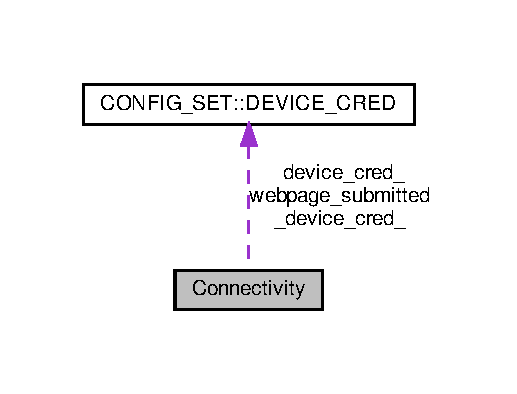
\includegraphics[width=248pt]{classConnectivity__coll__graph}
\end{center}
\end{figure}
\subsection*{Public Member Functions}
\begin{DoxyCompactItemize}
\item 
\hyperlink{classConnectivity_ad5b40b0c07375786dd882379e93df2fc}{Connectivity} (std\+::shared\+\_\+ptr$<$ \hyperlink{classLogging}{Logging} $>$ \&logging, \hyperlink{structCONFIG__SET_1_1DEVICE__CRED}{C\+O\+N\+F\+I\+G\+\_\+\+S\+E\+T\+::\+D\+E\+V\+I\+C\+E\+\_\+\+C\+R\+ED} $\ast$device\+\_\+cred)
\begin{DoxyCompactList}\small\item\em Fetches the L\+ED pin from config, setups pin mode, setup W\+S2812 R\+G\+B\+L\+ED, initializes logger. \end{DoxyCompactList}\item 
\hyperlink{classConnectivity_a0029e5f1650cb0152256d89595941e6a}{$\sim$\+Connectivity} ()
\begin{DoxyCompactList}\small\item\em Destroy the \hyperlink{classConnectivity}{Connectivity} object. \end{DoxyCompactList}\item 
void \hyperlink{classConnectivity_a08efeeef7c1096e4244224846f70f04c}{Start\+O\+TA} ()
\begin{DoxyCompactList}\small\item\em Set the up Arduino O\+TA. \end{DoxyCompactList}\item 
void \hyperlink{classConnectivity_a15482263a17c51293756870cdb516f81}{Start\+Ensure\+Connectivity} (const \hyperlink{structCONFIG__SET_1_1DEVICE__CRED}{C\+O\+N\+F\+I\+G\+\_\+\+S\+E\+T\+::\+D\+E\+V\+I\+C\+E\+\_\+\+C\+R\+ED} device\+\_\+cred)
\begin{DoxyCompactList}\small\item\em Start ensuring connectivity. \end{DoxyCompactList}\item 
int \hyperlink{classConnectivity_a8bf62c0db2251d2c9072986eae231673}{Get\+Sec\+Lost\+Connection} ()
\begin{DoxyCompactList}\small\item\em Return number of seconds of lost connection. \end{DoxyCompactList}\item 
void \hyperlink{classConnectivity_a29f2a5d6cbd259bcae65b7f7ba53b730}{Handle\+O\+TA} ()
\begin{DoxyCompactList}\small\item\em Regular call function for syncing O\+TA requests. \end{DoxyCompactList}\item 
void \hyperlink{classConnectivity_aa99aeadd725a7cd8edc7255775955807}{Stop\+O\+TA} ()
\begin{DoxyCompactList}\small\item\em Disable O\+TA. \end{DoxyCompactList}\item 
bool \hyperlink{classConnectivity_a806034c9ce5234a7fcc5370d5b6e8362}{Is\+Connected} ()
\begin{DoxyCompactList}\small\item\em Checks if the device is connected to the Wi\+Fi. \end{DoxyCompactList}\item 
void \hyperlink{classConnectivity_a72b0edad6e98830701aea73f90efd5b0}{Start\+Webpage} ()
\begin{DoxyCompactList}\small\item\em Creates a server and starts hosting webpage. \end{DoxyCompactList}\item 
void \hyperlink{classConnectivity_a5a123ddd0c4ab4061d1fa564fe3e7490}{Stop\+Webpage} ()
\begin{DoxyCompactList}\small\item\em Stops webpage server. \end{DoxyCompactList}\item 
void \hyperlink{classConnectivity_a5c562f136d52c4a91eedba957e68b71e}{Stop\+Wi\+Fi} ()
\begin{DoxyCompactList}\small\item\em disconnects Wi\+Fi \end{DoxyCompactList}\item 
std\+::tuple$<$ bool, \hyperlink{structCONFIG__SET_1_1DEVICE__CRED}{C\+O\+N\+F\+I\+G\+\_\+\+S\+E\+T\+::\+D\+E\+V\+I\+C\+E\+\_\+\+C\+R\+ED} $>$ \hyperlink{classConnectivity_a00c4168c7ac1db84abb5aa70f8f168c5}{Get\+Webpage\+Submission} ()
\begin{DoxyCompactList}\small\item\em Get the latest submission. \end{DoxyCompactList}\end{DoxyCompactItemize}
\subsection*{Private Member Functions}
\begin{DoxyCompactItemize}
\item 
void \hyperlink{classConnectivity_af7622ce70021dd32fd1ba18f62f4df62}{Start\+Hotspot} ()
\begin{DoxyCompactList}\small\item\em Starts wifi hotspot, basically start wifi in soft access point mode. \end{DoxyCompactList}\item 
void \hyperlink{classConnectivity_aaa9ca6a4b59d47cd1135101af1056a22}{Stop\+Hotspot} ()
\begin{DoxyCompactList}\small\item\em Stops wifi hotspot. \end{DoxyCompactList}\item 
void \hyperlink{classConnectivity_ac97b309654c5c550f430c5cb45850d29}{Ensure\+Connectivity} ()
\begin{DoxyCompactList}\small\item\em Check if the device is connected, if not, try to connect it. \end{DoxyCompactList}\item 
void \hyperlink{classConnectivity_a8d01492828472cc2edf8af89682b40e9}{Stop\+Ensuring\+Connectivity} ()
\begin{DoxyCompactList}\small\item\em Check if the device is connected, if not, try to connect it. \end{DoxyCompactList}\end{DoxyCompactItemize}
\subsection*{Private Attributes}
\begin{DoxyCompactItemize}
\item 
std\+::shared\+\_\+ptr$<$ \hyperlink{classLogging}{Logging} $>$ \hyperlink{classConnectivity_abc35eab84d55841433807a011e4fc934}{logger\+\_\+}
\item 
std\+::unique\+\_\+ptr$<$ Async\+Web\+Server $>$ \hyperlink{classConnectivity_a515f9aa8e3c2fae750ea2a6cd40b2d55}{webpage\+\_\+server\+\_\+} \{nullptr\}
\item 
bool \hyperlink{classConnectivity_a2aa5c1cf91cd091b26ddba14545d5dc4}{ota\+\_\+enabled\+\_\+} = false
\item 
bool \hyperlink{classConnectivity_ac43fe86c25a622135065153b1d48fd23}{webpage\+\_\+enabled\+\_\+} = false
\item 
bool \hyperlink{classConnectivity_a66be1641c52bc974aa25d8fd03c71341}{hotspot\+\_\+enabled\+\_\+} = false
\item 
bool \hyperlink{classConnectivity_aa25bae37c163e7126f3817330200f35e}{keep\+\_\+handler\+\_\+running\+\_\+} = false
\item 
bool \hyperlink{classConnectivity_aa8ebaf115b2b8163647231dd7cf5bd4a}{is\+\_\+new\+\_\+submission\+\_\+available\+\_\+} = false
\item 
\hyperlink{namespaceCONFIG__SET_a8816a22e7885d027a52bfa0d24fa9008}{C\+O\+N\+F\+I\+G\+\_\+\+S\+E\+T\+::time\+\_\+var} \hyperlink{classConnectivity_ab09df23ebb472e3c1228cf0fab6617ba}{time\+\_\+last\+\_\+connected\+\_\+}
\item 
\hyperlink{structCONFIG__SET_1_1DEVICE__CRED}{C\+O\+N\+F\+I\+G\+\_\+\+S\+E\+T\+::\+D\+E\+V\+I\+C\+E\+\_\+\+C\+R\+ED} \hyperlink{classConnectivity_a6e95d5e8ad64b301cf95a0df5ddff9a6}{webpage\+\_\+submitted\+\_\+device\+\_\+cred\+\_\+}
\item 
\hyperlink{structCONFIG__SET_1_1DEVICE__CRED}{C\+O\+N\+F\+I\+G\+\_\+\+S\+E\+T\+::\+D\+E\+V\+I\+C\+E\+\_\+\+C\+R\+ED} \hyperlink{classConnectivity_abed78a2ba39529d90841f555a81ef04a}{device\+\_\+cred\+\_\+}
\item 
std\+::unique\+\_\+ptr$<$ std\+::thread $>$ \hyperlink{classConnectivity_afb016a3f11d6d59e9e6feb3869ea5329}{ensure\+\_\+conn\+\_\+thread\+\_\+} \{nullptr\}
\item 
std\+::mutex \hyperlink{classConnectivity_aa0df63a2602190d6db2e7d7352208307}{webpage\+\_\+submission\+\_\+mutex\+\_\+}
\end{DoxyCompactItemize}


\subsection{Constructor \& Destructor Documentation}
\mbox{\Hypertarget{classConnectivity_ad5b40b0c07375786dd882379e93df2fc}\label{classConnectivity_ad5b40b0c07375786dd882379e93df2fc}} 
\index{Connectivity@{Connectivity}!Connectivity@{Connectivity}}
\index{Connectivity@{Connectivity}!Connectivity@{Connectivity}}
\subsubsection{\texorpdfstring{Connectivity()}{Connectivity()}}
{\footnotesize\ttfamily Connectivity\+::\+Connectivity (\begin{DoxyParamCaption}\item[{std\+::shared\+\_\+ptr$<$ \hyperlink{classLogging}{Logging} $>$ \&}]{logging,  }\item[{\hyperlink{structCONFIG__SET_1_1DEVICE__CRED}{C\+O\+N\+F\+I\+G\+\_\+\+S\+E\+T\+::\+D\+E\+V\+I\+C\+E\+\_\+\+C\+R\+ED} $\ast$}]{device\+\_\+cred }\end{DoxyParamCaption})}



Fetches the L\+ED pin from config, setups pin mode, setup W\+S2812 R\+G\+B\+L\+ED, initializes logger. 

\mbox{\Hypertarget{classConnectivity_a0029e5f1650cb0152256d89595941e6a}\label{classConnectivity_a0029e5f1650cb0152256d89595941e6a}} 
\index{Connectivity@{Connectivity}!````~Connectivity@{$\sim$\+Connectivity}}
\index{````~Connectivity@{$\sim$\+Connectivity}!Connectivity@{Connectivity}}
\subsubsection{\texorpdfstring{$\sim$\+Connectivity()}{~Connectivity()}}
{\footnotesize\ttfamily Connectivity\+::$\sim$\+Connectivity (\begin{DoxyParamCaption}{ }\end{DoxyParamCaption})}



Destroy the \hyperlink{classConnectivity}{Connectivity} object. 

Here is the call graph for this function\+:
\nopagebreak
\begin{figure}[H]
\begin{center}
\leavevmode
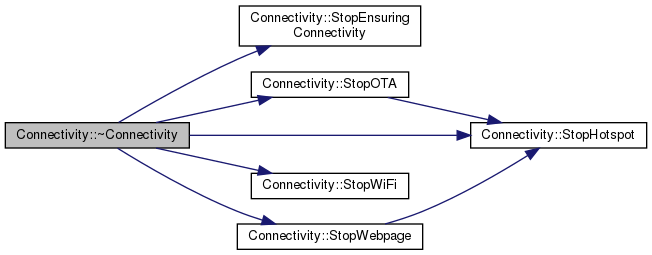
\includegraphics[width=350pt]{classConnectivity_a0029e5f1650cb0152256d89595941e6a_cgraph}
\end{center}
\end{figure}


\subsection{Member Function Documentation}
\mbox{\Hypertarget{classConnectivity_ac97b309654c5c550f430c5cb45850d29}\label{classConnectivity_ac97b309654c5c550f430c5cb45850d29}} 
\index{Connectivity@{Connectivity}!Ensure\+Connectivity@{Ensure\+Connectivity}}
\index{Ensure\+Connectivity@{Ensure\+Connectivity}!Connectivity@{Connectivity}}
\subsubsection{\texorpdfstring{Ensure\+Connectivity()}{EnsureConnectivity()}}
{\footnotesize\ttfamily void Connectivity\+::\+Ensure\+Connectivity (\begin{DoxyParamCaption}{ }\end{DoxyParamCaption})\hspace{0.3cm}{\ttfamily [private]}}



Check if the device is connected, if not, try to connect it. 

\begin{DoxyReturn}{Returns}
true \+: wifi is connected 

false \+: failed to connect, device is no longer connected, despite of trying 
\end{DoxyReturn}
Here is the call graph for this function\+:
\nopagebreak
\begin{figure}[H]
\begin{center}
\leavevmode
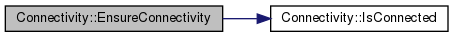
\includegraphics[width=350pt]{classConnectivity_ac97b309654c5c550f430c5cb45850d29_cgraph}
\end{center}
\end{figure}
Here is the caller graph for this function\+:
\nopagebreak
\begin{figure}[H]
\begin{center}
\leavevmode
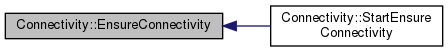
\includegraphics[width=350pt]{classConnectivity_ac97b309654c5c550f430c5cb45850d29_icgraph}
\end{center}
\end{figure}
\mbox{\Hypertarget{classConnectivity_a8bf62c0db2251d2c9072986eae231673}\label{classConnectivity_a8bf62c0db2251d2c9072986eae231673}} 
\index{Connectivity@{Connectivity}!Get\+Sec\+Lost\+Connection@{Get\+Sec\+Lost\+Connection}}
\index{Get\+Sec\+Lost\+Connection@{Get\+Sec\+Lost\+Connection}!Connectivity@{Connectivity}}
\subsubsection{\texorpdfstring{Get\+Sec\+Lost\+Connection()}{GetSecLostConnection()}}
{\footnotesize\ttfamily int Connectivity\+::\+Get\+Sec\+Lost\+Connection (\begin{DoxyParamCaption}{ }\end{DoxyParamCaption})}



Return number of seconds of lost connection. 

\mbox{\Hypertarget{classConnectivity_a00c4168c7ac1db84abb5aa70f8f168c5}\label{classConnectivity_a00c4168c7ac1db84abb5aa70f8f168c5}} 
\index{Connectivity@{Connectivity}!Get\+Webpage\+Submission@{Get\+Webpage\+Submission}}
\index{Get\+Webpage\+Submission@{Get\+Webpage\+Submission}!Connectivity@{Connectivity}}
\subsubsection{\texorpdfstring{Get\+Webpage\+Submission()}{GetWebpageSubmission()}}
{\footnotesize\ttfamily std\+::tuple$<$ bool, \hyperlink{structCONFIG__SET_1_1DEVICE__CRED}{C\+O\+N\+F\+I\+G\+\_\+\+S\+E\+T\+::\+D\+E\+V\+I\+C\+E\+\_\+\+C\+R\+ED} $>$ Connectivity\+::\+Get\+Webpage\+Submission (\begin{DoxyParamCaption}{ }\end{DoxyParamCaption})}



Get the latest submission. 

\begin{DoxyReturn}{Returns}
std\+::tuple$<$bool, C\+O\+N\+F\+I\+G\+\_\+\+S\+E\+T\+::\+D\+E\+V\+I\+C\+E\+\_\+\+C\+R\+E\+D$>$\+: bool returning if there is a new submission available, device\+\_\+cred\+: new submission 
\end{DoxyReturn}
\mbox{\Hypertarget{classConnectivity_a29f2a5d6cbd259bcae65b7f7ba53b730}\label{classConnectivity_a29f2a5d6cbd259bcae65b7f7ba53b730}} 
\index{Connectivity@{Connectivity}!Handle\+O\+TA@{Handle\+O\+TA}}
\index{Handle\+O\+TA@{Handle\+O\+TA}!Connectivity@{Connectivity}}
\subsubsection{\texorpdfstring{Handle\+O\+T\+A()}{HandleOTA()}}
{\footnotesize\ttfamily void Connectivity\+::\+Handle\+O\+TA (\begin{DoxyParamCaption}{ }\end{DoxyParamCaption})}



Regular call function for syncing O\+TA requests. 

\mbox{\Hypertarget{classConnectivity_a806034c9ce5234a7fcc5370d5b6e8362}\label{classConnectivity_a806034c9ce5234a7fcc5370d5b6e8362}} 
\index{Connectivity@{Connectivity}!Is\+Connected@{Is\+Connected}}
\index{Is\+Connected@{Is\+Connected}!Connectivity@{Connectivity}}
\subsubsection{\texorpdfstring{Is\+Connected()}{IsConnected()}}
{\footnotesize\ttfamily bool Connectivity\+::\+Is\+Connected (\begin{DoxyParamCaption}{ }\end{DoxyParamCaption})}



Checks if the device is connected to the Wi\+Fi. 

\begin{DoxyReturn}{Returns}
true \+: if connected 

false \+: otherwise 
\end{DoxyReturn}
Here is the caller graph for this function\+:
\nopagebreak
\begin{figure}[H]
\begin{center}
\leavevmode
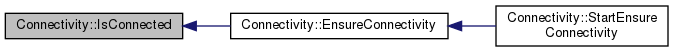
\includegraphics[width=350pt]{classConnectivity_a806034c9ce5234a7fcc5370d5b6e8362_icgraph}
\end{center}
\end{figure}
\mbox{\Hypertarget{classConnectivity_a15482263a17c51293756870cdb516f81}\label{classConnectivity_a15482263a17c51293756870cdb516f81}} 
\index{Connectivity@{Connectivity}!Start\+Ensure\+Connectivity@{Start\+Ensure\+Connectivity}}
\index{Start\+Ensure\+Connectivity@{Start\+Ensure\+Connectivity}!Connectivity@{Connectivity}}
\subsubsection{\texorpdfstring{Start\+Ensure\+Connectivity()}{StartEnsureConnectivity()}}
{\footnotesize\ttfamily void Connectivity\+::\+Start\+Ensure\+Connectivity (\begin{DoxyParamCaption}\item[{const \hyperlink{structCONFIG__SET_1_1DEVICE__CRED}{C\+O\+N\+F\+I\+G\+\_\+\+S\+E\+T\+::\+D\+E\+V\+I\+C\+E\+\_\+\+C\+R\+ED}}]{device\+\_\+cred }\end{DoxyParamCaption})}



Start ensuring connectivity. 

Here is the call graph for this function\+:
\nopagebreak
\begin{figure}[H]
\begin{center}
\leavevmode
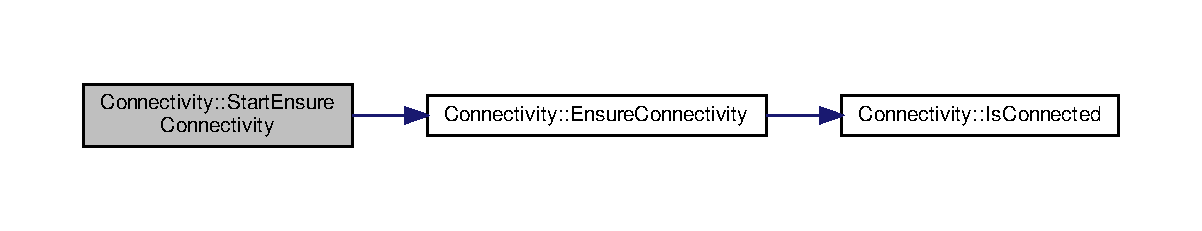
\includegraphics[width=350pt]{classConnectivity_a15482263a17c51293756870cdb516f81_cgraph}
\end{center}
\end{figure}
\mbox{\Hypertarget{classConnectivity_af7622ce70021dd32fd1ba18f62f4df62}\label{classConnectivity_af7622ce70021dd32fd1ba18f62f4df62}} 
\index{Connectivity@{Connectivity}!Start\+Hotspot@{Start\+Hotspot}}
\index{Start\+Hotspot@{Start\+Hotspot}!Connectivity@{Connectivity}}
\subsubsection{\texorpdfstring{Start\+Hotspot()}{StartHotspot()}}
{\footnotesize\ttfamily void Connectivity\+::\+Start\+Hotspot (\begin{DoxyParamCaption}{ }\end{DoxyParamCaption})\hspace{0.3cm}{\ttfamily [private]}}



Starts wifi hotspot, basically start wifi in soft access point mode. 

Here is the caller graph for this function\+:
\nopagebreak
\begin{figure}[H]
\begin{center}
\leavevmode
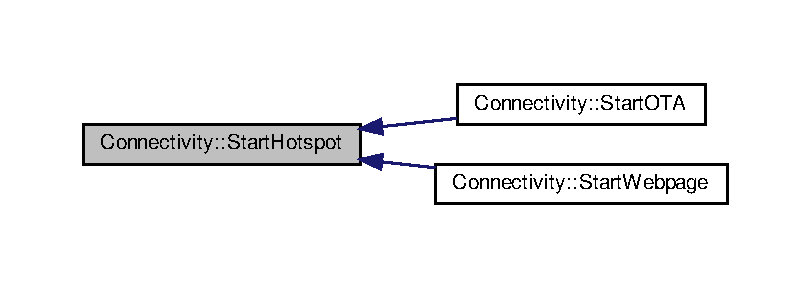
\includegraphics[width=350pt]{classConnectivity_af7622ce70021dd32fd1ba18f62f4df62_icgraph}
\end{center}
\end{figure}
\mbox{\Hypertarget{classConnectivity_a08efeeef7c1096e4244224846f70f04c}\label{classConnectivity_a08efeeef7c1096e4244224846f70f04c}} 
\index{Connectivity@{Connectivity}!Start\+O\+TA@{Start\+O\+TA}}
\index{Start\+O\+TA@{Start\+O\+TA}!Connectivity@{Connectivity}}
\subsubsection{\texorpdfstring{Start\+O\+T\+A()}{StartOTA()}}
{\footnotesize\ttfamily void Connectivity\+::\+Start\+O\+TA (\begin{DoxyParamCaption}{ }\end{DoxyParamCaption})}



Set the up Arduino O\+TA. 

Here is the call graph for this function\+:
\nopagebreak
\begin{figure}[H]
\begin{center}
\leavevmode
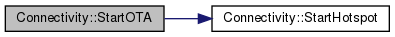
\includegraphics[width=350pt]{classConnectivity_a08efeeef7c1096e4244224846f70f04c_cgraph}
\end{center}
\end{figure}
\mbox{\Hypertarget{classConnectivity_a72b0edad6e98830701aea73f90efd5b0}\label{classConnectivity_a72b0edad6e98830701aea73f90efd5b0}} 
\index{Connectivity@{Connectivity}!Start\+Webpage@{Start\+Webpage}}
\index{Start\+Webpage@{Start\+Webpage}!Connectivity@{Connectivity}}
\subsubsection{\texorpdfstring{Start\+Webpage()}{StartWebpage()}}
{\footnotesize\ttfamily void Connectivity\+::\+Start\+Webpage (\begin{DoxyParamCaption}{ }\end{DoxyParamCaption})}



Creates a server and starts hosting webpage. 

Here is the call graph for this function\+:
\nopagebreak
\begin{figure}[H]
\begin{center}
\leavevmode
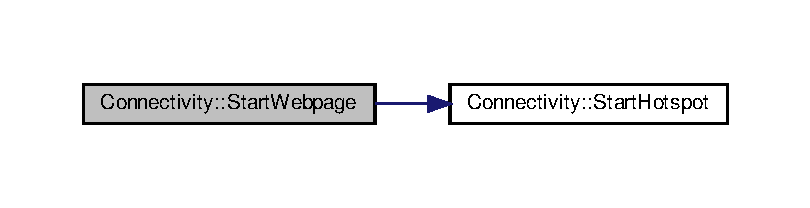
\includegraphics[width=350pt]{classConnectivity_a72b0edad6e98830701aea73f90efd5b0_cgraph}
\end{center}
\end{figure}
\mbox{\Hypertarget{classConnectivity_a8d01492828472cc2edf8af89682b40e9}\label{classConnectivity_a8d01492828472cc2edf8af89682b40e9}} 
\index{Connectivity@{Connectivity}!Stop\+Ensuring\+Connectivity@{Stop\+Ensuring\+Connectivity}}
\index{Stop\+Ensuring\+Connectivity@{Stop\+Ensuring\+Connectivity}!Connectivity@{Connectivity}}
\subsubsection{\texorpdfstring{Stop\+Ensuring\+Connectivity()}{StopEnsuringConnectivity()}}
{\footnotesize\ttfamily void Connectivity\+::\+Stop\+Ensuring\+Connectivity (\begin{DoxyParamCaption}{ }\end{DoxyParamCaption})\hspace{0.3cm}{\ttfamily [private]}}



Check if the device is connected, if not, try to connect it. 

\begin{DoxyReturn}{Returns}
true \+: wifi is connected 

false \+: failed to connect, device is no longer connected, despite of trying 
\end{DoxyReturn}
Here is the caller graph for this function\+:
\nopagebreak
\begin{figure}[H]
\begin{center}
\leavevmode
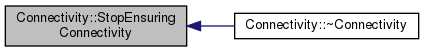
\includegraphics[width=350pt]{classConnectivity_a8d01492828472cc2edf8af89682b40e9_icgraph}
\end{center}
\end{figure}
\mbox{\Hypertarget{classConnectivity_aaa9ca6a4b59d47cd1135101af1056a22}\label{classConnectivity_aaa9ca6a4b59d47cd1135101af1056a22}} 
\index{Connectivity@{Connectivity}!Stop\+Hotspot@{Stop\+Hotspot}}
\index{Stop\+Hotspot@{Stop\+Hotspot}!Connectivity@{Connectivity}}
\subsubsection{\texorpdfstring{Stop\+Hotspot()}{StopHotspot()}}
{\footnotesize\ttfamily void Connectivity\+::\+Stop\+Hotspot (\begin{DoxyParamCaption}{ }\end{DoxyParamCaption})\hspace{0.3cm}{\ttfamily [private]}}



Stops wifi hotspot. 

Here is the caller graph for this function\+:
\nopagebreak
\begin{figure}[H]
\begin{center}
\leavevmode
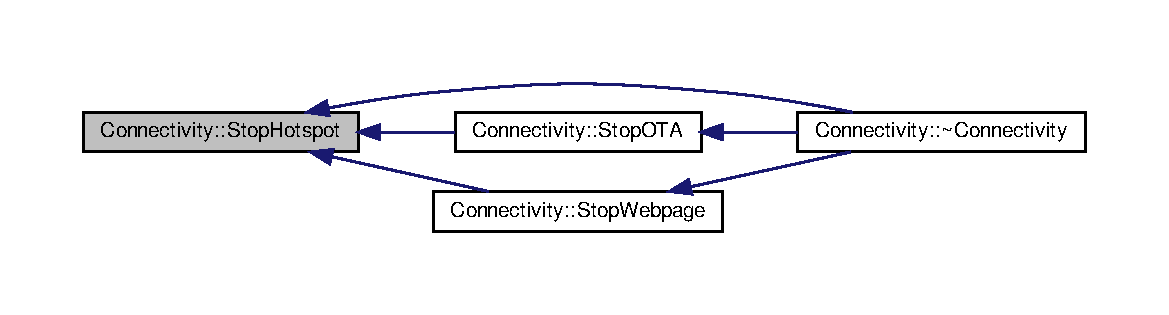
\includegraphics[width=350pt]{classConnectivity_aaa9ca6a4b59d47cd1135101af1056a22_icgraph}
\end{center}
\end{figure}
\mbox{\Hypertarget{classConnectivity_aa99aeadd725a7cd8edc7255775955807}\label{classConnectivity_aa99aeadd725a7cd8edc7255775955807}} 
\index{Connectivity@{Connectivity}!Stop\+O\+TA@{Stop\+O\+TA}}
\index{Stop\+O\+TA@{Stop\+O\+TA}!Connectivity@{Connectivity}}
\subsubsection{\texorpdfstring{Stop\+O\+T\+A()}{StopOTA()}}
{\footnotesize\ttfamily void Connectivity\+::\+Stop\+O\+TA (\begin{DoxyParamCaption}{ }\end{DoxyParamCaption})}



Disable O\+TA. 

Here is the call graph for this function\+:
\nopagebreak
\begin{figure}[H]
\begin{center}
\leavevmode
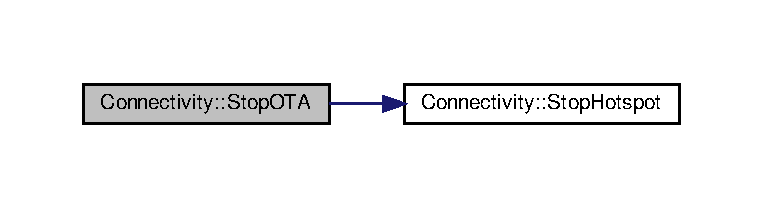
\includegraphics[width=350pt]{classConnectivity_aa99aeadd725a7cd8edc7255775955807_cgraph}
\end{center}
\end{figure}
Here is the caller graph for this function\+:
\nopagebreak
\begin{figure}[H]
\begin{center}
\leavevmode
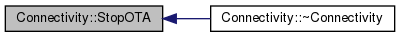
\includegraphics[width=350pt]{classConnectivity_aa99aeadd725a7cd8edc7255775955807_icgraph}
\end{center}
\end{figure}
\mbox{\Hypertarget{classConnectivity_a5a123ddd0c4ab4061d1fa564fe3e7490}\label{classConnectivity_a5a123ddd0c4ab4061d1fa564fe3e7490}} 
\index{Connectivity@{Connectivity}!Stop\+Webpage@{Stop\+Webpage}}
\index{Stop\+Webpage@{Stop\+Webpage}!Connectivity@{Connectivity}}
\subsubsection{\texorpdfstring{Stop\+Webpage()}{StopWebpage()}}
{\footnotesize\ttfamily void Connectivity\+::\+Stop\+Webpage (\begin{DoxyParamCaption}{ }\end{DoxyParamCaption})}



Stops webpage server. 

Here is the call graph for this function\+:
\nopagebreak
\begin{figure}[H]
\begin{center}
\leavevmode
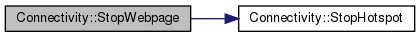
\includegraphics[width=350pt]{classConnectivity_a5a123ddd0c4ab4061d1fa564fe3e7490_cgraph}
\end{center}
\end{figure}
Here is the caller graph for this function\+:
\nopagebreak
\begin{figure}[H]
\begin{center}
\leavevmode
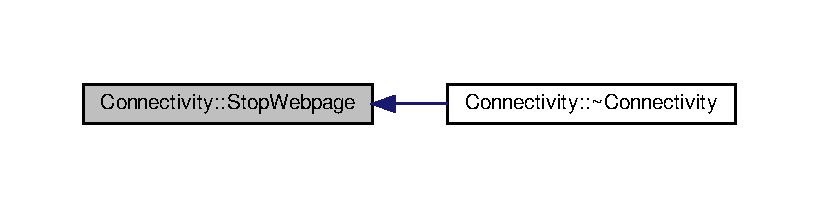
\includegraphics[width=350pt]{classConnectivity_a5a123ddd0c4ab4061d1fa564fe3e7490_icgraph}
\end{center}
\end{figure}
\mbox{\Hypertarget{classConnectivity_a5c562f136d52c4a91eedba957e68b71e}\label{classConnectivity_a5c562f136d52c4a91eedba957e68b71e}} 
\index{Connectivity@{Connectivity}!Stop\+Wi\+Fi@{Stop\+Wi\+Fi}}
\index{Stop\+Wi\+Fi@{Stop\+Wi\+Fi}!Connectivity@{Connectivity}}
\subsubsection{\texorpdfstring{Stop\+Wi\+Fi()}{StopWiFi()}}
{\footnotesize\ttfamily void Connectivity\+::\+Stop\+Wi\+Fi (\begin{DoxyParamCaption}{ }\end{DoxyParamCaption})}



disconnects Wi\+Fi 

Here is the caller graph for this function\+:
\nopagebreak
\begin{figure}[H]
\begin{center}
\leavevmode
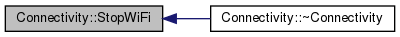
\includegraphics[width=350pt]{classConnectivity_a5c562f136d52c4a91eedba957e68b71e_icgraph}
\end{center}
\end{figure}


\subsection{Member Data Documentation}
\mbox{\Hypertarget{classConnectivity_abed78a2ba39529d90841f555a81ef04a}\label{classConnectivity_abed78a2ba39529d90841f555a81ef04a}} 
\index{Connectivity@{Connectivity}!device\+\_\+cred\+\_\+@{device\+\_\+cred\+\_\+}}
\index{device\+\_\+cred\+\_\+@{device\+\_\+cred\+\_\+}!Connectivity@{Connectivity}}
\subsubsection{\texorpdfstring{device\+\_\+cred\+\_\+}{device\_cred\_}}
{\footnotesize\ttfamily \hyperlink{structCONFIG__SET_1_1DEVICE__CRED}{C\+O\+N\+F\+I\+G\+\_\+\+S\+E\+T\+::\+D\+E\+V\+I\+C\+E\+\_\+\+C\+R\+ED} Connectivity\+::device\+\_\+cred\+\_\+\hspace{0.3cm}{\ttfamily [private]}}

\mbox{\Hypertarget{classConnectivity_afb016a3f11d6d59e9e6feb3869ea5329}\label{classConnectivity_afb016a3f11d6d59e9e6feb3869ea5329}} 
\index{Connectivity@{Connectivity}!ensure\+\_\+conn\+\_\+thread\+\_\+@{ensure\+\_\+conn\+\_\+thread\+\_\+}}
\index{ensure\+\_\+conn\+\_\+thread\+\_\+@{ensure\+\_\+conn\+\_\+thread\+\_\+}!Connectivity@{Connectivity}}
\subsubsection{\texorpdfstring{ensure\+\_\+conn\+\_\+thread\+\_\+}{ensure\_conn\_thread\_}}
{\footnotesize\ttfamily std\+::unique\+\_\+ptr$<$std\+::thread$>$ Connectivity\+::ensure\+\_\+conn\+\_\+thread\+\_\+ \{nullptr\}\hspace{0.3cm}{\ttfamily [private]}}

\mbox{\Hypertarget{classConnectivity_a66be1641c52bc974aa25d8fd03c71341}\label{classConnectivity_a66be1641c52bc974aa25d8fd03c71341}} 
\index{Connectivity@{Connectivity}!hotspot\+\_\+enabled\+\_\+@{hotspot\+\_\+enabled\+\_\+}}
\index{hotspot\+\_\+enabled\+\_\+@{hotspot\+\_\+enabled\+\_\+}!Connectivity@{Connectivity}}
\subsubsection{\texorpdfstring{hotspot\+\_\+enabled\+\_\+}{hotspot\_enabled\_}}
{\footnotesize\ttfamily bool Connectivity\+::hotspot\+\_\+enabled\+\_\+ = false\hspace{0.3cm}{\ttfamily [private]}}

\mbox{\Hypertarget{classConnectivity_aa8ebaf115b2b8163647231dd7cf5bd4a}\label{classConnectivity_aa8ebaf115b2b8163647231dd7cf5bd4a}} 
\index{Connectivity@{Connectivity}!is\+\_\+new\+\_\+submission\+\_\+available\+\_\+@{is\+\_\+new\+\_\+submission\+\_\+available\+\_\+}}
\index{is\+\_\+new\+\_\+submission\+\_\+available\+\_\+@{is\+\_\+new\+\_\+submission\+\_\+available\+\_\+}!Connectivity@{Connectivity}}
\subsubsection{\texorpdfstring{is\+\_\+new\+\_\+submission\+\_\+available\+\_\+}{is\_new\_submission\_available\_}}
{\footnotesize\ttfamily bool Connectivity\+::is\+\_\+new\+\_\+submission\+\_\+available\+\_\+ = false\hspace{0.3cm}{\ttfamily [private]}}

\mbox{\Hypertarget{classConnectivity_aa25bae37c163e7126f3817330200f35e}\label{classConnectivity_aa25bae37c163e7126f3817330200f35e}} 
\index{Connectivity@{Connectivity}!keep\+\_\+handler\+\_\+running\+\_\+@{keep\+\_\+handler\+\_\+running\+\_\+}}
\index{keep\+\_\+handler\+\_\+running\+\_\+@{keep\+\_\+handler\+\_\+running\+\_\+}!Connectivity@{Connectivity}}
\subsubsection{\texorpdfstring{keep\+\_\+handler\+\_\+running\+\_\+}{keep\_handler\_running\_}}
{\footnotesize\ttfamily bool Connectivity\+::keep\+\_\+handler\+\_\+running\+\_\+ = false\hspace{0.3cm}{\ttfamily [private]}}

\mbox{\Hypertarget{classConnectivity_abc35eab84d55841433807a011e4fc934}\label{classConnectivity_abc35eab84d55841433807a011e4fc934}} 
\index{Connectivity@{Connectivity}!logger\+\_\+@{logger\+\_\+}}
\index{logger\+\_\+@{logger\+\_\+}!Connectivity@{Connectivity}}
\subsubsection{\texorpdfstring{logger\+\_\+}{logger\_}}
{\footnotesize\ttfamily std\+::shared\+\_\+ptr$<$\hyperlink{classLogging}{Logging}$>$ Connectivity\+::logger\+\_\+\hspace{0.3cm}{\ttfamily [private]}}

\mbox{\Hypertarget{classConnectivity_a2aa5c1cf91cd091b26ddba14545d5dc4}\label{classConnectivity_a2aa5c1cf91cd091b26ddba14545d5dc4}} 
\index{Connectivity@{Connectivity}!ota\+\_\+enabled\+\_\+@{ota\+\_\+enabled\+\_\+}}
\index{ota\+\_\+enabled\+\_\+@{ota\+\_\+enabled\+\_\+}!Connectivity@{Connectivity}}
\subsubsection{\texorpdfstring{ota\+\_\+enabled\+\_\+}{ota\_enabled\_}}
{\footnotesize\ttfamily bool Connectivity\+::ota\+\_\+enabled\+\_\+ = false\hspace{0.3cm}{\ttfamily [private]}}

\mbox{\Hypertarget{classConnectivity_ab09df23ebb472e3c1228cf0fab6617ba}\label{classConnectivity_ab09df23ebb472e3c1228cf0fab6617ba}} 
\index{Connectivity@{Connectivity}!time\+\_\+last\+\_\+connected\+\_\+@{time\+\_\+last\+\_\+connected\+\_\+}}
\index{time\+\_\+last\+\_\+connected\+\_\+@{time\+\_\+last\+\_\+connected\+\_\+}!Connectivity@{Connectivity}}
\subsubsection{\texorpdfstring{time\+\_\+last\+\_\+connected\+\_\+}{time\_last\_connected\_}}
{\footnotesize\ttfamily \hyperlink{namespaceCONFIG__SET_a8816a22e7885d027a52bfa0d24fa9008}{C\+O\+N\+F\+I\+G\+\_\+\+S\+E\+T\+::time\+\_\+var} Connectivity\+::time\+\_\+last\+\_\+connected\+\_\+\hspace{0.3cm}{\ttfamily [private]}}

\mbox{\Hypertarget{classConnectivity_ac43fe86c25a622135065153b1d48fd23}\label{classConnectivity_ac43fe86c25a622135065153b1d48fd23}} 
\index{Connectivity@{Connectivity}!webpage\+\_\+enabled\+\_\+@{webpage\+\_\+enabled\+\_\+}}
\index{webpage\+\_\+enabled\+\_\+@{webpage\+\_\+enabled\+\_\+}!Connectivity@{Connectivity}}
\subsubsection{\texorpdfstring{webpage\+\_\+enabled\+\_\+}{webpage\_enabled\_}}
{\footnotesize\ttfamily bool Connectivity\+::webpage\+\_\+enabled\+\_\+ = false\hspace{0.3cm}{\ttfamily [private]}}

\mbox{\Hypertarget{classConnectivity_a515f9aa8e3c2fae750ea2a6cd40b2d55}\label{classConnectivity_a515f9aa8e3c2fae750ea2a6cd40b2d55}} 
\index{Connectivity@{Connectivity}!webpage\+\_\+server\+\_\+@{webpage\+\_\+server\+\_\+}}
\index{webpage\+\_\+server\+\_\+@{webpage\+\_\+server\+\_\+}!Connectivity@{Connectivity}}
\subsubsection{\texorpdfstring{webpage\+\_\+server\+\_\+}{webpage\_server\_}}
{\footnotesize\ttfamily std\+::unique\+\_\+ptr$<$Async\+Web\+Server$>$ Connectivity\+::webpage\+\_\+server\+\_\+ \{nullptr\}\hspace{0.3cm}{\ttfamily [private]}}

\mbox{\Hypertarget{classConnectivity_aa0df63a2602190d6db2e7d7352208307}\label{classConnectivity_aa0df63a2602190d6db2e7d7352208307}} 
\index{Connectivity@{Connectivity}!webpage\+\_\+submission\+\_\+mutex\+\_\+@{webpage\+\_\+submission\+\_\+mutex\+\_\+}}
\index{webpage\+\_\+submission\+\_\+mutex\+\_\+@{webpage\+\_\+submission\+\_\+mutex\+\_\+}!Connectivity@{Connectivity}}
\subsubsection{\texorpdfstring{webpage\+\_\+submission\+\_\+mutex\+\_\+}{webpage\_submission\_mutex\_}}
{\footnotesize\ttfamily std\+::mutex Connectivity\+::webpage\+\_\+submission\+\_\+mutex\+\_\+\hspace{0.3cm}{\ttfamily [private]}}

\mbox{\Hypertarget{classConnectivity_a6e95d5e8ad64b301cf95a0df5ddff9a6}\label{classConnectivity_a6e95d5e8ad64b301cf95a0df5ddff9a6}} 
\index{Connectivity@{Connectivity}!webpage\+\_\+submitted\+\_\+device\+\_\+cred\+\_\+@{webpage\+\_\+submitted\+\_\+device\+\_\+cred\+\_\+}}
\index{webpage\+\_\+submitted\+\_\+device\+\_\+cred\+\_\+@{webpage\+\_\+submitted\+\_\+device\+\_\+cred\+\_\+}!Connectivity@{Connectivity}}
\subsubsection{\texorpdfstring{webpage\+\_\+submitted\+\_\+device\+\_\+cred\+\_\+}{webpage\_submitted\_device\_cred\_}}
{\footnotesize\ttfamily \hyperlink{structCONFIG__SET_1_1DEVICE__CRED}{C\+O\+N\+F\+I\+G\+\_\+\+S\+E\+T\+::\+D\+E\+V\+I\+C\+E\+\_\+\+C\+R\+ED} Connectivity\+::webpage\+\_\+submitted\+\_\+device\+\_\+cred\+\_\+\hspace{0.3cm}{\ttfamily [private]}}



The documentation for this class was generated from the following files\+:\begin{DoxyCompactItemize}
\item 
mvp/src/connectivity/\hyperlink{connectivity_8h}{connectivity.\+h}\item 
mvp/src/connectivity/\hyperlink{connectivity_8cpp}{connectivity.\+cpp}\end{DoxyCompactItemize}

\hypertarget{classController}{}\section{Controller Class Reference}
\label{classController}\index{Controller@{Controller}}
\subsection*{Public Member Functions}
\begin{DoxyCompactItemize}
\item 
\mbox{\Hypertarget{classController_a95c56822d667e94b031451729ce069a9}\label{classController_a95c56822d667e94b031451729ce069a9}} 
\hyperlink{classController_a95c56822d667e94b031451729ce069a9}{Controller} ()
\begin{DoxyCompactList}\small\item\em Construct a new \hyperlink{classController}{Controller} object. \end{DoxyCompactList}\item 
\mbox{\Hypertarget{classController_a0ab87934c4f7a266cfdb86e0f36bc1b5}\label{classController_a0ab87934c4f7a266cfdb86e0f36bc1b5}} 
\hyperlink{classController_a0ab87934c4f7a266cfdb86e0f36bc1b5}{$\sim$\+Controller} ()
\begin{DoxyCompactList}\small\item\em Destroy the \hyperlink{classController}{Controller} object. \end{DoxyCompactList}\end{DoxyCompactItemize}


The documentation for this class was generated from the following file\+:\begin{DoxyCompactItemize}
\item 
/home/mahi/git/automatic\+\_\+curtain/mvp/src/controller/\hyperlink{controller_8h}{controller.\+h}\end{DoxyCompactItemize}

\hypertarget{classIndicator}{}\section{Indicator Class Reference}
\label{classIndicator}\index{Indicator@{Indicator}}
\subsection*{Public Member Functions}
\begin{DoxyCompactItemize}
\item 
\mbox{\Hypertarget{classIndicator_add29c7a02300b2e0cf35fb123692a6a6}\label{classIndicator_add29c7a02300b2e0cf35fb123692a6a6}} 
\hyperlink{classIndicator_add29c7a02300b2e0cf35fb123692a6a6}{Indicator} ()
\begin{DoxyCompactList}\small\item\em Construct a new \hyperlink{classIndicator}{Indicator} object. \end{DoxyCompactList}\item 
\mbox{\Hypertarget{classIndicator_a8099ca10ae3ae131b0423899f1abb61c}\label{classIndicator_a8099ca10ae3ae131b0423899f1abb61c}} 
\hyperlink{classIndicator_a8099ca10ae3ae131b0423899f1abb61c}{$\sim$\+Indicator} ()
\begin{DoxyCompactList}\small\item\em Destroy the \hyperlink{classIndicator}{Indicator} object. \end{DoxyCompactList}\item 
\mbox{\Hypertarget{classIndicator_abb3adf280408b88ad347fae180c10452}\label{classIndicator_abb3adf280408b88ad347fae180c10452}} 
void \hyperlink{classIndicator_abb3adf280408b88ad347fae180c10452}{test\+\_\+function} ()
\begin{DoxyCompactList}\small\item\em Hello. \end{DoxyCompactList}\end{DoxyCompactItemize}


The documentation for this class was generated from the following file\+:\begin{DoxyCompactItemize}
\item 
/home/mahi/git/automatic\+\_\+curtain/mvp/src/indicator/\hyperlink{indicator_8h}{indicator.\+h}\end{DoxyCompactItemize}

\hypertarget{classLogging}{}\section{Logging Class Reference}
\label{classLogging}\index{Logging@{Logging}}


{\ttfamily \#include $<$logging.\+h$>$}

\subsection*{Public Member Functions}
\begin{DoxyCompactItemize}
\item 
\hyperlink{classLogging_a3180cbe3cd3f25a926092066a157b884}{Logging} (bool logging\+\_\+status)
\begin{DoxyCompactList}\small\item\em Construct a new \hyperlink{classLogging}{Logging} object, initializes the serial connection. \end{DoxyCompactList}\item 
\hyperlink{classLogging_af6a0971121f5b0d9d6ebfb4e69b20a4d}{$\sim$\+Logging} ()
\begin{DoxyCompactList}\small\item\em Destroy the \hyperlink{classLogging}{Logging} object. \end{DoxyCompactList}\item 
bool \hyperlink{classLogging_abefeba86ea7c9ec93b7de22fc03a558e}{Log} (\hyperlink{namespaceCONFIG__SET_aaf9764960ee214f0eaabd2461e30e932}{C\+O\+N\+F\+I\+G\+\_\+\+S\+E\+T\+::\+L\+O\+G\+\_\+\+T\+Y\+PE} log\+\_\+type, \hyperlink{namespaceCONFIG__SET_a3c4daebec2ea4e9f6affb5b3abbeb863}{C\+O\+N\+F\+I\+G\+\_\+\+S\+E\+T\+::\+L\+O\+G\+\_\+\+C\+L\+A\+SS} log\+\_\+class, const char $\ast$message)
\begin{DoxyCompactList}\small\item\em For now, the function will just print a message on serial, it can be over wifi or just hardware serial. \end{DoxyCompactList}\item 
bool \hyperlink{classLogging_a7ad9e952d45e4b456006755beb62e9d3}{Log} (\hyperlink{namespaceCONFIG__SET_aaf9764960ee214f0eaabd2461e30e932}{C\+O\+N\+F\+I\+G\+\_\+\+S\+E\+T\+::\+L\+O\+G\+\_\+\+T\+Y\+PE} log\+\_\+type, \hyperlink{namespaceCONFIG__SET_a3c4daebec2ea4e9f6affb5b3abbeb863}{C\+O\+N\+F\+I\+G\+\_\+\+S\+E\+T\+::\+L\+O\+G\+\_\+\+C\+L\+A\+SS} log\+\_\+class, String message)
\begin{DoxyCompactList}\small\item\em For now, the function will just print a message on serial, it can be over wifi or just hardware serial. \end{DoxyCompactList}\item 
void \hyperlink{classLogging_a7eab89a46435adb76ea30a899e9658cc}{Set\+Logging\+Status} (bool status)
\begin{DoxyCompactList}\small\item\em This function enables or disables logging true\+: logging enabled false\+: logging disabled. \end{DoxyCompactList}\item 
bool \hyperlink{classLogging_a739f193cbcadcec708a6af983039759f}{Get\+Logging\+Status} ()
\begin{DoxyCompactList}\small\item\em Get the \hyperlink{classLogging}{Logging} Status object. \end{DoxyCompactList}\end{DoxyCompactItemize}
\subsection*{Private Attributes}
\begin{DoxyCompactItemize}
\item 
bool \hyperlink{classLogging_adc395a9b0a516df8528b6ef764877a58}{logging\+\_\+status\+\_\+}
\item 
std\+::mutex \hyperlink{classLogging_a9bc75091ce35d1448abf90ee07fc7ffa}{status\+\_\+mutex}
\end{DoxyCompactItemize}


\subsection{Constructor \& Destructor Documentation}
\mbox{\Hypertarget{classLogging_a3180cbe3cd3f25a926092066a157b884}\label{classLogging_a3180cbe3cd3f25a926092066a157b884}} 
\index{Logging@{Logging}!Logging@{Logging}}
\index{Logging@{Logging}!Logging@{Logging}}
\subsubsection{\texorpdfstring{Logging()}{Logging()}}
{\footnotesize\ttfamily Logging\+::\+Logging (\begin{DoxyParamCaption}\item[{bool}]{logging\+\_\+status }\end{DoxyParamCaption})}



Construct a new \hyperlink{classLogging}{Logging} object, initializes the serial connection. 

\mbox{\Hypertarget{classLogging_af6a0971121f5b0d9d6ebfb4e69b20a4d}\label{classLogging_af6a0971121f5b0d9d6ebfb4e69b20a4d}} 
\index{Logging@{Logging}!````~Logging@{$\sim$\+Logging}}
\index{````~Logging@{$\sim$\+Logging}!Logging@{Logging}}
\subsubsection{\texorpdfstring{$\sim$\+Logging()}{~Logging()}}
{\footnotesize\ttfamily Logging\+::$\sim$\+Logging (\begin{DoxyParamCaption}{ }\end{DoxyParamCaption})}



Destroy the \hyperlink{classLogging}{Logging} object. 



\subsection{Member Function Documentation}
\mbox{\Hypertarget{classLogging_a739f193cbcadcec708a6af983039759f}\label{classLogging_a739f193cbcadcec708a6af983039759f}} 
\index{Logging@{Logging}!Get\+Logging\+Status@{Get\+Logging\+Status}}
\index{Get\+Logging\+Status@{Get\+Logging\+Status}!Logging@{Logging}}
\subsubsection{\texorpdfstring{Get\+Logging\+Status()}{GetLoggingStatus()}}
{\footnotesize\ttfamily bool Logging\+::\+Get\+Logging\+Status (\begin{DoxyParamCaption}{ }\end{DoxyParamCaption})}



Get the \hyperlink{classLogging}{Logging} Status object. 

\begin{DoxyReturn}{Returns}
bool\+: logging\+\_\+status\+\_\+ 
\end{DoxyReturn}
\mbox{\Hypertarget{classLogging_abefeba86ea7c9ec93b7de22fc03a558e}\label{classLogging_abefeba86ea7c9ec93b7de22fc03a558e}} 
\index{Logging@{Logging}!Log@{Log}}
\index{Log@{Log}!Logging@{Logging}}
\subsubsection{\texorpdfstring{Log()}{Log()}\hspace{0.1cm}{\footnotesize\ttfamily [1/2]}}
{\footnotesize\ttfamily bool Logging\+::\+Log (\begin{DoxyParamCaption}\item[{\hyperlink{namespaceCONFIG__SET_aaf9764960ee214f0eaabd2461e30e932}{C\+O\+N\+F\+I\+G\+\_\+\+S\+E\+T\+::\+L\+O\+G\+\_\+\+T\+Y\+PE}}]{log\+\_\+type,  }\item[{\hyperlink{namespaceCONFIG__SET_a3c4daebec2ea4e9f6affb5b3abbeb863}{C\+O\+N\+F\+I\+G\+\_\+\+S\+E\+T\+::\+L\+O\+G\+\_\+\+C\+L\+A\+SS}}]{log\+\_\+class,  }\item[{const char $\ast$}]{message }\end{DoxyParamCaption})}



For now, the function will just print a message on serial, it can be over wifi or just hardware serial. 


\begin{DoxyParams}{Parameters}
{\em message} & \\
\hline
\end{DoxyParams}
\begin{DoxyReturn}{Returns}
true \+: if the print is successful 

false \+: otherwise 
\end{DoxyReturn}
Here is the caller graph for this function\+:
\nopagebreak
\begin{figure}[H]
\begin{center}
\leavevmode
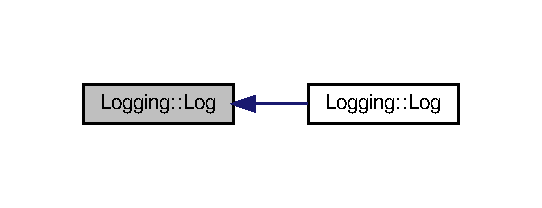
\includegraphics[width=260pt]{classLogging_abefeba86ea7c9ec93b7de22fc03a558e_icgraph}
\end{center}
\end{figure}
\mbox{\Hypertarget{classLogging_a7ad9e952d45e4b456006755beb62e9d3}\label{classLogging_a7ad9e952d45e4b456006755beb62e9d3}} 
\index{Logging@{Logging}!Log@{Log}}
\index{Log@{Log}!Logging@{Logging}}
\subsubsection{\texorpdfstring{Log()}{Log()}\hspace{0.1cm}{\footnotesize\ttfamily [2/2]}}
{\footnotesize\ttfamily bool Logging\+::\+Log (\begin{DoxyParamCaption}\item[{\hyperlink{namespaceCONFIG__SET_aaf9764960ee214f0eaabd2461e30e932}{C\+O\+N\+F\+I\+G\+\_\+\+S\+E\+T\+::\+L\+O\+G\+\_\+\+T\+Y\+PE}}]{log\+\_\+type,  }\item[{\hyperlink{namespaceCONFIG__SET_a3c4daebec2ea4e9f6affb5b3abbeb863}{C\+O\+N\+F\+I\+G\+\_\+\+S\+E\+T\+::\+L\+O\+G\+\_\+\+C\+L\+A\+SS}}]{log\+\_\+class,  }\item[{String}]{message }\end{DoxyParamCaption})}



For now, the function will just print a message on serial, it can be over wifi or just hardware serial. 


\begin{DoxyParams}{Parameters}
{\em message} & \\
\hline
\end{DoxyParams}
\begin{DoxyReturn}{Returns}
true \+: if the print is successful 

false \+: otherwise 
\end{DoxyReturn}
Here is the call graph for this function\+:
\nopagebreak
\begin{figure}[H]
\begin{center}
\leavevmode
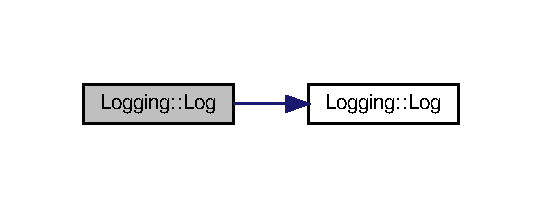
\includegraphics[width=260pt]{classLogging_a7ad9e952d45e4b456006755beb62e9d3_cgraph}
\end{center}
\end{figure}
\mbox{\Hypertarget{classLogging_a7eab89a46435adb76ea30a899e9658cc}\label{classLogging_a7eab89a46435adb76ea30a899e9658cc}} 
\index{Logging@{Logging}!Set\+Logging\+Status@{Set\+Logging\+Status}}
\index{Set\+Logging\+Status@{Set\+Logging\+Status}!Logging@{Logging}}
\subsubsection{\texorpdfstring{Set\+Logging\+Status()}{SetLoggingStatus()}}
{\footnotesize\ttfamily void Logging\+::\+Set\+Logging\+Status (\begin{DoxyParamCaption}\item[{bool}]{status }\end{DoxyParamCaption})}



This function enables or disables logging true\+: logging enabled false\+: logging disabled. 



\subsection{Member Data Documentation}
\mbox{\Hypertarget{classLogging_adc395a9b0a516df8528b6ef764877a58}\label{classLogging_adc395a9b0a516df8528b6ef764877a58}} 
\index{Logging@{Logging}!logging\+\_\+status\+\_\+@{logging\+\_\+status\+\_\+}}
\index{logging\+\_\+status\+\_\+@{logging\+\_\+status\+\_\+}!Logging@{Logging}}
\subsubsection{\texorpdfstring{logging\+\_\+status\+\_\+}{logging\_status\_}}
{\footnotesize\ttfamily bool Logging\+::logging\+\_\+status\+\_\+\hspace{0.3cm}{\ttfamily [private]}}

\mbox{\Hypertarget{classLogging_a9bc75091ce35d1448abf90ee07fc7ffa}\label{classLogging_a9bc75091ce35d1448abf90ee07fc7ffa}} 
\index{Logging@{Logging}!status\+\_\+mutex@{status\+\_\+mutex}}
\index{status\+\_\+mutex@{status\+\_\+mutex}!Logging@{Logging}}
\subsubsection{\texorpdfstring{status\+\_\+mutex}{status\_mutex}}
{\footnotesize\ttfamily std\+::mutex Logging\+::status\+\_\+mutex\hspace{0.3cm}{\ttfamily [private]}}



The documentation for this class was generated from the following files\+:\begin{DoxyCompactItemize}
\item 
mvp/src/logging/\hyperlink{logging_8h}{logging.\+h}\item 
mvp/src/logging/\hyperlink{logging_8cpp}{logging.\+cpp}\end{DoxyCompactItemize}

\hypertarget{classManualInteraction}{}\section{Manual\+Interaction Class Reference}
\label{classManualInteraction}\index{Manual\+Interaction@{Manual\+Interaction}}
\subsection*{Public Member Functions}
\begin{DoxyCompactItemize}
\item 
\mbox{\Hypertarget{classManualInteraction_a985c5461281d82a30b178376fb9c3fb3}\label{classManualInteraction_a985c5461281d82a30b178376fb9c3fb3}} 
\hyperlink{classManualInteraction_a985c5461281d82a30b178376fb9c3fb3}{Manual\+Interaction} ()
\begin{DoxyCompactList}\small\item\em Construct a new \hyperlink{classManualInteraction}{Manual\+Interaction} object. \end{DoxyCompactList}\item 
\mbox{\Hypertarget{classManualInteraction_a761406994ea72ce26d6bef061fb5ae2b}\label{classManualInteraction_a761406994ea72ce26d6bef061fb5ae2b}} 
\hyperlink{classManualInteraction_a761406994ea72ce26d6bef061fb5ae2b}{$\sim$\+Manual\+Interaction} ()
\begin{DoxyCompactList}\small\item\em Destroy the \hyperlink{classManualInteraction}{Manual\+Interaction} object. \end{DoxyCompactList}\item 
\mbox{\Hypertarget{classManualInteraction_a7782f4d4ba9d4977e253f17b7ab95198}\label{classManualInteraction_a7782f4d4ba9d4977e253f17b7ab95198}} 
void \hyperlink{classManualInteraction_a7782f4d4ba9d4977e253f17b7ab95198}{test\+\_\+function} ()
\begin{DoxyCompactList}\small\item\em Hello. \end{DoxyCompactList}\end{DoxyCompactItemize}


The documentation for this class was generated from the following file\+:\begin{DoxyCompactItemize}
\item 
/home/mahi/git/automatic\+\_\+curtain/mvp/src/manual\+\_\+interaction/\hyperlink{manual__interaction_8h}{manual\+\_\+interaction.\+h}\end{DoxyCompactItemize}

\hypertarget{classMotorDriver}{}\section{Motor\+Driver Class Reference}
\label{classMotorDriver}\index{Motor\+Driver@{Motor\+Driver}}


{\ttfamily \#include $<$motor\+\_\+driver.\+h$>$}



Inheritance diagram for Motor\+Driver\+:
\nopagebreak
\begin{figure}[H]
\begin{center}
\leavevmode
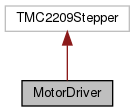
\includegraphics[width=173pt]{classMotorDriver__inherit__graph}
\end{center}
\end{figure}


Collaboration diagram for Motor\+Driver\+:
\nopagebreak
\begin{figure}[H]
\begin{center}
\leavevmode
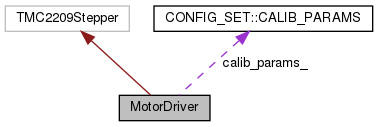
\includegraphics[width=350pt]{classMotorDriver__coll__graph}
\end{center}
\end{figure}
\subsection*{Public Member Functions}
\begin{DoxyCompactItemize}
\item 
\hyperlink{classMotorDriver_ac03c1c5c2ac455e46fe196881641b366}{Motor\+Driver} (std\+::shared\+\_\+ptr$<$ \hyperlink{classLogging}{Logging} $>$ \&logging)
\begin{DoxyCompactList}\small\item\em Initializes motor drive T\+M\+C2209, and required pins. \end{DoxyCompactList}\item 
\hyperlink{classMotorDriver_a534f4ca22b5dcffc9e40aafef09c76e5}{Motor\+Driver} (std\+::shared\+\_\+ptr$<$ \hyperlink{classLogging}{Logging} $>$ \&logging, \hyperlink{structCONFIG__SET_1_1CALIB__PARAMS}{C\+O\+N\+F\+I\+G\+\_\+\+S\+E\+T\+::\+C\+A\+L\+I\+B\+\_\+\+P\+A\+R\+A\+MS} calib\+\_\+param)
\begin{DoxyCompactList}\small\item\em Initializes motor drive T\+M\+C2209, and required pins. \end{DoxyCompactList}\item 
\hyperlink{classMotorDriver_a6ead9d8f796501adf9889a8e5aa7afc5}{$\sim$\+Motor\+Driver} ()
\begin{DoxyCompactList}\small\item\em Cleans and disables motor driver. \end{DoxyCompactList}\item 
\hyperlink{namespaceCONFIG__SET_a722f4ba49e35faf1a2504aa23677b2f0}{C\+O\+N\+F\+I\+G\+\_\+\+S\+E\+T\+::\+D\+R\+I\+V\+E\+R\+\_\+\+S\+T\+A\+T\+US} \hyperlink{classMotorDriver_a1a33492e58ce3c13cd3c090c704b1734}{Get\+Status} ()
\begin{DoxyCompactList}\small\item\em Returns the status of the motor driver, by checking if the motor is running or the driver is in fault, or the motor is available for next request. \end{DoxyCompactList}\item 
int \hyperlink{classMotorDriver_aaf134c97d67e0ce422853cc1cb7684a9}{Get\+Steps} ()
\begin{DoxyCompactList}\small\item\em Returns the current steps of motor. \end{DoxyCompactList}\item 
int \hyperlink{classMotorDriver_a409447a5b649f11549d4c6764a304d11}{Get\+Percentage} ()
\begin{DoxyCompactList}\small\item\em Returns the current percentage of motor. \end{DoxyCompactList}\item 
bool \hyperlink{classMotorDriver_a47d4e4a6cd3eec255eee3864a45e7e76}{Fulfill\+Request} (\hyperlink{structCONFIG__SET_1_1MOTION__REQUEST}{C\+O\+N\+F\+I\+G\+\_\+\+S\+E\+T\+::\+M\+O\+T\+I\+O\+N\+\_\+\+R\+E\+Q\+U\+E\+ST} request)
\begin{DoxyCompactList}\small\item\em This is the primary contact function for external requests, it will handle all requests from the controller or anywhere else, run the thread for supplying steps. \end{DoxyCompactList}\item 
bool \hyperlink{classMotorDriver_af1a7f20e03d76a0c1dac5e2080edd832}{Cancel\+Current\+Request} ()
\begin{DoxyCompactList}\small\item\em Cancels current request. \end{DoxyCompactList}\item 
void \hyperlink{classMotorDriver_a04e97c6adc4df4d186d6799dfd8165b2}{Update\+Calib\+Params} (\hyperlink{structCONFIG__SET_1_1CALIB__PARAMS}{C\+O\+N\+F\+I\+G\+\_\+\+S\+E\+T\+::\+C\+A\+L\+I\+B\+\_\+\+P\+A\+R\+A\+MS} calib\+\_\+param)
\begin{DoxyCompactList}\small\item\em Updates calibration parameters to be used by motor driver. \end{DoxyCompactList}\item 
void \hyperlink{classMotorDriver_a43c47b4f550a3ee08e7da340e699ba76}{Stop\+Handler} ()
\begin{DoxyCompactList}\small\item\em Stop handler thread. \end{DoxyCompactList}\end{DoxyCompactItemize}
\subsection*{Static Public Member Functions}
\begin{DoxyCompactItemize}
\item 
static void \hyperlink{classMotorDriver_a74f208c889afd6ed5cf5008fbb0fdb63}{Interrupt\+For\+Index} ()
\begin{DoxyCompactList}\small\item\em Runs on a timer, supplies step and direction signal to motor driver. \end{DoxyCompactList}\end{DoxyCompactItemize}
\subsection*{Private Member Functions}
\begin{DoxyCompactItemize}
\item 
void \hyperlink{classMotorDriver_a1eee734aa12c1565d6ae629924962115}{Handler} ()
\begin{DoxyCompactList}\small\item\em Motor Driver class handler, communicates with driver and is responsible for reading latest motion request, cancellationof request, and acting upon it i.\+e. moving the motor and stopping it when stall is detected, or motor reached destination or stop is requested or timer limit is reached. \end{DoxyCompactList}\item 
bool \hyperlink{classMotorDriver_a754252fe0d18118e074cbdc1fe42da57}{Enable\+Driver} (bool enable)
\begin{DoxyCompactList}\small\item\em Enable Motor Driver Give argument as true for enabling, false for disabling the driver. \end{DoxyCompactList}\item 
void \hyperlink{classMotorDriver_a9151c6649515b7ff61dc6159456ffa80}{Initialize\+Driver} ()
\begin{DoxyCompactList}\small\item\em Sets needed parameters for the driver. \end{DoxyCompactList}\item 
void \hyperlink{classMotorDriver_a5ebab90ca98fa04463de1cbae76af994}{Start\+Motor} ()
\begin{DoxyCompactList}\small\item\em Responsible for starting the motor, i.\+e. setups the driver and sets required velocity of motor. \end{DoxyCompactList}\item 
void \hyperlink{classMotorDriver_aff8659e64841fb4b97c23b3494cd0575}{Stop\+Motor} ()
\begin{DoxyCompactList}\small\item\em Responsible for stopping the motor, i.\+e. disables the driver and sets velocity of motor to zero. \end{DoxyCompactList}\item 
void \hyperlink{classMotorDriver_a64827491330490668bb8f8e57d0f3942}{Start\+Handler} ()
\begin{DoxyCompactList}\small\item\em Starts handler thread. \end{DoxyCompactList}\item 
void \hyperlink{classMotorDriver_a19833e114feff56c3a7d1d032a455e0a}{Reset\+Steps} ()
\begin{DoxyCompactList}\small\item\em Reset the current steps of motor. \end{DoxyCompactList}\end{DoxyCompactItemize}
\subsection*{Private Attributes}
\begin{DoxyCompactItemize}
\item 
\hyperlink{namespaceCONFIG__SET_a722f4ba49e35faf1a2504aa23677b2f0}{C\+O\+N\+F\+I\+G\+\_\+\+S\+E\+T\+::\+D\+R\+I\+V\+E\+R\+\_\+\+S\+T\+A\+T\+US} \hyperlink{classMotorDriver_ad99c6f2f224f78428b137f7856cfba4b}{driver\+\_\+status\+\_\+}
\item 
\hyperlink{structCONFIG__SET_1_1CALIB__PARAMS}{C\+O\+N\+F\+I\+G\+\_\+\+S\+E\+T\+::\+C\+A\+L\+I\+B\+\_\+\+P\+A\+R\+A\+MS} \hyperlink{classMotorDriver_aa2d3e952c7708106df0c86196490a499}{calib\+\_\+params\+\_\+}
\item 
std\+::shared\+\_\+ptr$<$ \hyperlink{classLogging}{Logging} $>$ \hyperlink{classMotorDriver_a6c443fae635cf2b50bfa205ac4f6418e}{logger\+\_\+}
\item 
bool \hyperlink{classMotorDriver_abbc66ce217161de9ed45003718cd6c0e}{is\+\_\+motor\+\_\+running\+\_\+} = false
\item 
hw\+\_\+timer\+\_\+t $\ast$ \hyperlink{classMotorDriver_a86d3f7015a61c62463ea3e718c5bba1c}{step\+\_\+timer\+\_\+} = N\+U\+LL
\item 
int \hyperlink{classMotorDriver_a140b9b922847586721725b7e76943c1e}{expected\+\_\+step\+\_\+} = 0
\item 
bool \hyperlink{classMotorDriver_acc772188969ac8c859d1e9c800eb0076}{blind\+\_\+traversal\+\_\+requested\+\_\+} = false
\item 
bool \hyperlink{classMotorDriver_a6c190777a6bcad1ea12f73707ed67de9}{stop\+\_\+requested\+\_\+} = false
\item 
bool \hyperlink{classMotorDriver_a930d873aa0a5961bd49b8b68553f5044}{keep\+\_\+handler\+\_\+running\+\_\+} = false
\item 
std\+::time\+\_\+t \hyperlink{classMotorDriver_a938712bd2b784e0db660fdb30ad312af}{last\+\_\+motor\+\_\+start\+\_\+time\+\_\+sec\+\_\+} = std\+::time(nullptr)
\item 
std\+::unique\+\_\+ptr$<$ std\+::thread $>$ \hyperlink{classMotorDriver_aec36906063e5e09d5bb7f7843f526874}{handler\+\_\+thread\+\_\+} \{nullptr\}
\end{DoxyCompactItemize}
\subsection*{Static Private Attributes}
\begin{DoxyCompactItemize}
\item 
static int \hyperlink{classMotorDriver_ab49b3ca9359af0016c206960887349b1}{full\+\_\+rot\+\_\+step\+\_\+count\+\_\+} = (4 $\ast$ \hyperlink{namespaceCONFIG__SET_a7028034ed96d5ef10a87d1cdc12c5d27}{C\+O\+N\+F\+I\+G\+\_\+\+S\+E\+T\+::\+M\+O\+T\+O\+R\+\_\+\+D\+R\+I\+V\+E\+R\+\_\+\+M\+I\+C\+R\+O\+S\+T\+EP})
\item 
static int \hyperlink{classMotorDriver_a9072fc26381b16a6a5e39ab1d7ed1e46}{current\+\_\+step\+\_\+} = 0
\item 
static bool \hyperlink{classMotorDriver_a09cb1d904ff0b9ce54f17fa54aec8c70}{direction\+\_\+} = false
\end{DoxyCompactItemize}


\subsection{Constructor \& Destructor Documentation}
\mbox{\Hypertarget{classMotorDriver_ac03c1c5c2ac455e46fe196881641b366}\label{classMotorDriver_ac03c1c5c2ac455e46fe196881641b366}} 
\index{Motor\+Driver@{Motor\+Driver}!Motor\+Driver@{Motor\+Driver}}
\index{Motor\+Driver@{Motor\+Driver}!Motor\+Driver@{Motor\+Driver}}
\subsubsection{\texorpdfstring{Motor\+Driver()}{MotorDriver()}\hspace{0.1cm}{\footnotesize\ttfamily [1/2]}}
{\footnotesize\ttfamily Motor\+Driver\+::\+Motor\+Driver (\begin{DoxyParamCaption}\item[{std\+::shared\+\_\+ptr$<$ \hyperlink{classLogging}{Logging} $>$ \&}]{logging }\end{DoxyParamCaption})}



Initializes motor drive T\+M\+C2209, and required pins. 

\mbox{\Hypertarget{classMotorDriver_a534f4ca22b5dcffc9e40aafef09c76e5}\label{classMotorDriver_a534f4ca22b5dcffc9e40aafef09c76e5}} 
\index{Motor\+Driver@{Motor\+Driver}!Motor\+Driver@{Motor\+Driver}}
\index{Motor\+Driver@{Motor\+Driver}!Motor\+Driver@{Motor\+Driver}}
\subsubsection{\texorpdfstring{Motor\+Driver()}{MotorDriver()}\hspace{0.1cm}{\footnotesize\ttfamily [2/2]}}
{\footnotesize\ttfamily Motor\+Driver\+::\+Motor\+Driver (\begin{DoxyParamCaption}\item[{std\+::shared\+\_\+ptr$<$ \hyperlink{classLogging}{Logging} $>$ \&}]{logging,  }\item[{\hyperlink{structCONFIG__SET_1_1CALIB__PARAMS}{C\+O\+N\+F\+I\+G\+\_\+\+S\+E\+T\+::\+C\+A\+L\+I\+B\+\_\+\+P\+A\+R\+A\+MS}}]{calib\+\_\+param }\end{DoxyParamCaption})}



Initializes motor drive T\+M\+C2209, and required pins. 

Here is the call graph for this function\+:
\nopagebreak
\begin{figure}[H]
\begin{center}
\leavevmode
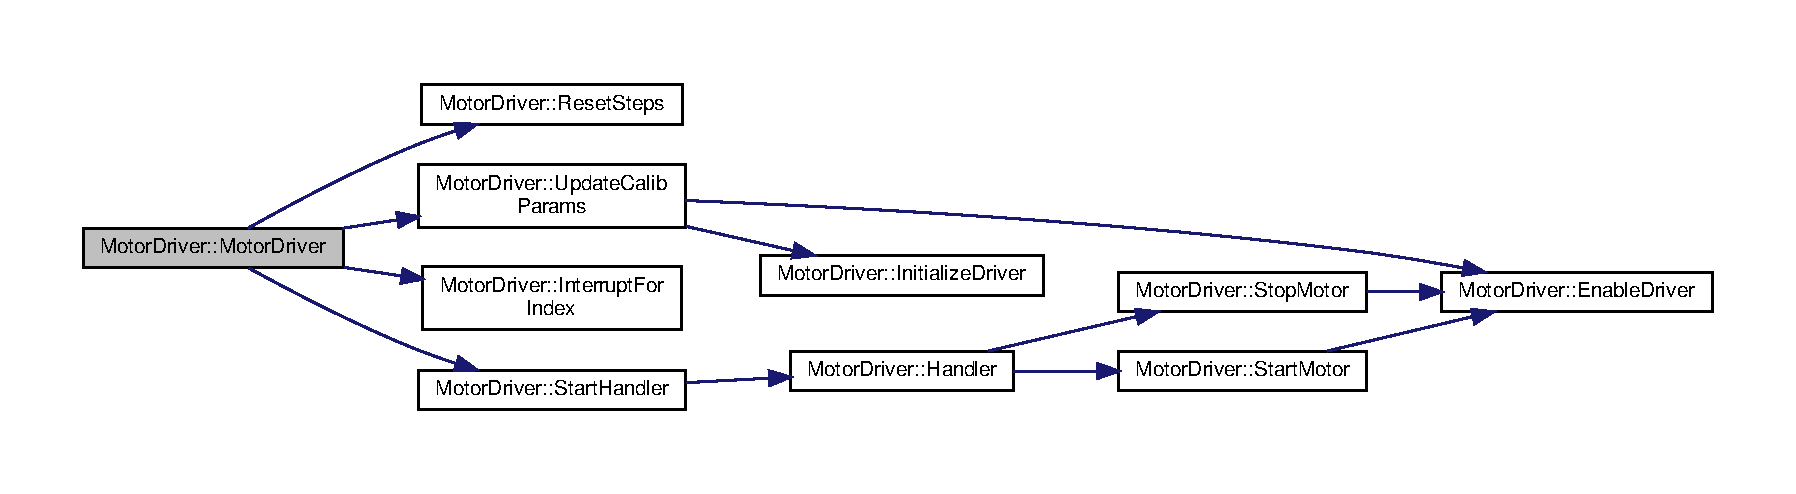
\includegraphics[width=350pt]{classMotorDriver_a534f4ca22b5dcffc9e40aafef09c76e5_cgraph}
\end{center}
\end{figure}
\mbox{\Hypertarget{classMotorDriver_a6ead9d8f796501adf9889a8e5aa7afc5}\label{classMotorDriver_a6ead9d8f796501adf9889a8e5aa7afc5}} 
\index{Motor\+Driver@{Motor\+Driver}!````~Motor\+Driver@{$\sim$\+Motor\+Driver}}
\index{````~Motor\+Driver@{$\sim$\+Motor\+Driver}!Motor\+Driver@{Motor\+Driver}}
\subsubsection{\texorpdfstring{$\sim$\+Motor\+Driver()}{~MotorDriver()}}
{\footnotesize\ttfamily Motor\+Driver\+::$\sim$\+Motor\+Driver (\begin{DoxyParamCaption}{ }\end{DoxyParamCaption})}



Cleans and disables motor driver. 

Here is the call graph for this function\+:
\nopagebreak
\begin{figure}[H]
\begin{center}
\leavevmode
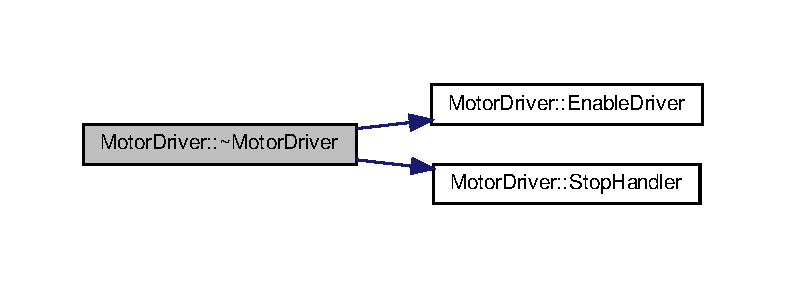
\includegraphics[width=350pt]{classMotorDriver_a6ead9d8f796501adf9889a8e5aa7afc5_cgraph}
\end{center}
\end{figure}


\subsection{Member Function Documentation}
\mbox{\Hypertarget{classMotorDriver_af1a7f20e03d76a0c1dac5e2080edd832}\label{classMotorDriver_af1a7f20e03d76a0c1dac5e2080edd832}} 
\index{Motor\+Driver@{Motor\+Driver}!Cancel\+Current\+Request@{Cancel\+Current\+Request}}
\index{Cancel\+Current\+Request@{Cancel\+Current\+Request}!Motor\+Driver@{Motor\+Driver}}
\subsubsection{\texorpdfstring{Cancel\+Current\+Request()}{CancelCurrentRequest()}}
{\footnotesize\ttfamily bool Motor\+Driver\+::\+Cancel\+Current\+Request (\begin{DoxyParamCaption}{ }\end{DoxyParamCaption})}



Cancels current request. 

\begin{DoxyReturn}{Returns}
true\+: Cancellation successful 

false\+: otherwise 
\end{DoxyReturn}
\mbox{\Hypertarget{classMotorDriver_a754252fe0d18118e074cbdc1fe42da57}\label{classMotorDriver_a754252fe0d18118e074cbdc1fe42da57}} 
\index{Motor\+Driver@{Motor\+Driver}!Enable\+Driver@{Enable\+Driver}}
\index{Enable\+Driver@{Enable\+Driver}!Motor\+Driver@{Motor\+Driver}}
\subsubsection{\texorpdfstring{Enable\+Driver()}{EnableDriver()}}
{\footnotesize\ttfamily bool Motor\+Driver\+::\+Enable\+Driver (\begin{DoxyParamCaption}\item[{bool}]{enable }\end{DoxyParamCaption})\hspace{0.3cm}{\ttfamily [private]}}



Enable Motor Driver Give argument as true for enabling, false for disabling the driver. 

\begin{DoxyReturn}{Returns}
true \+: if successful 

false \+: otherwise 
\end{DoxyReturn}
Here is the caller graph for this function\+:
\nopagebreak
\begin{figure}[H]
\begin{center}
\leavevmode
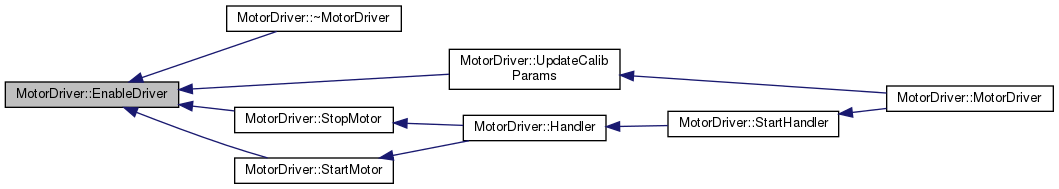
\includegraphics[width=350pt]{classMotorDriver_a754252fe0d18118e074cbdc1fe42da57_icgraph}
\end{center}
\end{figure}
\mbox{\Hypertarget{classMotorDriver_a47d4e4a6cd3eec255eee3864a45e7e76}\label{classMotorDriver_a47d4e4a6cd3eec255eee3864a45e7e76}} 
\index{Motor\+Driver@{Motor\+Driver}!Fulfill\+Request@{Fulfill\+Request}}
\index{Fulfill\+Request@{Fulfill\+Request}!Motor\+Driver@{Motor\+Driver}}
\subsubsection{\texorpdfstring{Fulfill\+Request()}{FulfillRequest()}}
{\footnotesize\ttfamily bool Motor\+Driver\+::\+Fulfill\+Request (\begin{DoxyParamCaption}\item[{\hyperlink{structCONFIG__SET_1_1MOTION__REQUEST}{C\+O\+N\+F\+I\+G\+\_\+\+S\+E\+T\+::\+M\+O\+T\+I\+O\+N\+\_\+\+R\+E\+Q\+U\+E\+ST}}]{request }\end{DoxyParamCaption})}



This is the primary contact function for external requests, it will handle all requests from the controller or anywhere else, run the thread for supplying steps. 

\begin{DoxyReturn}{Returns}
true \+: request accepted 

false \+: rejected 
\end{DoxyReturn}
\mbox{\Hypertarget{classMotorDriver_a409447a5b649f11549d4c6764a304d11}\label{classMotorDriver_a409447a5b649f11549d4c6764a304d11}} 
\index{Motor\+Driver@{Motor\+Driver}!Get\+Percentage@{Get\+Percentage}}
\index{Get\+Percentage@{Get\+Percentage}!Motor\+Driver@{Motor\+Driver}}
\subsubsection{\texorpdfstring{Get\+Percentage()}{GetPercentage()}}
{\footnotesize\ttfamily int Motor\+Driver\+::\+Get\+Percentage (\begin{DoxyParamCaption}{ }\end{DoxyParamCaption})}



Returns the current percentage of motor. 

\begin{DoxyReturn}{Returns}
current percentage 
\end{DoxyReturn}
\mbox{\Hypertarget{classMotorDriver_a1a33492e58ce3c13cd3c090c704b1734}\label{classMotorDriver_a1a33492e58ce3c13cd3c090c704b1734}} 
\index{Motor\+Driver@{Motor\+Driver}!Get\+Status@{Get\+Status}}
\index{Get\+Status@{Get\+Status}!Motor\+Driver@{Motor\+Driver}}
\subsubsection{\texorpdfstring{Get\+Status()}{GetStatus()}}
{\footnotesize\ttfamily \hyperlink{namespaceCONFIG__SET_a722f4ba49e35faf1a2504aa23677b2f0}{C\+O\+N\+F\+I\+G\+\_\+\+S\+E\+T\+::\+D\+R\+I\+V\+E\+R\+\_\+\+S\+T\+A\+T\+US} Motor\+Driver\+::\+Get\+Status (\begin{DoxyParamCaption}{ }\end{DoxyParamCaption})}



Returns the status of the motor driver, by checking if the motor is running or the driver is in fault, or the motor is available for next request. 

\begin{DoxyReturn}{Returns}
\hyperlink{namespaceCONFIG__SET_a722f4ba49e35faf1a2504aa23677b2f0}{C\+O\+N\+F\+I\+G\+\_\+\+S\+E\+T\+::\+D\+R\+I\+V\+E\+R\+\_\+\+S\+T\+A\+T\+US} 
\end{DoxyReturn}
\mbox{\Hypertarget{classMotorDriver_aaf134c97d67e0ce422853cc1cb7684a9}\label{classMotorDriver_aaf134c97d67e0ce422853cc1cb7684a9}} 
\index{Motor\+Driver@{Motor\+Driver}!Get\+Steps@{Get\+Steps}}
\index{Get\+Steps@{Get\+Steps}!Motor\+Driver@{Motor\+Driver}}
\subsubsection{\texorpdfstring{Get\+Steps()}{GetSteps()}}
{\footnotesize\ttfamily int Motor\+Driver\+::\+Get\+Steps (\begin{DoxyParamCaption}{ }\end{DoxyParamCaption})}



Returns the current steps of motor. 

\begin{DoxyReturn}{Returns}
current\+\_\+steps 
\end{DoxyReturn}
\mbox{\Hypertarget{classMotorDriver_a1eee734aa12c1565d6ae629924962115}\label{classMotorDriver_a1eee734aa12c1565d6ae629924962115}} 
\index{Motor\+Driver@{Motor\+Driver}!Handler@{Handler}}
\index{Handler@{Handler}!Motor\+Driver@{Motor\+Driver}}
\subsubsection{\texorpdfstring{Handler()}{Handler()}}
{\footnotesize\ttfamily void Motor\+Driver\+::\+Handler (\begin{DoxyParamCaption}{ }\end{DoxyParamCaption})\hspace{0.3cm}{\ttfamily [private]}}



Motor Driver class handler, communicates with driver and is responsible for reading latest motion request, cancellationof request, and acting upon it i.\+e. moving the motor and stopping it when stall is detected, or motor reached destination or stop is requested or timer limit is reached. 

Here is the call graph for this function\+:
\nopagebreak
\begin{figure}[H]
\begin{center}
\leavevmode
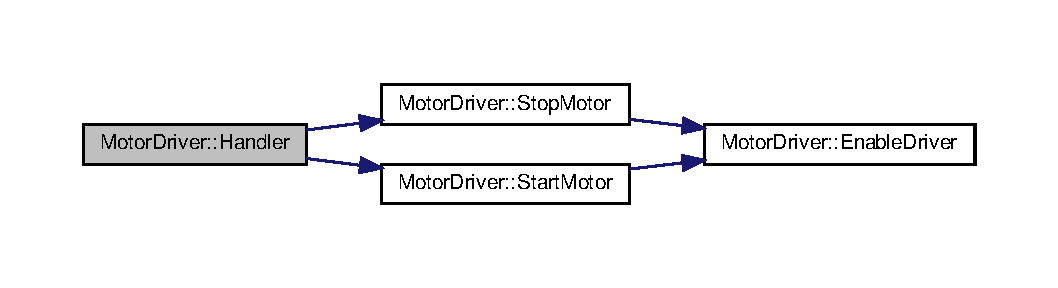
\includegraphics[width=350pt]{classMotorDriver_a1eee734aa12c1565d6ae629924962115_cgraph}
\end{center}
\end{figure}
Here is the caller graph for this function\+:
\nopagebreak
\begin{figure}[H]
\begin{center}
\leavevmode
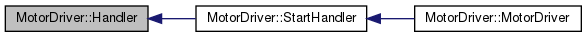
\includegraphics[width=350pt]{classMotorDriver_a1eee734aa12c1565d6ae629924962115_icgraph}
\end{center}
\end{figure}
\mbox{\Hypertarget{classMotorDriver_a9151c6649515b7ff61dc6159456ffa80}\label{classMotorDriver_a9151c6649515b7ff61dc6159456ffa80}} 
\index{Motor\+Driver@{Motor\+Driver}!Initialize\+Driver@{Initialize\+Driver}}
\index{Initialize\+Driver@{Initialize\+Driver}!Motor\+Driver@{Motor\+Driver}}
\subsubsection{\texorpdfstring{Initialize\+Driver()}{InitializeDriver()}}
{\footnotesize\ttfamily void Motor\+Driver\+::\+Initialize\+Driver (\begin{DoxyParamCaption}{ }\end{DoxyParamCaption})\hspace{0.3cm}{\ttfamily [private]}}



Sets needed parameters for the driver. 

Here is the caller graph for this function\+:
\nopagebreak
\begin{figure}[H]
\begin{center}
\leavevmode
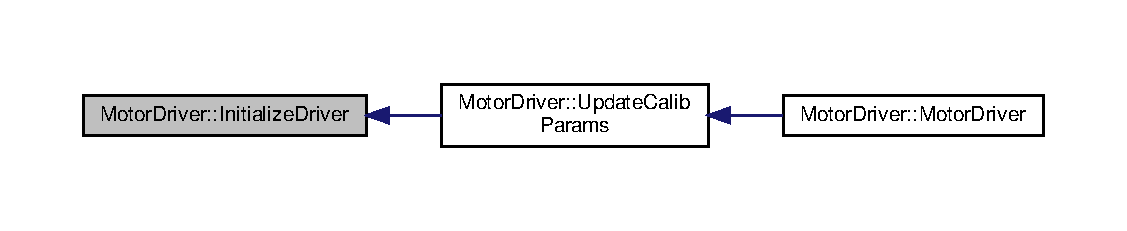
\includegraphics[width=350pt]{classMotorDriver_a9151c6649515b7ff61dc6159456ffa80_icgraph}
\end{center}
\end{figure}
\mbox{\Hypertarget{classMotorDriver_a74f208c889afd6ed5cf5008fbb0fdb63}\label{classMotorDriver_a74f208c889afd6ed5cf5008fbb0fdb63}} 
\index{Motor\+Driver@{Motor\+Driver}!Interrupt\+For\+Index@{Interrupt\+For\+Index}}
\index{Interrupt\+For\+Index@{Interrupt\+For\+Index}!Motor\+Driver@{Motor\+Driver}}
\subsubsection{\texorpdfstring{Interrupt\+For\+Index()}{InterruptForIndex()}}
{\footnotesize\ttfamily void I\+R\+A\+M\+\_\+\+A\+T\+TR Motor\+Driver\+::\+Interrupt\+For\+Index (\begin{DoxyParamCaption}{ }\end{DoxyParamCaption})\hspace{0.3cm}{\ttfamily [static]}}



Runs on a timer, supplies step and direction signal to motor driver. 

Here is the caller graph for this function\+:
\nopagebreak
\begin{figure}[H]
\begin{center}
\leavevmode
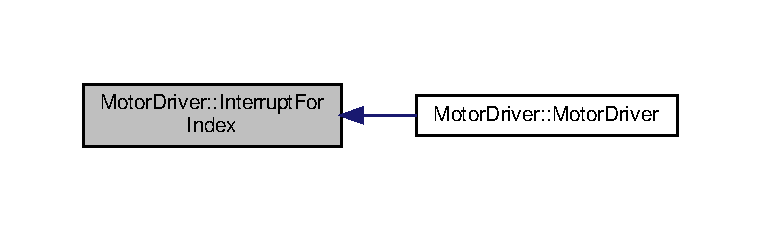
\includegraphics[width=350pt]{classMotorDriver_a74f208c889afd6ed5cf5008fbb0fdb63_icgraph}
\end{center}
\end{figure}
\mbox{\Hypertarget{classMotorDriver_a19833e114feff56c3a7d1d032a455e0a}\label{classMotorDriver_a19833e114feff56c3a7d1d032a455e0a}} 
\index{Motor\+Driver@{Motor\+Driver}!Reset\+Steps@{Reset\+Steps}}
\index{Reset\+Steps@{Reset\+Steps}!Motor\+Driver@{Motor\+Driver}}
\subsubsection{\texorpdfstring{Reset\+Steps()}{ResetSteps()}}
{\footnotesize\ttfamily void Motor\+Driver\+::\+Reset\+Steps (\begin{DoxyParamCaption}{ }\end{DoxyParamCaption})\hspace{0.3cm}{\ttfamily [private]}}



Reset the current steps of motor. 

Here is the caller graph for this function\+:
\nopagebreak
\begin{figure}[H]
\begin{center}
\leavevmode
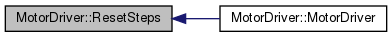
\includegraphics[width=350pt]{classMotorDriver_a19833e114feff56c3a7d1d032a455e0a_icgraph}
\end{center}
\end{figure}
\mbox{\Hypertarget{classMotorDriver_a64827491330490668bb8f8e57d0f3942}\label{classMotorDriver_a64827491330490668bb8f8e57d0f3942}} 
\index{Motor\+Driver@{Motor\+Driver}!Start\+Handler@{Start\+Handler}}
\index{Start\+Handler@{Start\+Handler}!Motor\+Driver@{Motor\+Driver}}
\subsubsection{\texorpdfstring{Start\+Handler()}{StartHandler()}}
{\footnotesize\ttfamily void Motor\+Driver\+::\+Start\+Handler (\begin{DoxyParamCaption}{ }\end{DoxyParamCaption})\hspace{0.3cm}{\ttfamily [private]}}



Starts handler thread. 

Here is the call graph for this function\+:
\nopagebreak
\begin{figure}[H]
\begin{center}
\leavevmode
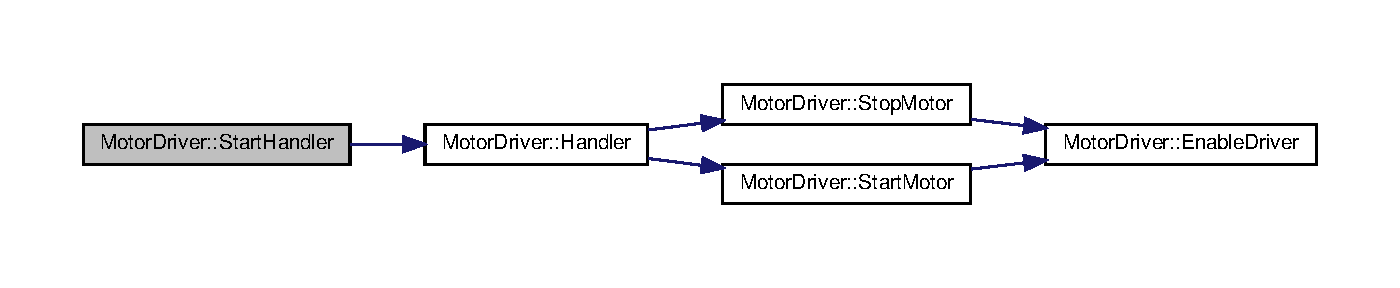
\includegraphics[width=350pt]{classMotorDriver_a64827491330490668bb8f8e57d0f3942_cgraph}
\end{center}
\end{figure}
Here is the caller graph for this function\+:
\nopagebreak
\begin{figure}[H]
\begin{center}
\leavevmode
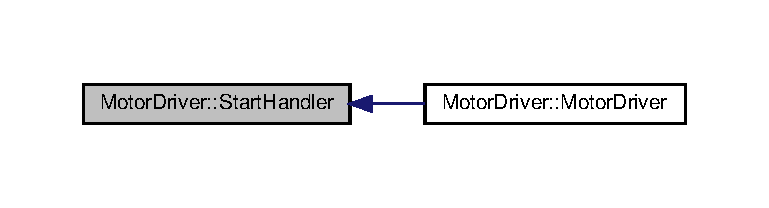
\includegraphics[width=350pt]{classMotorDriver_a64827491330490668bb8f8e57d0f3942_icgraph}
\end{center}
\end{figure}
\mbox{\Hypertarget{classMotorDriver_a5ebab90ca98fa04463de1cbae76af994}\label{classMotorDriver_a5ebab90ca98fa04463de1cbae76af994}} 
\index{Motor\+Driver@{Motor\+Driver}!Start\+Motor@{Start\+Motor}}
\index{Start\+Motor@{Start\+Motor}!Motor\+Driver@{Motor\+Driver}}
\subsubsection{\texorpdfstring{Start\+Motor()}{StartMotor()}}
{\footnotesize\ttfamily void Motor\+Driver\+::\+Start\+Motor (\begin{DoxyParamCaption}{ }\end{DoxyParamCaption})\hspace{0.3cm}{\ttfamily [private]}}



Responsible for starting the motor, i.\+e. setups the driver and sets required velocity of motor. 

Here is the call graph for this function\+:
\nopagebreak
\begin{figure}[H]
\begin{center}
\leavevmode
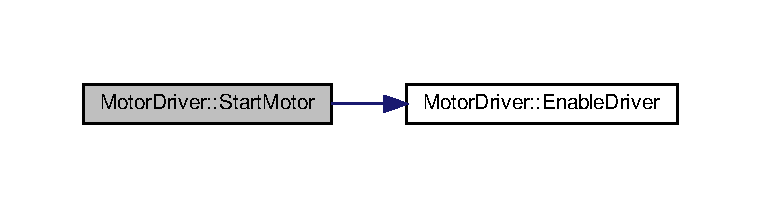
\includegraphics[width=350pt]{classMotorDriver_a5ebab90ca98fa04463de1cbae76af994_cgraph}
\end{center}
\end{figure}
Here is the caller graph for this function\+:
\nopagebreak
\begin{figure}[H]
\begin{center}
\leavevmode
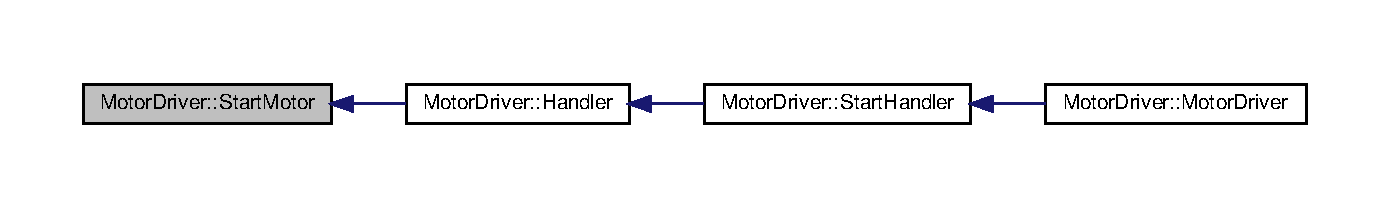
\includegraphics[width=350pt]{classMotorDriver_a5ebab90ca98fa04463de1cbae76af994_icgraph}
\end{center}
\end{figure}
\mbox{\Hypertarget{classMotorDriver_a43c47b4f550a3ee08e7da340e699ba76}\label{classMotorDriver_a43c47b4f550a3ee08e7da340e699ba76}} 
\index{Motor\+Driver@{Motor\+Driver}!Stop\+Handler@{Stop\+Handler}}
\index{Stop\+Handler@{Stop\+Handler}!Motor\+Driver@{Motor\+Driver}}
\subsubsection{\texorpdfstring{Stop\+Handler()}{StopHandler()}}
{\footnotesize\ttfamily void Motor\+Driver\+::\+Stop\+Handler (\begin{DoxyParamCaption}{ }\end{DoxyParamCaption})}



Stop handler thread. 

Here is the caller graph for this function\+:
\nopagebreak
\begin{figure}[H]
\begin{center}
\leavevmode
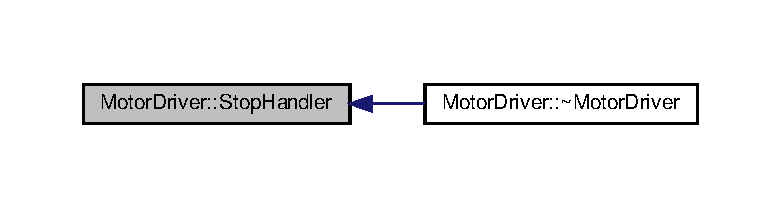
\includegraphics[width=350pt]{classMotorDriver_a43c47b4f550a3ee08e7da340e699ba76_icgraph}
\end{center}
\end{figure}
\mbox{\Hypertarget{classMotorDriver_aff8659e64841fb4b97c23b3494cd0575}\label{classMotorDriver_aff8659e64841fb4b97c23b3494cd0575}} 
\index{Motor\+Driver@{Motor\+Driver}!Stop\+Motor@{Stop\+Motor}}
\index{Stop\+Motor@{Stop\+Motor}!Motor\+Driver@{Motor\+Driver}}
\subsubsection{\texorpdfstring{Stop\+Motor()}{StopMotor()}}
{\footnotesize\ttfamily void Motor\+Driver\+::\+Stop\+Motor (\begin{DoxyParamCaption}{ }\end{DoxyParamCaption})\hspace{0.3cm}{\ttfamily [private]}}



Responsible for stopping the motor, i.\+e. disables the driver and sets velocity of motor to zero. 

Here is the call graph for this function\+:
\nopagebreak
\begin{figure}[H]
\begin{center}
\leavevmode
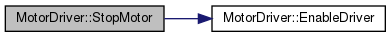
\includegraphics[width=350pt]{classMotorDriver_aff8659e64841fb4b97c23b3494cd0575_cgraph}
\end{center}
\end{figure}
Here is the caller graph for this function\+:
\nopagebreak
\begin{figure}[H]
\begin{center}
\leavevmode
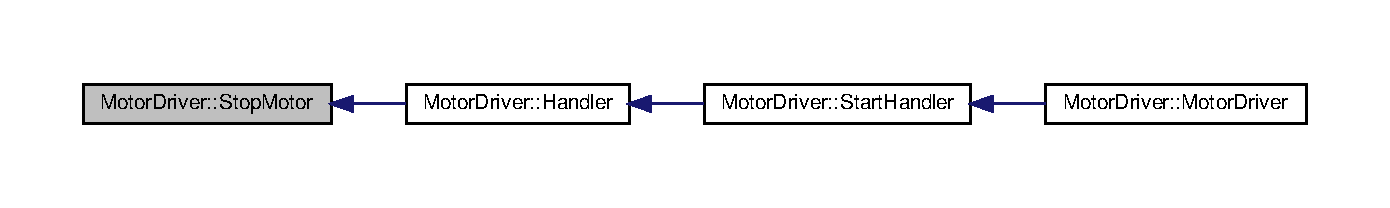
\includegraphics[width=350pt]{classMotorDriver_aff8659e64841fb4b97c23b3494cd0575_icgraph}
\end{center}
\end{figure}
\mbox{\Hypertarget{classMotorDriver_a04e97c6adc4df4d186d6799dfd8165b2}\label{classMotorDriver_a04e97c6adc4df4d186d6799dfd8165b2}} 
\index{Motor\+Driver@{Motor\+Driver}!Update\+Calib\+Params@{Update\+Calib\+Params}}
\index{Update\+Calib\+Params@{Update\+Calib\+Params}!Motor\+Driver@{Motor\+Driver}}
\subsubsection{\texorpdfstring{Update\+Calib\+Params()}{UpdateCalibParams()}}
{\footnotesize\ttfamily void Motor\+Driver\+::\+Update\+Calib\+Params (\begin{DoxyParamCaption}\item[{\hyperlink{structCONFIG__SET_1_1CALIB__PARAMS}{C\+O\+N\+F\+I\+G\+\_\+\+S\+E\+T\+::\+C\+A\+L\+I\+B\+\_\+\+P\+A\+R\+A\+MS}}]{calib\+\_\+param }\end{DoxyParamCaption})}



Updates calibration parameters to be used by motor driver. 

Here is the call graph for this function\+:
\nopagebreak
\begin{figure}[H]
\begin{center}
\leavevmode
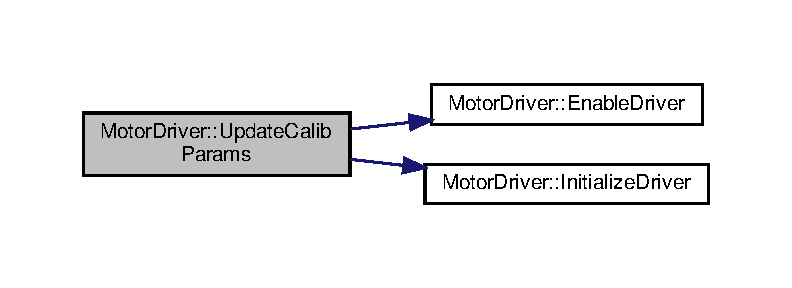
\includegraphics[width=350pt]{classMotorDriver_a04e97c6adc4df4d186d6799dfd8165b2_cgraph}
\end{center}
\end{figure}
Here is the caller graph for this function\+:
\nopagebreak
\begin{figure}[H]
\begin{center}
\leavevmode
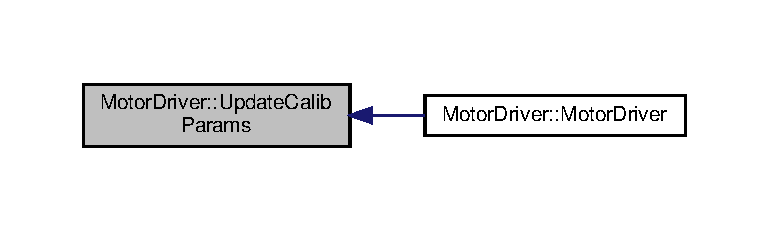
\includegraphics[width=350pt]{classMotorDriver_a04e97c6adc4df4d186d6799dfd8165b2_icgraph}
\end{center}
\end{figure}


\subsection{Member Data Documentation}
\mbox{\Hypertarget{classMotorDriver_acc772188969ac8c859d1e9c800eb0076}\label{classMotorDriver_acc772188969ac8c859d1e9c800eb0076}} 
\index{Motor\+Driver@{Motor\+Driver}!blind\+\_\+traversal\+\_\+requested\+\_\+@{blind\+\_\+traversal\+\_\+requested\+\_\+}}
\index{blind\+\_\+traversal\+\_\+requested\+\_\+@{blind\+\_\+traversal\+\_\+requested\+\_\+}!Motor\+Driver@{Motor\+Driver}}
\subsubsection{\texorpdfstring{blind\+\_\+traversal\+\_\+requested\+\_\+}{blind\_traversal\_requested\_}}
{\footnotesize\ttfamily bool Motor\+Driver\+::blind\+\_\+traversal\+\_\+requested\+\_\+ = false\hspace{0.3cm}{\ttfamily [private]}}

\mbox{\Hypertarget{classMotorDriver_aa2d3e952c7708106df0c86196490a499}\label{classMotorDriver_aa2d3e952c7708106df0c86196490a499}} 
\index{Motor\+Driver@{Motor\+Driver}!calib\+\_\+params\+\_\+@{calib\+\_\+params\+\_\+}}
\index{calib\+\_\+params\+\_\+@{calib\+\_\+params\+\_\+}!Motor\+Driver@{Motor\+Driver}}
\subsubsection{\texorpdfstring{calib\+\_\+params\+\_\+}{calib\_params\_}}
{\footnotesize\ttfamily \hyperlink{structCONFIG__SET_1_1CALIB__PARAMS}{C\+O\+N\+F\+I\+G\+\_\+\+S\+E\+T\+::\+C\+A\+L\+I\+B\+\_\+\+P\+A\+R\+A\+MS} Motor\+Driver\+::calib\+\_\+params\+\_\+\hspace{0.3cm}{\ttfamily [private]}}

\mbox{\Hypertarget{classMotorDriver_a9072fc26381b16a6a5e39ab1d7ed1e46}\label{classMotorDriver_a9072fc26381b16a6a5e39ab1d7ed1e46}} 
\index{Motor\+Driver@{Motor\+Driver}!current\+\_\+step\+\_\+@{current\+\_\+step\+\_\+}}
\index{current\+\_\+step\+\_\+@{current\+\_\+step\+\_\+}!Motor\+Driver@{Motor\+Driver}}
\subsubsection{\texorpdfstring{current\+\_\+step\+\_\+}{current\_step\_}}
{\footnotesize\ttfamily int Motor\+Driver\+::current\+\_\+step\+\_\+ = 0\hspace{0.3cm}{\ttfamily [static]}, {\ttfamily [private]}}

\mbox{\Hypertarget{classMotorDriver_a09cb1d904ff0b9ce54f17fa54aec8c70}\label{classMotorDriver_a09cb1d904ff0b9ce54f17fa54aec8c70}} 
\index{Motor\+Driver@{Motor\+Driver}!direction\+\_\+@{direction\+\_\+}}
\index{direction\+\_\+@{direction\+\_\+}!Motor\+Driver@{Motor\+Driver}}
\subsubsection{\texorpdfstring{direction\+\_\+}{direction\_}}
{\footnotesize\ttfamily bool Motor\+Driver\+::direction\+\_\+ = false\hspace{0.3cm}{\ttfamily [static]}, {\ttfamily [private]}}

\mbox{\Hypertarget{classMotorDriver_ad99c6f2f224f78428b137f7856cfba4b}\label{classMotorDriver_ad99c6f2f224f78428b137f7856cfba4b}} 
\index{Motor\+Driver@{Motor\+Driver}!driver\+\_\+status\+\_\+@{driver\+\_\+status\+\_\+}}
\index{driver\+\_\+status\+\_\+@{driver\+\_\+status\+\_\+}!Motor\+Driver@{Motor\+Driver}}
\subsubsection{\texorpdfstring{driver\+\_\+status\+\_\+}{driver\_status\_}}
{\footnotesize\ttfamily \hyperlink{namespaceCONFIG__SET_a722f4ba49e35faf1a2504aa23677b2f0}{C\+O\+N\+F\+I\+G\+\_\+\+S\+E\+T\+::\+D\+R\+I\+V\+E\+R\+\_\+\+S\+T\+A\+T\+US} Motor\+Driver\+::driver\+\_\+status\+\_\+\hspace{0.3cm}{\ttfamily [private]}}

\mbox{\Hypertarget{classMotorDriver_a140b9b922847586721725b7e76943c1e}\label{classMotorDriver_a140b9b922847586721725b7e76943c1e}} 
\index{Motor\+Driver@{Motor\+Driver}!expected\+\_\+step\+\_\+@{expected\+\_\+step\+\_\+}}
\index{expected\+\_\+step\+\_\+@{expected\+\_\+step\+\_\+}!Motor\+Driver@{Motor\+Driver}}
\subsubsection{\texorpdfstring{expected\+\_\+step\+\_\+}{expected\_step\_}}
{\footnotesize\ttfamily int Motor\+Driver\+::expected\+\_\+step\+\_\+ = 0\hspace{0.3cm}{\ttfamily [private]}}

\mbox{\Hypertarget{classMotorDriver_ab49b3ca9359af0016c206960887349b1}\label{classMotorDriver_ab49b3ca9359af0016c206960887349b1}} 
\index{Motor\+Driver@{Motor\+Driver}!full\+\_\+rot\+\_\+step\+\_\+count\+\_\+@{full\+\_\+rot\+\_\+step\+\_\+count\+\_\+}}
\index{full\+\_\+rot\+\_\+step\+\_\+count\+\_\+@{full\+\_\+rot\+\_\+step\+\_\+count\+\_\+}!Motor\+Driver@{Motor\+Driver}}
\subsubsection{\texorpdfstring{full\+\_\+rot\+\_\+step\+\_\+count\+\_\+}{full\_rot\_step\_count\_}}
{\footnotesize\ttfamily int Motor\+Driver\+::full\+\_\+rot\+\_\+step\+\_\+count\+\_\+ = (4 $\ast$ \hyperlink{namespaceCONFIG__SET_a7028034ed96d5ef10a87d1cdc12c5d27}{C\+O\+N\+F\+I\+G\+\_\+\+S\+E\+T\+::\+M\+O\+T\+O\+R\+\_\+\+D\+R\+I\+V\+E\+R\+\_\+\+M\+I\+C\+R\+O\+S\+T\+EP})\hspace{0.3cm}{\ttfamily [static]}, {\ttfamily [private]}}

\mbox{\Hypertarget{classMotorDriver_aec36906063e5e09d5bb7f7843f526874}\label{classMotorDriver_aec36906063e5e09d5bb7f7843f526874}} 
\index{Motor\+Driver@{Motor\+Driver}!handler\+\_\+thread\+\_\+@{handler\+\_\+thread\+\_\+}}
\index{handler\+\_\+thread\+\_\+@{handler\+\_\+thread\+\_\+}!Motor\+Driver@{Motor\+Driver}}
\subsubsection{\texorpdfstring{handler\+\_\+thread\+\_\+}{handler\_thread\_}}
{\footnotesize\ttfamily std\+::unique\+\_\+ptr$<$std\+::thread$>$ Motor\+Driver\+::handler\+\_\+thread\+\_\+ \{nullptr\}\hspace{0.3cm}{\ttfamily [private]}}

\mbox{\Hypertarget{classMotorDriver_abbc66ce217161de9ed45003718cd6c0e}\label{classMotorDriver_abbc66ce217161de9ed45003718cd6c0e}} 
\index{Motor\+Driver@{Motor\+Driver}!is\+\_\+motor\+\_\+running\+\_\+@{is\+\_\+motor\+\_\+running\+\_\+}}
\index{is\+\_\+motor\+\_\+running\+\_\+@{is\+\_\+motor\+\_\+running\+\_\+}!Motor\+Driver@{Motor\+Driver}}
\subsubsection{\texorpdfstring{is\+\_\+motor\+\_\+running\+\_\+}{is\_motor\_running\_}}
{\footnotesize\ttfamily bool Motor\+Driver\+::is\+\_\+motor\+\_\+running\+\_\+ = false\hspace{0.3cm}{\ttfamily [private]}}

\mbox{\Hypertarget{classMotorDriver_a930d873aa0a5961bd49b8b68553f5044}\label{classMotorDriver_a930d873aa0a5961bd49b8b68553f5044}} 
\index{Motor\+Driver@{Motor\+Driver}!keep\+\_\+handler\+\_\+running\+\_\+@{keep\+\_\+handler\+\_\+running\+\_\+}}
\index{keep\+\_\+handler\+\_\+running\+\_\+@{keep\+\_\+handler\+\_\+running\+\_\+}!Motor\+Driver@{Motor\+Driver}}
\subsubsection{\texorpdfstring{keep\+\_\+handler\+\_\+running\+\_\+}{keep\_handler\_running\_}}
{\footnotesize\ttfamily bool Motor\+Driver\+::keep\+\_\+handler\+\_\+running\+\_\+ = false\hspace{0.3cm}{\ttfamily [private]}}

\mbox{\Hypertarget{classMotorDriver_a938712bd2b784e0db660fdb30ad312af}\label{classMotorDriver_a938712bd2b784e0db660fdb30ad312af}} 
\index{Motor\+Driver@{Motor\+Driver}!last\+\_\+motor\+\_\+start\+\_\+time\+\_\+sec\+\_\+@{last\+\_\+motor\+\_\+start\+\_\+time\+\_\+sec\+\_\+}}
\index{last\+\_\+motor\+\_\+start\+\_\+time\+\_\+sec\+\_\+@{last\+\_\+motor\+\_\+start\+\_\+time\+\_\+sec\+\_\+}!Motor\+Driver@{Motor\+Driver}}
\subsubsection{\texorpdfstring{last\+\_\+motor\+\_\+start\+\_\+time\+\_\+sec\+\_\+}{last\_motor\_start\_time\_sec\_}}
{\footnotesize\ttfamily std\+::time\+\_\+t Motor\+Driver\+::last\+\_\+motor\+\_\+start\+\_\+time\+\_\+sec\+\_\+ = std\+::time(nullptr)\hspace{0.3cm}{\ttfamily [private]}}

\mbox{\Hypertarget{classMotorDriver_a6c443fae635cf2b50bfa205ac4f6418e}\label{classMotorDriver_a6c443fae635cf2b50bfa205ac4f6418e}} 
\index{Motor\+Driver@{Motor\+Driver}!logger\+\_\+@{logger\+\_\+}}
\index{logger\+\_\+@{logger\+\_\+}!Motor\+Driver@{Motor\+Driver}}
\subsubsection{\texorpdfstring{logger\+\_\+}{logger\_}}
{\footnotesize\ttfamily std\+::shared\+\_\+ptr$<$\hyperlink{classLogging}{Logging}$>$ Motor\+Driver\+::logger\+\_\+\hspace{0.3cm}{\ttfamily [private]}}

\mbox{\Hypertarget{classMotorDriver_a86d3f7015a61c62463ea3e718c5bba1c}\label{classMotorDriver_a86d3f7015a61c62463ea3e718c5bba1c}} 
\index{Motor\+Driver@{Motor\+Driver}!step\+\_\+timer\+\_\+@{step\+\_\+timer\+\_\+}}
\index{step\+\_\+timer\+\_\+@{step\+\_\+timer\+\_\+}!Motor\+Driver@{Motor\+Driver}}
\subsubsection{\texorpdfstring{step\+\_\+timer\+\_\+}{step\_timer\_}}
{\footnotesize\ttfamily hw\+\_\+timer\+\_\+t$\ast$ Motor\+Driver\+::step\+\_\+timer\+\_\+ = N\+U\+LL\hspace{0.3cm}{\ttfamily [private]}}

\mbox{\Hypertarget{classMotorDriver_a6c190777a6bcad1ea12f73707ed67de9}\label{classMotorDriver_a6c190777a6bcad1ea12f73707ed67de9}} 
\index{Motor\+Driver@{Motor\+Driver}!stop\+\_\+requested\+\_\+@{stop\+\_\+requested\+\_\+}}
\index{stop\+\_\+requested\+\_\+@{stop\+\_\+requested\+\_\+}!Motor\+Driver@{Motor\+Driver}}
\subsubsection{\texorpdfstring{stop\+\_\+requested\+\_\+}{stop\_requested\_}}
{\footnotesize\ttfamily bool Motor\+Driver\+::stop\+\_\+requested\+\_\+ = false\hspace{0.3cm}{\ttfamily [private]}}



The documentation for this class was generated from the following files\+:\begin{DoxyCompactItemize}
\item 
mvp/src/motor\+\_\+driver/\hyperlink{motor__driver_8h}{motor\+\_\+driver.\+h}\item 
mvp/src/motor\+\_\+driver/\hyperlink{motor__driver_8cpp}{motor\+\_\+driver.\+cpp}\end{DoxyCompactItemize}

\hypertarget{classStorage}{}\section{Storage Class Reference}
\label{classStorage}\index{Storage@{Storage}}
\subsection*{Public Member Functions}
\begin{DoxyCompactItemize}
\item 
\mbox{\Hypertarget{classStorage_a80ef6af5e4c9fd4424ae16e808d05291}\label{classStorage_a80ef6af5e4c9fd4424ae16e808d05291}} 
\hyperlink{classStorage_a80ef6af5e4c9fd4424ae16e808d05291}{Storage} ()
\begin{DoxyCompactList}\small\item\em Construct a new \hyperlink{classStorage}{Storage} object. \end{DoxyCompactList}\item 
\mbox{\Hypertarget{classStorage_a73cf30f0a34250396f9eabee7dc5c93d}\label{classStorage_a73cf30f0a34250396f9eabee7dc5c93d}} 
\hyperlink{classStorage_a73cf30f0a34250396f9eabee7dc5c93d}{$\sim$\+Storage} ()
\begin{DoxyCompactList}\small\item\em Destroy the \hyperlink{classStorage}{Storage} object. \end{DoxyCompactList}\item 
\mbox{\Hypertarget{classStorage_a0cdf803ccf0ea01b54103d2bf04c66d5}\label{classStorage_a0cdf803ccf0ea01b54103d2bf04c66d5}} 
void \hyperlink{classStorage_a0cdf803ccf0ea01b54103d2bf04c66d5}{test\+\_\+function} ()
\begin{DoxyCompactList}\small\item\em Hello. \end{DoxyCompactList}\end{DoxyCompactItemize}


The documentation for this class was generated from the following file\+:\begin{DoxyCompactItemize}
\item 
/home/mahi/git/automatic\+\_\+curtain/mvp/src/storage/\hyperlink{storage_8h}{storage.\+h}\end{DoxyCompactItemize}

\chapter{File Documentation}
\hypertarget{alexa__interaction_8cpp}{}\section{/home/mahi/git/automatic\+\_\+curtain/mvp/src/alexa\+\_\+interaction/alexa\+\_\+interaction.cpp File Reference}
\label{alexa__interaction_8cpp}\index{/home/mahi/git/automatic\+\_\+curtain/mvp/src/alexa\+\_\+interaction/alexa\+\_\+interaction.\+cpp@{/home/mahi/git/automatic\+\_\+curtain/mvp/src/alexa\+\_\+interaction/alexa\+\_\+interaction.\+cpp}}


Contains algorithms for handling alexa requests and make appropriate call at every request.  




\subsection{Detailed Description}
Contains algorithms for handling alexa requests and make appropriate call at every request. 

\begin{DoxyAuthor}{Author}
Dhiraj Deshmukh (\href{mailto:deshmukhdhiraj15@gmail.com}{\tt deshmukhdhiraj15@gmail.\+com}) 
\end{DoxyAuthor}
\begin{DoxyVersion}{Version}
0.\+1 
\end{DoxyVersion}
\begin{DoxyDate}{Date}
2022-\/07-\/20
\end{DoxyDate}
\begin{DoxyCopyright}{Copyright}
Copyright (c) 2022 
\end{DoxyCopyright}

\hypertarget{alexa__interaction_8h}{}\section{/home/mahi/git/automatic\+\_\+curtain/mvp/src/alexa\+\_\+interaction/alexa\+\_\+interaction.h File Reference}
\label{alexa__interaction_8h}\index{/home/mahi/git/automatic\+\_\+curtain/mvp/src/alexa\+\_\+interaction/alexa\+\_\+interaction.\+h@{/home/mahi/git/automatic\+\_\+curtain/mvp/src/alexa\+\_\+interaction/alexa\+\_\+interaction.\+h}}


Defines structure for class which will be interacting with alexa A\+PI.  


\subsection*{Classes}
\begin{DoxyCompactItemize}
\item 
class \hyperlink{classAlexaInteraction}{Alexa\+Interaction}
\end{DoxyCompactItemize}


\subsection{Detailed Description}
Defines structure for class which will be interacting with alexa A\+PI. 

\begin{DoxyAuthor}{Author}
Mahimana Bhatt (\href{mailto:mahimanabhatt@gmail.com}{\tt mahimanabhatt@gmail.\+com}) 
\end{DoxyAuthor}
\begin{DoxyVersion}{Version}
0.\+1 
\end{DoxyVersion}
\begin{DoxyDate}{Date}
2022-\/07-\/20
\end{DoxyDate}
\begin{DoxyCopyright}{Copyright}
Copyright (c) 2022 
\end{DoxyCopyright}

\hypertarget{config_8h}{}\section{mvp/src/config/config.h File Reference}
\label{config_8h}\index{mvp/src/config/config.\+h@{mvp/src/config/config.\+h}}


This header file contains all the constants and enum that will be used throughout the repository like specific pins, mapping from state to led color etc.  


{\ttfamily \#include $<$Arduino.\+h$>$}\newline
{\ttfamily \#include $<$chrono$>$}\newline
{\ttfamily \#include $<$cstdint$>$}\newline
{\ttfamily \#include $<$deque$>$}\newline
{\ttfamily \#include $<$iostream$>$}\newline
Include dependency graph for config.\+h\+:
\nopagebreak
\begin{figure}[H]
\begin{center}
\leavevmode
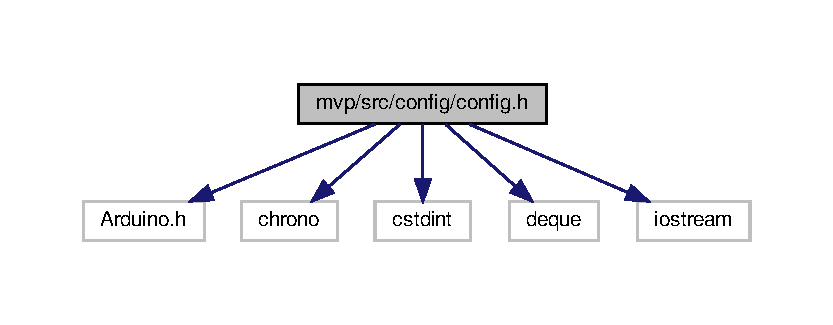
\includegraphics[width=350pt]{config_8h__incl}
\end{center}
\end{figure}
This graph shows which files directly or indirectly include this file\+:
\nopagebreak
\begin{figure}[H]
\begin{center}
\leavevmode
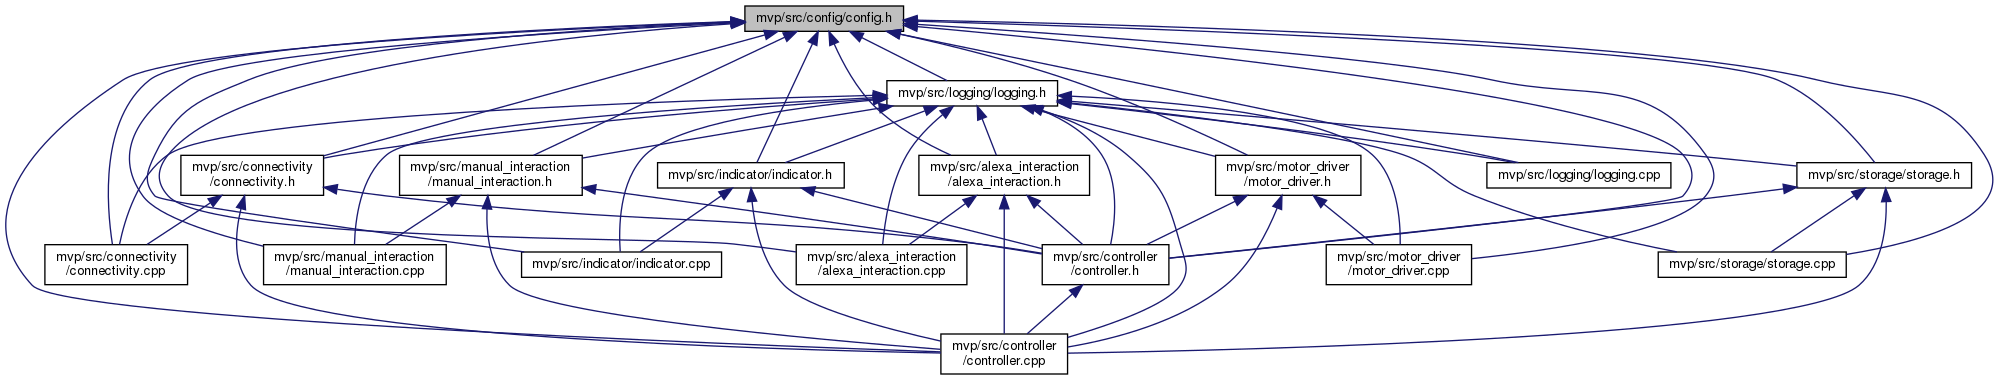
\includegraphics[width=350pt]{config_8h__dep__incl}
\end{center}
\end{figure}
\subsection*{Classes}
\begin{DoxyCompactItemize}
\item 
struct \hyperlink{structCONFIG__SET_1_1MOTION__REQUEST}{C\+O\+N\+F\+I\+G\+\_\+\+S\+E\+T\+::\+M\+O\+T\+I\+O\+N\+\_\+\+R\+E\+Q\+U\+E\+ST}
\item 
struct \hyperlink{structCONFIG__SET_1_1DEVICE__CRED}{C\+O\+N\+F\+I\+G\+\_\+\+S\+E\+T\+::\+D\+E\+V\+I\+C\+E\+\_\+\+C\+R\+ED}
\item 
struct \hyperlink{structCONFIG__SET_1_1CALIB__PARAMS}{C\+O\+N\+F\+I\+G\+\_\+\+S\+E\+T\+::\+C\+A\+L\+I\+B\+\_\+\+P\+A\+R\+A\+MS}
\end{DoxyCompactItemize}
\subsection*{Namespaces}
\begin{DoxyCompactItemize}
\item 
 \hyperlink{namespaceCONFIG__SET}{C\+O\+N\+F\+I\+G\+\_\+\+S\+ET}
\begin{DoxyCompactList}\small\item\em Namespace to be used for constants/enums. \end{DoxyCompactList}\end{DoxyCompactItemize}
\subsection*{Typedefs}
\begin{DoxyCompactItemize}
\item 
using \hyperlink{namespaceCONFIG__SET_a8816a22e7885d027a52bfa0d24fa9008}{C\+O\+N\+F\+I\+G\+\_\+\+S\+E\+T\+::time\+\_\+var} = std\+::chrono\+::time\+\_\+point$<$ std\+::chrono\+::system\+\_\+clock $>$
\item 
using \hyperlink{namespaceCONFIG__SET_a7a1c6f926aead4885c03f1fbeee693ce}{C\+O\+N\+F\+I\+G\+\_\+\+S\+E\+T\+::current\+\_\+time} = std\+::chrono\+::system\+\_\+clock
\end{DoxyCompactItemize}
\subsection*{Enumerations}
\begin{DoxyCompactItemize}
\item 
enum \hyperlink{namespaceCONFIG__SET_ac5c2592b79bead7e6497c37cddc401e6}{C\+O\+N\+F\+I\+G\+\_\+\+S\+E\+T\+::\+O\+P\+E\+R\+A\+T\+I\+O\+N\+\_\+\+M\+O\+DE} \{ \hyperlink{namespaceCONFIG__SET_ac5c2592b79bead7e6497c37cddc401e6ab5859d8721cfdc0312b2838b9c985bc1}{C\+O\+N\+F\+I\+G\+\_\+\+S\+E\+T\+::\+O\+P\+E\+R\+A\+T\+I\+O\+N\+\_\+\+M\+O\+D\+E\+::\+R\+E\+S\+ET}, 
\hyperlink{namespaceCONFIG__SET_ac5c2592b79bead7e6497c37cddc401e6aa49182544bf417d2e02cae1f35c9c8b8}{C\+O\+N\+F\+I\+G\+\_\+\+S\+E\+T\+::\+O\+P\+E\+R\+A\+T\+I\+O\+N\+\_\+\+M\+O\+D\+E\+::\+M\+A\+I\+N\+T\+E\+N\+A\+N\+CE}, 
\hyperlink{namespaceCONFIG__SET_ac5c2592b79bead7e6497c37cddc401e6a2e40ad879e955201df4dedbf8d479a12}{C\+O\+N\+F\+I\+G\+\_\+\+S\+E\+T\+::\+O\+P\+E\+R\+A\+T\+I\+O\+N\+\_\+\+M\+O\+D\+E\+::\+U\+S\+ER}, 
\hyperlink{namespaceCONFIG__SET_ac5c2592b79bead7e6497c37cddc401e6ad4cd0dabcf4caa22ad92fab40844c786}{C\+O\+N\+F\+I\+G\+\_\+\+S\+E\+T\+::\+O\+P\+E\+R\+A\+T\+I\+O\+N\+\_\+\+M\+O\+D\+E\+::\+NA}
 \}
\item 
enum \hyperlink{namespaceCONFIG__SET_aaf9764960ee214f0eaabd2461e30e932}{C\+O\+N\+F\+I\+G\+\_\+\+S\+E\+T\+::\+L\+O\+G\+\_\+\+T\+Y\+PE} \{ \hyperlink{namespaceCONFIG__SET_aaf9764960ee214f0eaabd2461e30e932a551b723eafd6a31d444fcb2f5920fbd3}{C\+O\+N\+F\+I\+G\+\_\+\+S\+E\+T\+::\+L\+O\+G\+\_\+\+T\+Y\+P\+E\+::\+I\+N\+FO}, 
\hyperlink{namespaceCONFIG__SET_aaf9764960ee214f0eaabd2461e30e932abb1ca97ec761fc37101737ba0aa2e7c5}{C\+O\+N\+F\+I\+G\+\_\+\+S\+E\+T\+::\+L\+O\+G\+\_\+\+T\+Y\+P\+E\+::\+E\+R\+R\+OR}, 
\hyperlink{namespaceCONFIG__SET_aaf9764960ee214f0eaabd2461e30e932a32bd8a1db2275458673903bdb84cb277}{C\+O\+N\+F\+I\+G\+\_\+\+S\+E\+T\+::\+L\+O\+G\+\_\+\+T\+Y\+P\+E\+::\+W\+A\+RN}
 \}
\item 
enum \hyperlink{namespaceCONFIG__SET_a3c4daebec2ea4e9f6affb5b3abbeb863}{C\+O\+N\+F\+I\+G\+\_\+\+S\+E\+T\+::\+L\+O\+G\+\_\+\+C\+L\+A\+SS} \{ \newline
\hyperlink{namespaceCONFIG__SET_a3c4daebec2ea4e9f6affb5b3abbeb863a42e074e8564dad9034ef033c6a6cf8b6}{C\+O\+N\+F\+I\+G\+\_\+\+S\+E\+T\+::\+L\+O\+G\+\_\+\+C\+L\+A\+S\+S\+::\+C\+O\+N\+T\+R\+O\+L\+L\+ER}, 
\hyperlink{namespaceCONFIG__SET_a3c4daebec2ea4e9f6affb5b3abbeb863afe45874d234b693c3648a37d604b0865}{C\+O\+N\+F\+I\+G\+\_\+\+S\+E\+T\+::\+L\+O\+G\+\_\+\+C\+L\+A\+S\+S\+::\+C\+O\+N\+N\+E\+C\+T\+I\+V\+I\+TY}, 
\hyperlink{namespaceCONFIG__SET_a3c4daebec2ea4e9f6affb5b3abbeb863a2b254b1e77ef0d4fe30639ee576bf05d}{C\+O\+N\+F\+I\+G\+\_\+\+S\+E\+T\+::\+L\+O\+G\+\_\+\+C\+L\+A\+S\+S\+::\+I\+N\+D\+I\+C\+A\+T\+OR}, 
\hyperlink{namespaceCONFIG__SET_a3c4daebec2ea4e9f6affb5b3abbeb863a042bca9f4ffd4cb8530fa2a9035e00c3}{C\+O\+N\+F\+I\+G\+\_\+\+S\+E\+T\+::\+L\+O\+G\+\_\+\+C\+L\+A\+S\+S\+::\+L\+O\+G\+G\+I\+NG}, 
\newline
\hyperlink{namespaceCONFIG__SET_a3c4daebec2ea4e9f6affb5b3abbeb863a0b83d32b63ae6ca0805d471c407c39a8}{C\+O\+N\+F\+I\+G\+\_\+\+S\+E\+T\+::\+L\+O\+G\+\_\+\+C\+L\+A\+S\+S\+::\+M\+A\+N\+U\+A\+L\+\_\+\+I\+N\+T\+E\+R\+A\+C\+T\+I\+ON}, 
\hyperlink{namespaceCONFIG__SET_a3c4daebec2ea4e9f6affb5b3abbeb863aef2f278882c5090b495fea73f0f14150}{C\+O\+N\+F\+I\+G\+\_\+\+S\+E\+T\+::\+L\+O\+G\+\_\+\+C\+L\+A\+S\+S\+::\+M\+O\+T\+O\+R\+\_\+\+D\+R\+I\+V\+ER}, 
\hyperlink{namespaceCONFIG__SET_a3c4daebec2ea4e9f6affb5b3abbeb863a754a5d433173b5ddc7debc2110ac575f}{C\+O\+N\+F\+I\+G\+\_\+\+S\+E\+T\+::\+L\+O\+G\+\_\+\+C\+L\+A\+S\+S\+::\+S\+T\+O\+R\+A\+GE}, 
\hyperlink{namespaceCONFIG__SET_a3c4daebec2ea4e9f6affb5b3abbeb863ad42bdb2009ad11a7ac3dd12ca97e81da}{C\+O\+N\+F\+I\+G\+\_\+\+S\+E\+T\+::\+L\+O\+G\+\_\+\+C\+L\+A\+S\+S\+::\+A\+L\+E\+X\+A\+\_\+\+I\+N\+T\+E\+R\+A\+C\+T\+I\+ON}
 \}
\item 
enum \hyperlink{namespaceCONFIG__SET_a627706be626fd4e58c539ed120c27748}{C\+O\+N\+F\+I\+G\+\_\+\+S\+E\+T\+::\+M\+A\+N\+U\+A\+L\+\_\+\+P\+U\+SH} \{ \newline
\hyperlink{namespaceCONFIG__SET_a627706be626fd4e58c539ed120c27748a201be4da83bb4099ea70c0fa017f69d5}{C\+O\+N\+F\+I\+G\+\_\+\+S\+E\+T\+::\+M\+A\+N\+U\+A\+L\+\_\+\+P\+U\+S\+H\+::\+N\+O\+\_\+\+P\+U\+SH}, 
\hyperlink{namespaceCONFIG__SET_a627706be626fd4e58c539ed120c27748a452fd0059d3faa302e1e7b98eb0b1e81}{C\+O\+N\+F\+I\+G\+\_\+\+S\+E\+T\+::\+M\+A\+N\+U\+A\+L\+\_\+\+P\+U\+S\+H\+::\+L\+O\+N\+G\+\_\+\+P\+R\+E\+S\+S\+\_\+\+UP}, 
\hyperlink{namespaceCONFIG__SET_a627706be626fd4e58c539ed120c27748aab27af1260dbe253aac03e395b9b23ff}{C\+O\+N\+F\+I\+G\+\_\+\+S\+E\+T\+::\+M\+A\+N\+U\+A\+L\+\_\+\+P\+U\+S\+H\+::\+L\+O\+N\+G\+\_\+\+P\+R\+E\+S\+S\+\_\+\+D\+O\+WN}, 
\hyperlink{namespaceCONFIG__SET_a627706be626fd4e58c539ed120c27748a88803b906ab3fb49d793794cccc85713}{C\+O\+N\+F\+I\+G\+\_\+\+S\+E\+T\+::\+M\+A\+N\+U\+A\+L\+\_\+\+P\+U\+S\+H\+::\+L\+O\+N\+G\+\_\+\+P\+R\+E\+S\+S\+\_\+\+B\+O\+TH}, 
\newline
\hyperlink{namespaceCONFIG__SET_a627706be626fd4e58c539ed120c27748ab985c91c3413dee3833c52f7587927d4}{C\+O\+N\+F\+I\+G\+\_\+\+S\+E\+T\+::\+M\+A\+N\+U\+A\+L\+\_\+\+P\+U\+S\+H\+::\+D\+O\+U\+B\+L\+E\+\_\+\+T\+A\+P\+\_\+\+UP}, 
\hyperlink{namespaceCONFIG__SET_a627706be626fd4e58c539ed120c27748a344b76ee59e91ead4475cd148aba681f}{C\+O\+N\+F\+I\+G\+\_\+\+S\+E\+T\+::\+M\+A\+N\+U\+A\+L\+\_\+\+P\+U\+S\+H\+::\+D\+O\+U\+B\+L\+E\+\_\+\+T\+A\+P\+\_\+\+D\+O\+WN}, 
\hyperlink{namespaceCONFIG__SET_a627706be626fd4e58c539ed120c27748ab6e371bad37f26516750c7661c68f491}{C\+O\+N\+F\+I\+G\+\_\+\+S\+E\+T\+::\+M\+A\+N\+U\+A\+L\+\_\+\+P\+U\+S\+H\+::\+D\+O\+U\+B\+L\+E\+\_\+\+T\+A\+P\+\_\+\+B\+O\+TH}
 \}
\item 
enum \hyperlink{namespaceCONFIG__SET_a94751f576b4a29d791e7871295c48b72}{C\+O\+N\+F\+I\+G\+\_\+\+S\+E\+T\+::\+B\+U\+T\+T\+O\+N\+\_\+\+P\+R\+E\+SS} \{ \hyperlink{namespaceCONFIG__SET_a94751f576b4a29d791e7871295c48b72a201be4da83bb4099ea70c0fa017f69d5}{C\+O\+N\+F\+I\+G\+\_\+\+S\+E\+T\+::\+B\+U\+T\+T\+O\+N\+\_\+\+P\+R\+E\+S\+S\+::\+N\+O\+\_\+\+P\+U\+SH}, 
\hyperlink{namespaceCONFIG__SET_a94751f576b4a29d791e7871295c48b72a6cfd612b64bbe4bd62ea3eacec312f2a}{C\+O\+N\+F\+I\+G\+\_\+\+S\+E\+T\+::\+B\+U\+T\+T\+O\+N\+\_\+\+P\+R\+E\+S\+S\+::\+L\+O\+N\+G\+\_\+\+P\+R\+E\+SS}, 
\hyperlink{namespaceCONFIG__SET_a94751f576b4a29d791e7871295c48b72a69262b7d2d5f239bbdeff40c30d17662}{C\+O\+N\+F\+I\+G\+\_\+\+S\+E\+T\+::\+B\+U\+T\+T\+O\+N\+\_\+\+P\+R\+E\+S\+S\+::\+D\+O\+U\+B\+L\+E\+\_\+\+T\+AP}
 \}
\item 
enum \hyperlink{namespaceCONFIG__SET_a8379cbe9f81ee38829b156f47261081a}{C\+O\+N\+F\+I\+G\+\_\+\+S\+E\+T\+::\+D\+E\+V\+I\+C\+E\+\_\+\+S\+T\+A\+T\+US} \{ \hyperlink{namespaceCONFIG__SET_a8379cbe9f81ee38829b156f47261081aa893b3aaf1661e3717b18e8335ff93a72}{C\+O\+N\+F\+I\+G\+\_\+\+S\+E\+T\+::\+D\+E\+V\+I\+C\+E\+\_\+\+S\+T\+A\+T\+U\+S\+::\+F\+A\+U\+LT}, 
\hyperlink{namespaceCONFIG__SET_a8379cbe9f81ee38829b156f47261081aa3fe019c6817599387124ce924e33c70b}{C\+O\+N\+F\+I\+G\+\_\+\+S\+E\+T\+::\+D\+E\+V\+I\+C\+E\+\_\+\+S\+T\+A\+T\+U\+S\+::\+O\+P\+E\+R\+A\+T\+I\+O\+N\+\_\+\+M\+O\+DE}, 
\hyperlink{namespaceCONFIG__SET_a8379cbe9f81ee38829b156f47261081aaba12d2493fc3be7067212035e03a7c04}{C\+O\+N\+F\+I\+G\+\_\+\+S\+E\+T\+::\+D\+E\+V\+I\+C\+E\+\_\+\+S\+T\+A\+T\+U\+S\+::\+R\+E\+S\+E\+T\+\_\+\+M\+O\+DE}, 
\hyperlink{namespaceCONFIG__SET_a8379cbe9f81ee38829b156f47261081aaaf0bd6c96a36aa63de9f0ac59060deea}{C\+O\+N\+F\+I\+G\+\_\+\+S\+E\+T\+::\+D\+E\+V\+I\+C\+E\+\_\+\+S\+T\+A\+T\+U\+S\+::\+M\+A\+I\+N\+T\+E\+N\+A\+N\+C\+E\+\_\+\+M\+O\+DE}
 \}
\item 
enum \hyperlink{namespaceCONFIG__SET_a722f4ba49e35faf1a2504aa23677b2f0}{C\+O\+N\+F\+I\+G\+\_\+\+S\+E\+T\+::\+D\+R\+I\+V\+E\+R\+\_\+\+S\+T\+A\+T\+US} \{ \hyperlink{namespaceCONFIG__SET_a722f4ba49e35faf1a2504aa23677b2f0a1588118736b5ecdb1ac20c16428d8ea7}{C\+O\+N\+F\+I\+G\+\_\+\+S\+E\+T\+::\+D\+R\+I\+V\+E\+R\+\_\+\+S\+T\+A\+T\+U\+S\+::\+A\+V\+A\+I\+L\+A\+B\+LE}, 
\hyperlink{namespaceCONFIG__SET_a722f4ba49e35faf1a2504aa23677b2f0a802706a9238e2928077f97736854bad4}{C\+O\+N\+F\+I\+G\+\_\+\+S\+E\+T\+::\+D\+R\+I\+V\+E\+R\+\_\+\+S\+T\+A\+T\+U\+S\+::\+B\+U\+SY}, 
\hyperlink{namespaceCONFIG__SET_a722f4ba49e35faf1a2504aa23677b2f0a81ec94fc396b06d900dfec53805d1732}{C\+O\+N\+F\+I\+G\+\_\+\+S\+E\+T\+::\+D\+R\+I\+V\+E\+R\+\_\+\+S\+T\+A\+T\+U\+S\+::\+I\+N\+\_\+\+A\+C\+T\+I\+VE}
 \}
\end{DoxyCompactItemize}
\subsection*{Variables}
\begin{DoxyCompactItemize}
\item 
const int \hyperlink{namespaceCONFIG__SET_aa9d9cee85d0c1416ccb5ed5f801de6db}{C\+O\+N\+F\+I\+G\+\_\+\+S\+E\+T\+::\+L\+O\+G\+G\+I\+N\+G\+\_\+\+B\+A\+U\+D\+\_\+\+R\+A\+TE} = 115200
\item 
const int \hyperlink{namespaceCONFIG__SET_a7db23e13f6ec09a9be65fad30733470e}{C\+O\+N\+F\+I\+G\+\_\+\+S\+E\+T\+::\+M\+O\+T\+O\+R\+\_\+\+D\+R\+I\+V\+E\+R\+\_\+\+B\+A\+U\+D\+\_\+\+R\+A\+TE} = 115200
\item 
const int \hyperlink{namespaceCONFIG__SET_a0d526cb827f2f3c5236874a4157448af}{C\+O\+N\+F\+I\+G\+\_\+\+S\+E\+T\+::\+T\+R\+Y\+\_\+\+R\+E\+C\+O\+N\+N\+E\+CT} = 3
\item 
const int \hyperlink{namespaceCONFIG__SET_a4a1488bbde32db8f3d362761adc7c637}{C\+O\+N\+F\+I\+G\+\_\+\+S\+E\+T\+::\+M\+A\+X\+\_\+\+S\+E\+C\+O\+N\+D\+S\+\_\+\+L\+O\+S\+T\+\_\+\+W\+I\+FI} = 600
\item 
const std\+::string \hyperlink{namespaceCONFIG__SET_adc424e5a5b81f2016a88456fd2f383d9}{C\+O\+N\+F\+I\+G\+\_\+\+S\+E\+T\+::\+S\+T\+O\+R\+A\+G\+E\+\_\+\+N\+A\+M\+E\+S\+P\+A\+CE} = \char`\"{}madac\char`\"{}
\item 
const int \hyperlink{namespaceCONFIG__SET_a91d987372150d727ecbb41b39d482911}{C\+O\+N\+F\+I\+G\+\_\+\+S\+E\+T\+::\+N\+U\+M\+B\+E\+R\+\_\+\+O\+F\+\_\+\+L\+E\+DS} = 1
\item 
const int \hyperlink{namespaceCONFIG__SET_ae380133af7dbc440e94dd1d32ca8011c}{C\+O\+N\+F\+I\+G\+\_\+\+S\+E\+T\+::\+L\+E\+D\+\_\+\+B\+R\+I\+G\+H\+T\+N\+E\+SS} = 25
\item 
const int \hyperlink{namespaceCONFIG__SET_af30cde25aaad1a3f7c1056df78fe44ef}{C\+O\+N\+F\+I\+G\+\_\+\+S\+E\+T\+::\+D\+E\+Q\+U\+E\+\_\+\+A\+N\+A\+L\+Y\+Z\+E\+R\+\_\+\+F\+R\+EQ} = 2
\item 
const std\+::string \hyperlink{namespaceCONFIG__SET_adc315222607c5e3c4aa1e0d13b6987ee}{C\+O\+N\+F\+I\+G\+\_\+\+S\+E\+T\+::\+K\+E\+Y\+\_\+\+S\+S\+ID} = \char`\"{}ssid\char`\"{}
\item 
const std\+::string \hyperlink{namespaceCONFIG__SET_a19f24640ed129493b066d05e146deaf3}{C\+O\+N\+F\+I\+G\+\_\+\+S\+E\+T\+::\+K\+E\+Y\+\_\+\+P\+A\+S\+S\+W\+O\+RD} = \char`\"{}password\char`\"{}
\item 
const std\+::string \hyperlink{namespaceCONFIG__SET_af0e474e6061134d6cbf04e0c890552d9}{C\+O\+N\+F\+I\+G\+\_\+\+S\+E\+T\+::\+K\+E\+Y\+\_\+\+D\+E\+V\+I\+C\+E\+\_\+\+ID} = \char`\"{}device\+ID\char`\"{}
\item 
const std\+::string \hyperlink{namespaceCONFIG__SET_acb991fe6c1317a4bf770b8b1a049ad25}{C\+O\+N\+F\+I\+G\+\_\+\+S\+E\+T\+::\+K\+E\+Y\+\_\+\+T\+O\+T\+A\+L\+\_\+\+S\+T\+E\+P\+\_\+\+C\+O\+U\+NT} = \char`\"{}total\+Step\+Count\char`\"{}
\item 
const std\+::string \hyperlink{namespaceCONFIG__SET_a01f506112394a3ac18b3a731a710984c}{C\+O\+N\+F\+I\+G\+\_\+\+S\+E\+T\+::\+K\+E\+Y\+\_\+\+D\+I\+R\+E\+C\+T\+I\+ON} = \char`\"{}direction\char`\"{}
\item 
const std\+::string \hyperlink{namespaceCONFIG__SET_a77febd18d2a2712e1357b057a52e9be3}{C\+O\+N\+F\+I\+G\+\_\+\+S\+E\+T\+::\+K\+E\+Y\+\_\+\+M\+O\+DE} = \char`\"{}mode\char`\"{}
\item 
const String \hyperlink{namespaceCONFIG__SET_a2ac88bd64607d4819d1bda478f469817}{C\+O\+N\+F\+I\+G\+\_\+\+S\+E\+T\+::\+D\+E\+F\+A\+U\+L\+T\+\_\+\+D\+E\+V\+I\+C\+E\+\_\+\+ID} = \char`\"{}madac\+\_\+blinds\char`\"{}
\item 
const float \hyperlink{namespaceCONFIG__SET_a8f23ef59b087dff79c434bd84525a915}{C\+O\+N\+F\+I\+G\+\_\+\+S\+E\+T\+::\+M\+O\+T\+O\+R\+\_\+\+D\+R\+I\+V\+E\+R\+\_\+\+R\+\_\+\+S\+E\+N\+SE} = 0.\+11f
\item 
const uint8\+\_\+t \hyperlink{namespaceCONFIG__SET_a6a76f57577e628d797a633669d8adced}{C\+O\+N\+F\+I\+G\+\_\+\+S\+E\+T\+::\+M\+O\+T\+O\+R\+\_\+\+D\+R\+I\+V\+E\+R\+\_\+\+A\+D\+D\+R\+E\+SS} = 0b00
\item 
const uint8\+\_\+t \hyperlink{namespaceCONFIG__SET_a9cd2f24701a5f7debb61387d734af3f7}{C\+O\+N\+F\+I\+G\+\_\+\+S\+E\+T\+::\+M\+O\+T\+O\+R\+\_\+\+D\+R\+I\+V\+E\+R\+\_\+\+T\+O\+FF} = 4
\item 
const uint8\+\_\+t \hyperlink{namespaceCONFIG__SET_abd06bbb93246b7d98d1e7c2e5e4954b4}{C\+O\+N\+F\+I\+G\+\_\+\+S\+E\+T\+::\+M\+O\+T\+O\+R\+\_\+\+D\+R\+I\+V\+E\+R\+\_\+\+B\+L\+A\+N\+K\+\_\+\+T\+I\+ME} = 24
\item 
const uint16\+\_\+t \hyperlink{namespaceCONFIG__SET_a367788b61bc20c95602dec7063093fce}{C\+O\+N\+F\+I\+G\+\_\+\+S\+E\+T\+::\+M\+O\+T\+O\+R\+\_\+\+D\+R\+I\+V\+E\+R\+\_\+\+R\+M\+S\+\_\+\+C\+U\+R\+R\+E\+NT} = 2000
\item 
const uint16\+\_\+t \hyperlink{namespaceCONFIG__SET_a7028034ed96d5ef10a87d1cdc12c5d27}{C\+O\+N\+F\+I\+G\+\_\+\+S\+E\+T\+::\+M\+O\+T\+O\+R\+\_\+\+D\+R\+I\+V\+E\+R\+\_\+\+M\+I\+C\+R\+O\+S\+T\+EP} = 16
\item 
const uint32\+\_\+t \hyperlink{namespaceCONFIG__SET_aaaf7add03a2bd7b4a1cad95838dc6545}{C\+O\+N\+F\+I\+G\+\_\+\+S\+E\+T\+::\+M\+O\+T\+O\+R\+\_\+\+D\+R\+I\+V\+E\+R\+\_\+\+T\+C\+O\+O\+L\+\_\+\+T\+H\+RS} = 0x\+F\+F\+F\+FF
\item 
const uint8\+\_\+t \hyperlink{namespaceCONFIG__SET_a32dc4d5c8cc5890bf7f9be0a7f15bdb2}{C\+O\+N\+F\+I\+G\+\_\+\+S\+E\+T\+::\+M\+O\+T\+O\+R\+\_\+\+D\+R\+I\+V\+E\+R\+\_\+\+S\+E\+\_\+\+M\+IN} = 0
\item 
const uint8\+\_\+t \hyperlink{namespaceCONFIG__SET_a790b63a59051c9e242aff5b4123a9ca5}{C\+O\+N\+F\+I\+G\+\_\+\+S\+E\+T\+::\+M\+O\+T\+O\+R\+\_\+\+D\+R\+I\+V\+E\+R\+\_\+\+S\+E\+\_\+\+M\+AX} = 2
\item 
const uint8\+\_\+t \hyperlink{namespaceCONFIG__SET_a957a048d0f02b3bca4145248c6d79c77}{C\+O\+N\+F\+I\+G\+\_\+\+S\+E\+T\+::\+M\+O\+T\+O\+R\+\_\+\+D\+R\+I\+V\+E\+R\+\_\+\+S\+E\+DN} = 0b01
\item 
const uint32\+\_\+t \hyperlink{namespaceCONFIG__SET_ad8683609012e266d026138915afb2c4c}{C\+O\+N\+F\+I\+G\+\_\+\+S\+E\+T\+::\+M\+O\+T\+O\+R\+\_\+\+D\+R\+I\+V\+E\+R\+\_\+\+M\+A\+X\+\_\+\+S\+P\+E\+ED} = 5000
\item 
const int \hyperlink{namespaceCONFIG__SET_a56ca50a3b66685f81410683733371590}{C\+O\+N\+F\+I\+G\+\_\+\+S\+E\+T\+::\+M\+O\+T\+O\+R\+\_\+\+D\+R\+I\+V\+E\+R\+\_\+\+S\+G\+\_\+\+T\+H\+R\+E\+SH} = 45
\item 
const int \hyperlink{namespaceCONFIG__SET_a4cfa726833e14a8607e9c4c8b5895792}{C\+O\+N\+F\+I\+G\+\_\+\+S\+E\+T\+::\+M\+O\+T\+O\+R\+\_\+\+S\+T\+O\+P\+\_\+\+T\+I\+M\+E\+\_\+\+S\+EC} = 120
\item 
const float \hyperlink{namespaceCONFIG__SET_ae98d33bba82717c83e577914428d2f87}{C\+O\+N\+F\+I\+G\+\_\+\+S\+E\+T\+::\+S\+T\+E\+P\+\_\+\+F\+R\+A\+C\+T\+I\+O\+N\+\_\+\+A\+L\+L\+O\+W\+A\+N\+CE} = 0.\+05
\item 
const int \hyperlink{namespaceCONFIG__SET_a4e51168ed48d5e6ff6bdd26da8fd0244}{C\+O\+N\+F\+I\+G\+\_\+\+S\+E\+T\+::\+M\+O\+D\+E\+\_\+\+E\+X\+P\+I\+R\+E\+\_\+\+T\+I\+M\+E\+\_\+\+L\+I\+M\+IT} = 300
\item 
const int \hyperlink{namespaceCONFIG__SET_a538190e043ad035b08b9fc653d6a0491}{C\+O\+N\+F\+I\+G\+\_\+\+S\+E\+T\+::\+W\+I\+F\+I\+\_\+\+D\+I\+S\+C\+O\+N\+N\+E\+C\+T\+\_\+\+R\+E\+S\+T\+A\+R\+T\+\_\+\+T\+I\+M\+E\+\_\+\+L\+I\+M\+IT} = 60
\item 
const int \hyperlink{namespaceCONFIG__SET_a932d38d647f5793b7ebb07de5c7baf7b}{C\+O\+N\+F\+I\+G\+\_\+\+S\+E\+T\+::\+P\+I\+N\+\_\+\+R\+G\+B\+\_\+\+L\+ED} = 32
\item 
static const int \hyperlink{namespaceCONFIG__SET_a2a69cb92b89581f4a67d29a1a808327b}{C\+O\+N\+F\+I\+G\+\_\+\+S\+E\+T\+::\+P\+I\+N\+\_\+\+B\+U\+T\+T\+O\+N\+\_\+\+UP} = 33
\item 
static const int \hyperlink{namespaceCONFIG__SET_a5bf40b051395303a194e7afab2a66d43}{C\+O\+N\+F\+I\+G\+\_\+\+S\+E\+T\+::\+P\+I\+N\+\_\+\+B\+U\+T\+T\+O\+N\+\_\+\+D\+O\+WN} = 25
\item 
const int \hyperlink{namespaceCONFIG__SET_a76e1dbd32a24123a8e1c6f1032553e9e}{C\+O\+N\+F\+I\+G\+\_\+\+S\+E\+T\+::\+P\+I\+N\+\_\+\+M\+D\+\_\+\+E\+N\+A\+B\+LE} = 4
\item 
const int \hyperlink{namespaceCONFIG__SET_a3cd5a807c53edf90423ef292df549a2c}{C\+O\+N\+F\+I\+G\+\_\+\+S\+E\+T\+::\+P\+I\+N\+\_\+\+M\+D\+\_\+\+RX} = 16
\item 
const int \hyperlink{namespaceCONFIG__SET_ae14a96410643d22f30b5e7f98bbc2e98}{C\+O\+N\+F\+I\+G\+\_\+\+S\+E\+T\+::\+P\+I\+N\+\_\+\+M\+D\+\_\+\+TX} = 17
\item 
const int \hyperlink{namespaceCONFIG__SET_af93fc82a783571bf68af757e1a59be8d}{C\+O\+N\+F\+I\+G\+\_\+\+S\+E\+T\+::\+P\+I\+N\+\_\+\+M\+D\+\_\+\+M\+S1} = 5
\item 
const int \hyperlink{namespaceCONFIG__SET_a3ae1a9238a4c2ef99018a568fb407188}{C\+O\+N\+F\+I\+G\+\_\+\+S\+E\+T\+::\+P\+I\+N\+\_\+\+M\+D\+\_\+\+M\+S2} = 18
\item 
const int \hyperlink{namespaceCONFIG__SET_a6ff1241febf3c05949aa4e9615126aaa}{C\+O\+N\+F\+I\+G\+\_\+\+S\+E\+T\+::\+P\+I\+N\+\_\+\+M\+D\+\_\+\+S\+T\+EP} = 22
\item 
const int \hyperlink{namespaceCONFIG__SET_a893c9a17e861d557ec6e6d009d02f1fd}{C\+O\+N\+F\+I\+G\+\_\+\+S\+E\+T\+::\+P\+I\+N\+\_\+\+M\+D\+\_\+\+D\+IR} = 23
\item 
const int \hyperlink{namespaceCONFIG__SET_a77c4124103e0be77050f54fed8f46cbe}{C\+O\+N\+F\+I\+G\+\_\+\+S\+E\+T\+::\+P\+I\+N\+\_\+\+M\+D\+\_\+\+I\+N\+D\+EX} = 21
\item 
const int \hyperlink{namespaceCONFIG__SET_a24d0005db5d888efec3ad54d1d21d319}{C\+O\+N\+F\+I\+G\+\_\+\+S\+E\+T\+::\+P\+I\+N\+\_\+\+M\+D\+\_\+\+D\+I\+AG} = 19
\end{DoxyCompactItemize}


\subsection{Detailed Description}
This header file contains all the constants and enum that will be used throughout the repository like specific pins, mapping from state to led color etc. 

\begin{DoxyAuthor}{Author}
Mahimana Bhatt (\href{mailto:mahimanabhatt@gmail.com}{\tt mahimanabhatt@gmail.\+com}) 
\end{DoxyAuthor}
\begin{DoxyVersion}{Version}
0.\+1 
\end{DoxyVersion}
\begin{DoxyDate}{Date}
2022-\/07-\/19
\end{DoxyDate}
\begin{DoxyCopyright}{Copyright}
Copyright (c) 2022 
\end{DoxyCopyright}

\hypertarget{connectivity_8cpp}{}\section{/home/mahi/git/automatic\+\_\+curtain/mvp/src/connectivity/connectivity.cpp File Reference}
\label{connectivity_8cpp}\index{/home/mahi/git/automatic\+\_\+curtain/mvp/src/connectivity/connectivity.\+cpp@{/home/mahi/git/automatic\+\_\+curtain/mvp/src/connectivity/connectivity.\+cpp}}


Contains algorithms related to connecting to Wi\+Fi, O\+TA updates and webpage display.  




\subsection{Detailed Description}
Contains algorithms related to connecting to Wi\+Fi, O\+TA updates and webpage display. 

\begin{DoxyAuthor}{Author}
Dhiraj Deshmukh (\href{mailto:deshmukhdhiraj15@gmail.com}{\tt deshmukhdhiraj15@gmail.\+com}) 
\end{DoxyAuthor}
\begin{DoxyVersion}{Version}
0.\+1 
\end{DoxyVersion}
\begin{DoxyDate}{Date}
2022-\/07-\/19
\end{DoxyDate}
\begin{DoxyCopyright}{Copyright}
Copyright (c) 2022 
\end{DoxyCopyright}

\hypertarget{connectivity_8h}{}\section{mvp/src/connectivity/connectivity.h File Reference}
\label{connectivity_8h}\index{mvp/src/connectivity/connectivity.\+h@{mvp/src/connectivity/connectivity.\+h}}


Define overall structure for class containing Wi\+Fi, O\+TA and webpage functionality.  


{\ttfamily \#include $<$Arduino\+O\+T\+A.\+h$>$}\newline
{\ttfamily \#include $<$Async\+T\+C\+P.\+h$>$}\newline
{\ttfamily \#include $<$E\+S\+P\+Async\+Web\+Server.\+h$>$}\newline
{\ttfamily \#include $<$memory$>$}\newline
{\ttfamily \#include $<$thread$>$}\newline
{\ttfamily \#include $<$tuple$>$}\newline
{\ttfamily \#include \char`\"{}../config/config.\+h\char`\"{}}\newline
{\ttfamily \#include \char`\"{}../logging/logging.\+h\char`\"{}}\newline
{\ttfamily \#include \char`\"{}Wi\+Fi.\+h\char`\"{}}\newline
{\ttfamily \#include \char`\"{}webpage.\+h\char`\"{}}\newline
Include dependency graph for connectivity.\+h\+:
\nopagebreak
\begin{figure}[H]
\begin{center}
\leavevmode
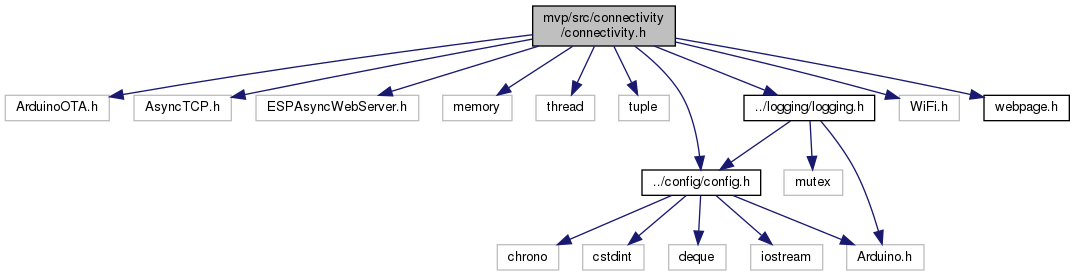
\includegraphics[width=350pt]{connectivity_8h__incl}
\end{center}
\end{figure}
This graph shows which files directly or indirectly include this file\+:
\nopagebreak
\begin{figure}[H]
\begin{center}
\leavevmode
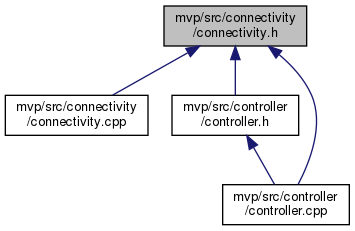
\includegraphics[width=338pt]{connectivity_8h__dep__incl}
\end{center}
\end{figure}
\subsection*{Classes}
\begin{DoxyCompactItemize}
\item 
class \hyperlink{classConnectivity}{Connectivity}
\end{DoxyCompactItemize}


\subsection{Detailed Description}
Define overall structure for class containing Wi\+Fi, O\+TA and webpage functionality. 

\begin{DoxyAuthor}{Author}
Mahimana Bhatt (\href{mailto:mahimanabhatt@gmail.com}{\tt mahimanabhatt@gmail.\+com}) 
\end{DoxyAuthor}
\begin{DoxyVersion}{Version}
0.\+1 
\end{DoxyVersion}
\begin{DoxyDate}{Date}
2022-\/07-\/19
\end{DoxyDate}
\begin{DoxyCopyright}{Copyright}
Copyright (c) 2022 
\end{DoxyCopyright}

\hypertarget{controller_8cpp}{}\section{mvp/src/controller/controller.cpp File Reference}
\label{controller_8cpp}\index{mvp/src/controller/controller.\+cpp@{mvp/src/controller/controller.\+cpp}}


Contains algorithms which controls the whole device from initialization to giving commands to every subsystem.  


{\ttfamily \#include \char`\"{}controller.\+h\char`\"{}}\newline
{\ttfamily \#include $<$Arduino.\+h$>$}\newline
{\ttfamily \#include $<$stdio.\+h$>$}\newline
{\ttfamily \#include $<$stdlib.\+h$>$}\newline
{\ttfamily \#include $<$chrono$>$}\newline
{\ttfamily \#include $<$memory$>$}\newline
{\ttfamily \#include \char`\"{}../alexa\+\_\+interaction/alexa\+\_\+interaction.\+h\char`\"{}}\newline
{\ttfamily \#include \char`\"{}../config/config.\+h\char`\"{}}\newline
{\ttfamily \#include \char`\"{}../connectivity/connectivity.\+h\char`\"{}}\newline
{\ttfamily \#include \char`\"{}../indicator/indicator.\+h\char`\"{}}\newline
{\ttfamily \#include \char`\"{}../logging/logging.\+h\char`\"{}}\newline
{\ttfamily \#include \char`\"{}../manual\+\_\+interaction/manual\+\_\+interaction.\+h\char`\"{}}\newline
{\ttfamily \#include \char`\"{}../motor\+\_\+driver/motor\+\_\+driver.\+h\char`\"{}}\newline
{\ttfamily \#include \char`\"{}../storage/storage.\+h\char`\"{}}\newline
Include dependency graph for controller.\+cpp\+:
\nopagebreak
\begin{figure}[H]
\begin{center}
\leavevmode
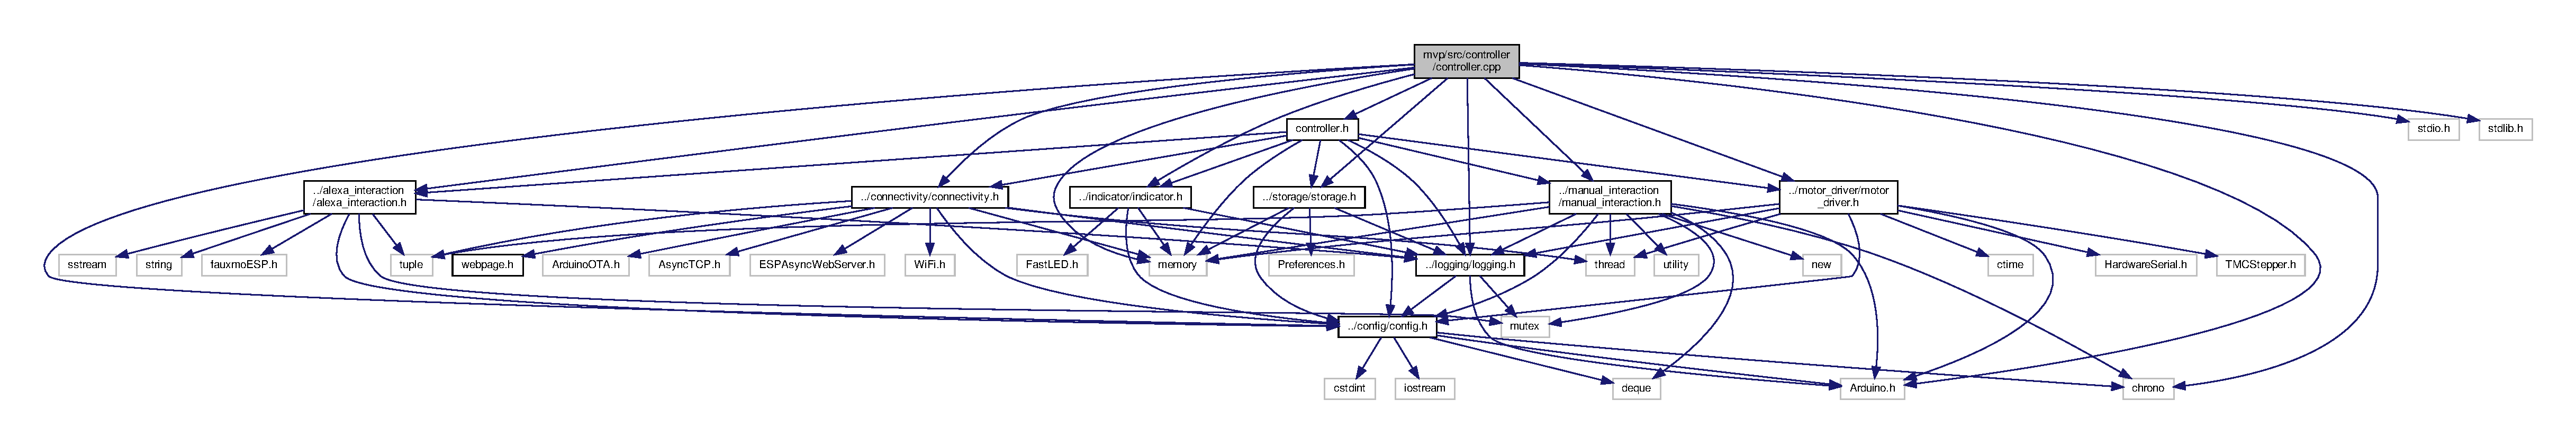
\includegraphics[width=350pt]{controller_8cpp__incl}
\end{center}
\end{figure}


\subsection{Detailed Description}
Contains algorithms which controls the whole device from initialization to giving commands to every subsystem. 

\begin{DoxyAuthor}{Author}
Dhiraj Deshmukh (\href{mailto:deshmukhdhiraj15@gmail.com}{\tt deshmukhdhiraj15@gmail.\+com}) 
\end{DoxyAuthor}
\begin{DoxyVersion}{Version}
0.\+1 
\end{DoxyVersion}
\begin{DoxyDate}{Date}
2022-\/07-\/19
\end{DoxyDate}
\begin{DoxyCopyright}{Copyright}
Copyright (c) 2022 
\end{DoxyCopyright}

\hypertarget{controller_8h}{}\section{mvp/src/controller/controller.h File Reference}
\label{controller_8h}\index{mvp/src/controller/controller.\+h@{mvp/src/controller/controller.\+h}}


Defines the structure of the main controller of the device.  


{\ttfamily \#include $<$memory$>$}\newline
{\ttfamily \#include \char`\"{}../alexa\+\_\+interaction/alexa\+\_\+interaction.\+h\char`\"{}}\newline
{\ttfamily \#include \char`\"{}../config/config.\+h\char`\"{}}\newline
{\ttfamily \#include \char`\"{}../connectivity/connectivity.\+h\char`\"{}}\newline
{\ttfamily \#include \char`\"{}../indicator/indicator.\+h\char`\"{}}\newline
{\ttfamily \#include \char`\"{}../logging/logging.\+h\char`\"{}}\newline
{\ttfamily \#include \char`\"{}../manual\+\_\+interaction/manual\+\_\+interaction.\+h\char`\"{}}\newline
{\ttfamily \#include \char`\"{}../motor\+\_\+driver/motor\+\_\+driver.\+h\char`\"{}}\newline
{\ttfamily \#include \char`\"{}../storage/storage.\+h\char`\"{}}\newline
Include dependency graph for controller.\+h\+:
\nopagebreak
\begin{figure}[H]
\begin{center}
\leavevmode
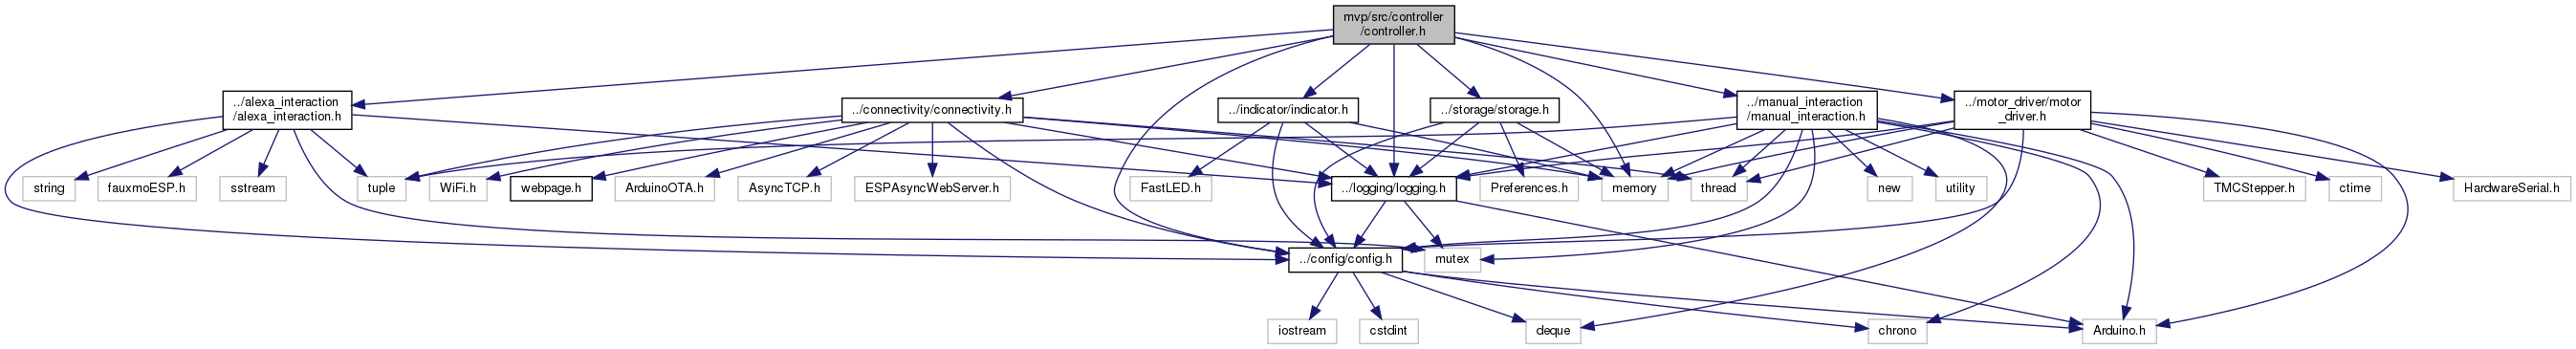
\includegraphics[width=350pt]{controller_8h__incl}
\end{center}
\end{figure}
This graph shows which files directly or indirectly include this file\+:
\nopagebreak
\begin{figure}[H]
\begin{center}
\leavevmode
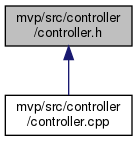
\includegraphics[width=175pt]{controller_8h__dep__incl}
\end{center}
\end{figure}
\subsection*{Classes}
\begin{DoxyCompactItemize}
\item 
class \hyperlink{classController}{Controller}
\end{DoxyCompactItemize}


\subsection{Detailed Description}
Defines the structure of the main controller of the device. 

\begin{DoxyAuthor}{Author}
Mahimana Bhatt (\href{mailto:mahimanabhatt@gmail.com}{\tt mahimanabhatt@gmail.\+com}) 
\end{DoxyAuthor}
\begin{DoxyVersion}{Version}
0.\+1 
\end{DoxyVersion}
\begin{DoxyDate}{Date}
2022-\/07-\/19
\end{DoxyDate}
\begin{DoxyCopyright}{Copyright}
Copyright (c) 2022 
\end{DoxyCopyright}

\hypertarget{indicator_8cpp}{}\section{mvp/src/indicator/indicator.cpp File Reference}
\label{indicator_8cpp}\index{mvp/src/indicator/indicator.\+cpp@{mvp/src/indicator/indicator.\+cpp}}


Contains algorithms for R\+GB L\+ED.  


{\ttfamily \#include \char`\"{}indicator.\+h\char`\"{}}\newline
{\ttfamily \#include $<$Fast\+L\+E\+D.\+h$>$}\newline
{\ttfamily \#include \char`\"{}../config/config.\+h\char`\"{}}\newline
{\ttfamily \#include \char`\"{}../logging/logging.\+h\char`\"{}}\newline
Include dependency graph for indicator.\+cpp\+:
\nopagebreak
\begin{figure}[H]
\begin{center}
\leavevmode
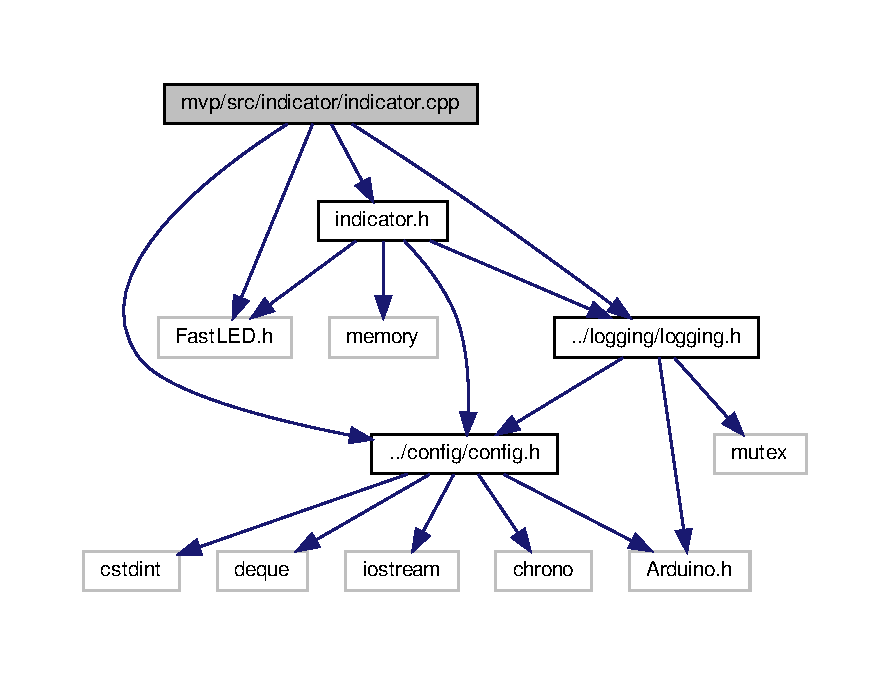
\includegraphics[width=350pt]{indicator_8cpp__incl}
\end{center}
\end{figure}


\subsection{Detailed Description}
Contains algorithms for R\+GB L\+ED. 

\begin{DoxyAuthor}{Author}
Dhiraj Deshmukh (\href{mailto:deshmukhdhiraj15@gmail.com}{\tt deshmukhdhiraj15@gmail.\+com}) 
\end{DoxyAuthor}
\begin{DoxyVersion}{Version}
0.\+1 
\end{DoxyVersion}
\begin{DoxyDate}{Date}
2022-\/07-\/19
\end{DoxyDate}
\begin{DoxyCopyright}{Copyright}
Copyright (c) 2022 
\end{DoxyCopyright}

\hypertarget{indicator_8h}{}\section{/home/mahi/git/automatic\+\_\+curtain/mvp/src/indicator/indicator.h File Reference}
\label{indicator_8h}\index{/home/mahi/git/automatic\+\_\+curtain/mvp/src/indicator/indicator.\+h@{/home/mahi/git/automatic\+\_\+curtain/mvp/src/indicator/indicator.\+h}}


Contains structure for R\+GB L\+ED (C\+OM 11821), uses F\+A\+S\+T\+Led library for controlling the L\+ED.  


\subsection*{Classes}
\begin{DoxyCompactItemize}
\item 
class \hyperlink{classIndicator}{Indicator}
\end{DoxyCompactItemize}


\subsection{Detailed Description}
Contains structure for R\+GB L\+ED (C\+OM 11821), uses F\+A\+S\+T\+Led library for controlling the L\+ED. 

\begin{DoxyAuthor}{Author}
Mahimana Bhatt (\href{mailto:mahimanabhatt@gmail.com}{\tt mahimanabhatt@gmail.\+com}) 
\end{DoxyAuthor}
\begin{DoxyVersion}{Version}
0.\+1 
\end{DoxyVersion}
\begin{DoxyDate}{Date}
2022-\/07-\/19
\end{DoxyDate}
\begin{DoxyCopyright}{Copyright}
Copyright (c) 2022 
\end{DoxyCopyright}

\hypertarget{logging_8cpp}{}\section{mvp/src/logging/logging.cpp File Reference}
\label{logging_8cpp}\index{mvp/src/logging/logging.\+cpp@{mvp/src/logging/logging.\+cpp}}


Contains all algorithms for maintaing device logs.  


{\ttfamily \#include \char`\"{}logging.\+h\char`\"{}}\newline
{\ttfamily \#include $<$Arduino.\+h$>$}\newline
{\ttfamily \#include $<$mutex$>$}\newline
{\ttfamily \#include \char`\"{}../config/config.\+h\char`\"{}}\newline
Include dependency graph for logging.\+cpp\+:
\nopagebreak
\begin{figure}[H]
\begin{center}
\leavevmode
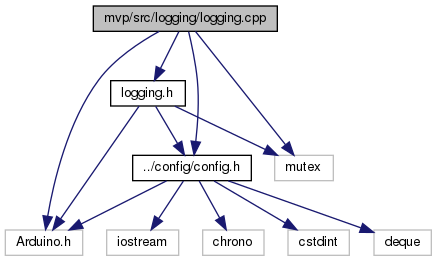
\includegraphics[width=350pt]{logging_8cpp__incl}
\end{center}
\end{figure}


\subsection{Detailed Description}
Contains all algorithms for maintaing device logs. 

\begin{DoxyAuthor}{Author}
Dhiraj Deshmukh (\href{mailto:deshmukhdhiraj15@gmail.com}{\tt deshmukhdhiraj15@gmail.\+com}) 
\end{DoxyAuthor}
\begin{DoxyVersion}{Version}
0.\+1 
\end{DoxyVersion}
\begin{DoxyDate}{Date}
2022-\/07-\/19
\end{DoxyDate}
\begin{DoxyCopyright}{Copyright}
Copyright (c) 2022 
\end{DoxyCopyright}

\hypertarget{logging_8h}{}\section{mvp/src/logging/logging.h File Reference}
\label{logging_8h}\index{mvp/src/logging/logging.\+h@{mvp/src/logging/logging.\+h}}


Defines code structure for logging of device.  


{\ttfamily \#include $<$Arduino.\+h$>$}\newline
{\ttfamily \#include $<$mutex$>$}\newline
{\ttfamily \#include \char`\"{}../config/config.\+h\char`\"{}}\newline
Include dependency graph for logging.\+h\+:
\nopagebreak
\begin{figure}[H]
\begin{center}
\leavevmode
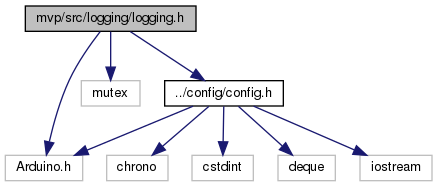
\includegraphics[width=350pt]{logging_8h__incl}
\end{center}
\end{figure}
This graph shows which files directly or indirectly include this file\+:
\nopagebreak
\begin{figure}[H]
\begin{center}
\leavevmode
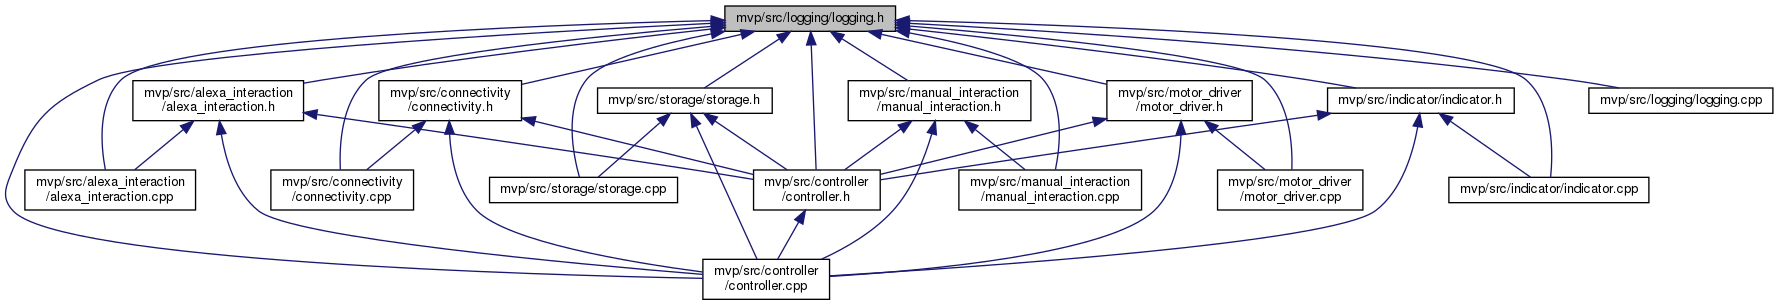
\includegraphics[width=350pt]{logging_8h__dep__incl}
\end{center}
\end{figure}
\subsection*{Classes}
\begin{DoxyCompactItemize}
\item 
class \hyperlink{classLogging}{Logging}
\end{DoxyCompactItemize}


\subsection{Detailed Description}
Defines code structure for logging of device. 

\begin{DoxyAuthor}{Author}
Mahimana Bhatt (\href{mailto:mahimanabhatt@gmail.com}{\tt mahimanabhatt@gmail.\+com}) 
\end{DoxyAuthor}
\begin{DoxyVersion}{Version}
0.\+1 
\end{DoxyVersion}
\begin{DoxyDate}{Date}
2022-\/07-\/19
\end{DoxyDate}
\begin{DoxyCopyright}{Copyright}
Copyright (c) 2022 
\end{DoxyCopyright}

\hypertarget{manual__interaction_8cpp}{}\section{mvp/src/manual\+\_\+interaction/manual\+\_\+interaction.cpp File Reference}
\label{manual__interaction_8cpp}\index{mvp/src/manual\+\_\+interaction/manual\+\_\+interaction.\+cpp@{mvp/src/manual\+\_\+interaction/manual\+\_\+interaction.\+cpp}}


Contains algorithms to detect a users manual interaction with the device, specifically push buttons.  


{\ttfamily \#include \char`\"{}manual\+\_\+interaction.\+h\char`\"{}}\newline
{\ttfamily \#include $<$Arduino.\+h$>$}\newline
{\ttfamily \#include $<$chrono$>$}\newline
{\ttfamily \#include $<$deque$>$}\newline
{\ttfamily \#include $<$memory$>$}\newline
{\ttfamily \#include $<$mutex$>$}\newline
{\ttfamily \#include $<$new$>$}\newline
{\ttfamily \#include $<$tuple$>$}\newline
{\ttfamily \#include $<$utility$>$}\newline
{\ttfamily \#include \char`\"{}../config/config.\+h\char`\"{}}\newline
{\ttfamily \#include \char`\"{}../logging/logging.\+h\char`\"{}}\newline
Include dependency graph for manual\+\_\+interaction.\+cpp\+:
\nopagebreak
\begin{figure}[H]
\begin{center}
\leavevmode
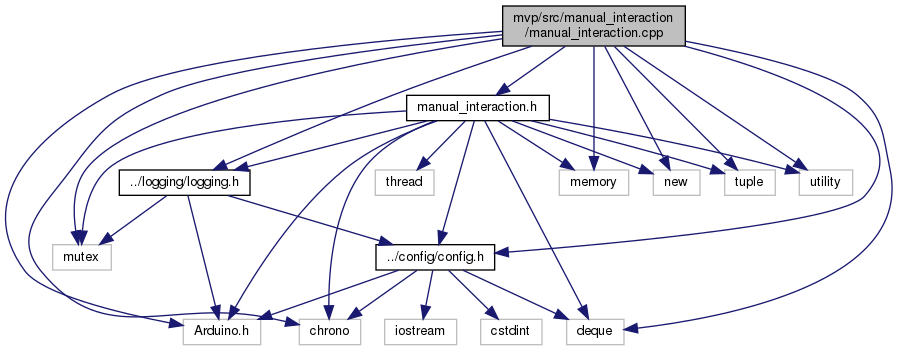
\includegraphics[width=350pt]{manual__interaction_8cpp__incl}
\end{center}
\end{figure}


\subsection{Detailed Description}
Contains algorithms to detect a users manual interaction with the device, specifically push buttons. 

\begin{DoxyAuthor}{Author}
Dhiraj Deshmukh (\href{mailto:deshmukhdhiraj15@gmail.com}{\tt deshmukhdhiraj15@gmail.\+com}) 
\end{DoxyAuthor}
\begin{DoxyVersion}{Version}
0.\+1 
\end{DoxyVersion}
\begin{DoxyDate}{Date}
2022-\/07-\/19
\end{DoxyDate}
\begin{DoxyCopyright}{Copyright}
Copyright (c) 2022 
\end{DoxyCopyright}

\hypertarget{manual__interaction_8h}{}\section{mvp/src/manual\+\_\+interaction/manual\+\_\+interaction.h File Reference}
\label{manual__interaction_8h}\index{mvp/src/manual\+\_\+interaction/manual\+\_\+interaction.\+h@{mvp/src/manual\+\_\+interaction/manual\+\_\+interaction.\+h}}


Defines structure for manual interaction with device.  


{\ttfamily \#include $<$Arduino.\+h$>$}\newline
{\ttfamily \#include $<$chrono$>$}\newline
{\ttfamily \#include $<$deque$>$}\newline
{\ttfamily \#include $<$memory$>$}\newline
{\ttfamily \#include $<$mutex$>$}\newline
{\ttfamily \#include $<$new$>$}\newline
{\ttfamily \#include $<$thread$>$}\newline
{\ttfamily \#include $<$tuple$>$}\newline
{\ttfamily \#include $<$utility$>$}\newline
{\ttfamily \#include \char`\"{}../config/config.\+h\char`\"{}}\newline
{\ttfamily \#include \char`\"{}../logging/logging.\+h\char`\"{}}\newline
Include dependency graph for manual\+\_\+interaction.\+h\+:
\nopagebreak
\begin{figure}[H]
\begin{center}
\leavevmode
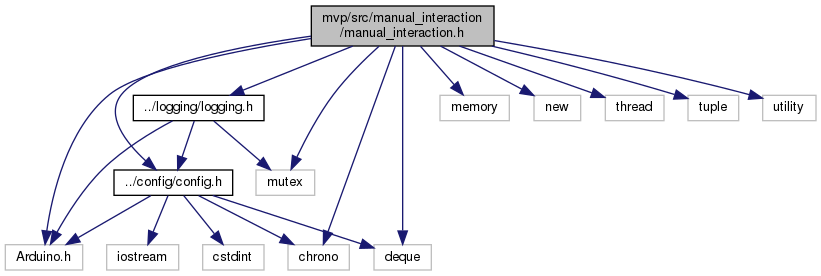
\includegraphics[width=350pt]{manual__interaction_8h__incl}
\end{center}
\end{figure}
This graph shows which files directly or indirectly include this file\+:
\nopagebreak
\begin{figure}[H]
\begin{center}
\leavevmode
\includegraphics[width=350pt]{manual__interaction_8h__dep__incl}
\end{center}
\end{figure}
\subsection*{Classes}
\begin{DoxyCompactItemize}
\item 
class \hyperlink{classManualInteraction}{Manual\+Interaction}
\end{DoxyCompactItemize}


\subsection{Detailed Description}
Defines structure for manual interaction with device. 

\begin{DoxyAuthor}{Author}
Mahimana Bhatt (\href{mailto:mahimanabhatt@gmail.com}{\tt mahimanabhatt@gmail.\+com}) 
\end{DoxyAuthor}
\begin{DoxyVersion}{Version}
0.\+1 
\end{DoxyVersion}
\begin{DoxyDate}{Date}
2022-\/07-\/19
\end{DoxyDate}
\begin{DoxyCopyright}{Copyright}
Copyright (c) 2022 
\end{DoxyCopyright}

\hypertarget{motor__driver_8cpp}{}\section{mvp/src/motor\+\_\+driver/motor\+\_\+driver.cpp File Reference}
\label{motor__driver_8cpp}\index{mvp/src/motor\+\_\+driver/motor\+\_\+driver.\+cpp@{mvp/src/motor\+\_\+driver/motor\+\_\+driver.\+cpp}}


Contains algorithms for controlling stepper motor.  


{\ttfamily \#include \char`\"{}motor\+\_\+driver.\+h\char`\"{}}\newline
{\ttfamily \#include $<$Arduino.\+h$>$}\newline
{\ttfamily \#include $<$Hardware\+Serial.\+h$>$}\newline
{\ttfamily \#include $<$T\+M\+C\+Stepper.\+h$>$}\newline
{\ttfamily \#include $<$ctime$>$}\newline
{\ttfamily \#include \char`\"{}../config/config.\+h\char`\"{}}\newline
{\ttfamily \#include \char`\"{}../logging/logging.\+h\char`\"{}}\newline
Include dependency graph for motor\+\_\+driver.\+cpp\+:
\nopagebreak
\begin{figure}[H]
\begin{center}
\leavevmode
\includegraphics[width=350pt]{motor__driver_8cpp__incl}
\end{center}
\end{figure}


\subsection{Detailed Description}
Contains algorithms for controlling stepper motor. 

\begin{DoxyAuthor}{Author}
Dhiraj Deshmukh (\href{mailto:deshmukhdhiraj15@gmail.com}{\tt deshmukhdhiraj15@gmail.\+com}) 
\end{DoxyAuthor}
\begin{DoxyVersion}{Version}
0.\+1 
\end{DoxyVersion}
\begin{DoxyDate}{Date}
2022-\/07-\/19
\end{DoxyDate}
\begin{DoxyCopyright}{Copyright}
Copyright (c) 2022 
\end{DoxyCopyright}

\hypertarget{motor__driver_8h}{}\section{/home/mahi/git/automatic\+\_\+curtain/mvp/src/motor\+\_\+driver/motor\+\_\+driver.h File Reference}
\label{motor__driver_8h}\index{/home/mahi/git/automatic\+\_\+curtain/mvp/src/motor\+\_\+driver/motor\+\_\+driver.\+h@{/home/mahi/git/automatic\+\_\+curtain/mvp/src/motor\+\_\+driver/motor\+\_\+driver.\+h}}


Defines structure for controller of stepper motor, uses library T\+M\+C2209 for this usecase.  


\subsection*{Classes}
\begin{DoxyCompactItemize}
\item 
class \hyperlink{classMotorDriver}{Motor\+Driver}
\end{DoxyCompactItemize}


\subsection{Detailed Description}
Defines structure for controller of stepper motor, uses library T\+M\+C2209 for this usecase. 

\begin{DoxyAuthor}{Author}
Mahimana Bhatt (\href{mailto:mahimanabhatt@gmail.com}{\tt mahimanabhatt@gmail.\+com}) 
\end{DoxyAuthor}
\begin{DoxyVersion}{Version}
0.\+1 
\end{DoxyVersion}
\begin{DoxyDate}{Date}
2022-\/07-\/19
\end{DoxyDate}
\begin{DoxyCopyright}{Copyright}
Copyright (c) 2022 
\end{DoxyCopyright}

\hypertarget{storage_8cpp}{}\section{/home/mahi/git/automatic\+\_\+curtain/mvp/src/storage/storage.cpp File Reference}
\label{storage_8cpp}\index{/home/mahi/git/automatic\+\_\+curtain/mvp/src/storage/storage.\+cpp@{/home/mahi/git/automatic\+\_\+curtain/mvp/src/storage/storage.\+cpp}}


Contains algorithms to read and write appropriate device data to E\+E\+P\+R\+OM.  




\subsection{Detailed Description}
Contains algorithms to read and write appropriate device data to E\+E\+P\+R\+OM. 

\begin{DoxyAuthor}{Author}
Dhiraj Deshmukh (\href{mailto:deshmukhdhiraj15@gmail.com}{\tt deshmukhdhiraj15@gmail.\+com}) 
\end{DoxyAuthor}
\begin{DoxyVersion}{Version}
0.\+1 
\end{DoxyVersion}
\begin{DoxyDate}{Date}
2022-\/07-\/19
\end{DoxyDate}
\begin{DoxyCopyright}{Copyright}
Copyright (c) 2022 
\end{DoxyCopyright}

\hypertarget{storage_8h}{}\section{mvp/src/storage/storage.h File Reference}
\label{storage_8h}\index{mvp/src/storage/storage.\+h@{mvp/src/storage/storage.\+h}}


Defines structure for Flash storage for E\+S\+P32.  


{\ttfamily \#include $<$Preferences.\+h$>$}\newline
{\ttfamily \#include $<$memory$>$}\newline
{\ttfamily \#include \char`\"{}../config/config.\+h\char`\"{}}\newline
{\ttfamily \#include \char`\"{}../logging/logging.\+h\char`\"{}}\newline
Include dependency graph for storage.\+h\+:
\nopagebreak
\begin{figure}[H]
\begin{center}
\leavevmode
\includegraphics[width=350pt]{storage_8h__incl}
\end{center}
\end{figure}
This graph shows which files directly or indirectly include this file\+:
\nopagebreak
\begin{figure}[H]
\begin{center}
\leavevmode
\includegraphics[width=350pt]{storage_8h__dep__incl}
\end{center}
\end{figure}
\subsection*{Classes}
\begin{DoxyCompactItemize}
\item 
class \hyperlink{classStorage}{Storage}
\end{DoxyCompactItemize}


\subsection{Detailed Description}
Defines structure for Flash storage for E\+S\+P32. 

\begin{DoxyAuthor}{Author}
Mahimana Bhatt (\href{mailto:mahimanabhatt@gmail.com}{\tt mahimanabhatt@gmail.\+com}) 
\end{DoxyAuthor}
\begin{DoxyVersion}{Version}
0.\+1 
\end{DoxyVersion}
\begin{DoxyDate}{Date}
2022-\/07-\/19
\end{DoxyDate}
\begin{DoxyCopyright}{Copyright}
Copyright (c) 2022 
\end{DoxyCopyright}

%--- End generated contents ---

% Index
\backmatter
\newpage
\phantomsection
\clearemptydoublepage
\addcontentsline{toc}{chapter}{Index}
\printindex

\end{document}
